\documentclass[a4paper,reqno,]{article}
\usepackage[utf8]{inputenc}
\usepackage[english]{babel}
\usepackage[nosumlimits]{amsmath}
\usepackage{graphicx}
\usepackage{fancyhdr}
\usepackage{hyperref}
%\usepackage{adjustbox}
%\usepackage{array}
\usepackage{array,booktabs,enumitem}
\usepackage{caption}
\usepackage{bm}
\usepackage{todonotes}
\usepackage{ctable}
\usepackage[acronym]{glossaries}
\usepackage{subcaption}
\usepackage[left=2cm,right=2cm,top=2.5cm,includeheadfoot]{geometry}
\usepackage{listings}
\usepackage{color, colortbl}
\usepackage{longtable}
\definecolor{Gray}{gray}{0.8}
\newlength{\Oldarrayrulewidth}
\usepackage{booktabs}
\newcommand{\Cline}[2]{%
  \noalign{\global\setlength{\Oldarrayrulewidth}{\arrayrulewidth}}%
  \noalign{\global\setlength{\arrayrulewidth}{#1}}\cline{#2}%
  \noalign{\global\setlength{\arrayrulewidth}{\Oldarrayrulewidth}}}
\renewcommand\lstlistingname{Beispiel}
\usepackage[export]{adjustbox}
\newcommand{\dd}[1]{\mathrm{d}#1}
\usepackage{float}
%\usepackage[backend=biber,style=apa, citestyle=authoryear, sorting=nty]{biblatex}
\usepackage[backend=biber,style=authoryear, sorting=nty]{biblatex}
\setlength{\bibitemsep}{\baselineskip}
%\DeclareLanguageMapping{american}{american-apa}
%\usepackage[super]{biber}
%\makeatletter 
%\renewcommand\@biblabel[1]{} 
%\makeatother
\addbibresource{references.bib}
\begin{document}
\begin{titlepage}
\centering
{\scshape University College London \par}
{\scshape Faculty of Engineering Sciences \par}
\vspace{1cm}
\begin{minipage}[b]{1\textwidth}
\centering
    
\includegraphics[width=0.3\textwidth]{images/ucl_logo.jpg}
\end{minipage}
\newline
\newline
\newline
{\large\bfseries CEGEG076 Spatio-Temporal Data Mining \par}
\vspace{1.5cm}
{\huge\bfseries  Spatio-Temporal Analysis on: \\
 Forecasting Tourist Data in Austria\par}
\vspace{3cm}
{\large Qiqing Huang, 17014982, ANN \par}
\vspace{0.25cm}
{\large Supratim Banik, 16118558, SVM \par}
\vspace{0.25cm}
{\large Florian Hübscher, 17135943, STARIMA \par}
\vspace{0.25cm}
{\large Claudio Navacchi, 18003316, RFR \par}
\vspace{3cm}
{Department of Civil, Environmental and Geomatic Engineering \par}
{4$^{\text{th}}$ May, 2018 \par}
\end{titlepage}
\tableofcontents
\newpage
\pagestyle{fancy}
\fancyhf{}
\setlength{\headheight}{25pt}
\headsep=30pt
\rfoot{\thepage}
\renewcommand{\headrulewidth}{0.4pt}
\fancyhead[L]{Forecasting Tourist Data in Austria}
\section{Introduction}
\fancyhead[R]{Introduction}
\label{sec:intro}
The aim of this report is to apply the methods and techniques presented in the lecture \textit{"Spatio-Temporal Data Mining"} on a spatio-temporal dataset. A dataset description is provided in subsection \ref{ssec:dataset_desc}. The subsequent section \ref{sec:expl_anal} provides an analysis of the dataset focusing on temporal (subsection \ref{ssec:t_pat}), spatial (subsection \ref{ssec:s_pat}) and spatio-temporal patterns (subsection \ref{ssec:st_pat}).   
\\
\\
The structure of the dataset restricts the applicability of the methods learned on spatio-temporal regression and prediction being the main focus of this work (subsection \ref{ssec:exp_setup}). The four methods chosen are: \textit{Random Forest Regression (RFR)} (subsection \ref{ssec:rfr}), \textit{Spatio-Temporal Auto-Regressive Integrated Moving Average (STARIMA)} (subsection \ref{ssec:starima}), \textit{Artificial Neural Networks (ANNs)} (subsection \ref{ssec:ann}) and  \textit{Support Vector Machine (SVM)}(subsection \ref{ssec:svm}). \cite{rf_manual} offers a documentation of random forests in \textit{R} following the papers/manuals \cite{breiman2001random} and \cite{rf_usage_manual}. Use case examples of \textit{RFR} can be found in \cite{liaw2002classification} and \cite{segal2004machine}. \textit{STARIMA} is proposed and documented in \cite{pfeifer1981seasonal}. Recent applications and extensions are described in \cite{Islam-KhanRezwan2012PTTi}, \cite{ChengTao2014ADSW} and \cite{PeiboDuan2016Stpw}. Systematic introduction of ANNs can be found in \citeauthor{rojas2013neural}'s book (2013). The application of ANNs in forecasting has been well concluded by \citeauthor{zhang1998forecasting} (1998) and has been widely used in tourism area (\cite{law1999neural}, \cite{burger2001practitioners}, \cite{claveria2014forecasting}). In case of the investigation using SVM/SVR, the research paper on application of support vector regression on tourism by \cite{e} and \cite{f} provided a rich source for reference. While the tutorial on support vector machine by \cite{c} helped in understanding the SVR methodology.  
\\
\\
Finally, all methods will be compared regarding meaningful statistics used for time-series analysis and an outlook for improvements will be given (section \ref{sec:disc_and_outl}). 
\subsection{Dataset Description}
\label{ssec:dataset_desc}
Tourist data in Austria including two spatio-temporal variables, namely tourist arrivals and nights spent (stays), was chosen to be the dataset of interest \footnote{download available under https://www.data.gv.at/katalog/en/dataset/128e3b47-1e44-3791-bee2-3b06b2cd58f4}. It is available monthly-wise from 11/1973 until 11/2017. The spatial resolution is defined by the nine provinces of Austria. The variables are further subdivided by the country of origin. An exemplary depiction of the first three rows is shown in table \ref{tab:data_examp}.
\newcolumntype{g}{>{\columncolor{Gray}}l}
\begin{longtable}[h!]
{!{\vrule width0.05cm}g!{\vrule width0.05cm}g!{\vrule width0.05cm}g!{\vrule width0.05cm}g!{\vrule width0.05cm}g!{\vrule width0.05cm}}
\caption{Data excerpt of the Austrian tourist dataset (top three rows).}
\label{tab:data_examp}\\
\specialrule{0.05cm}{.0cm}{.0cm}
\multicolumn{1}{!{\vrule width0.05cm}c!{\vrule width0.05cm}}{\bfseries Date \par} & \multicolumn{1}{c!{\vrule width0.05cm}}{\bfseries Province Code \par} & \multicolumn{1}{c!{\vrule width0.05cm}}{\bfseries Country of Origin Code \par} & \multicolumn{1}{c!{\vrule width0.05cm}}{\bfseries Arrivals \par} &
\multicolumn{1}{c!{\vrule width0.05cm}}{\bfseries Stays \par} \\ 
\specialrule{0.05cm}{.0cm}{.0cm} 
197311 & W96-1 & 01 & 1792 & 14288 \\ \specialrule{0.025cm}{.0cm}{.0cm}
\rowcolor{white}197311 & W96-1 & 02 & 3845 & 18901 \\ \specialrule{0.025cm}{.0cm}{.0cm}
197311 & W96-1 & 53 & 2 & 23 \\ \specialrule{0.05cm}{.0cm}{.0cm}
\end{longtable}
\noindent
Figure \ref{fig:tourist_stays_summary} shows all tourist stays and arrivals aggregated by year. A spatial view is given by fig. \ref{fig:tourist_stays_map}. 
\subsection{Experimental Setup}
\label{ssec:exp_setup}
It has been decided to predict the stays, since it is a more valuable parameter for tourism than arrivals. Each regression model should be trained and validated from 11/1973 to 12/2010 and from 01/2011 to 11/2017, respectively. All countries of origin were aggregated province-wise over time to simplify the dataset. Additionally, prediction success should be evaluated by using statistics such as RMSE and R$^2$ and n-step ahead instead of one-step ahead prediction.
\newpage
\begin{figure}[h!]
\begin{minipage}[b]{1\textwidth}
\centering
    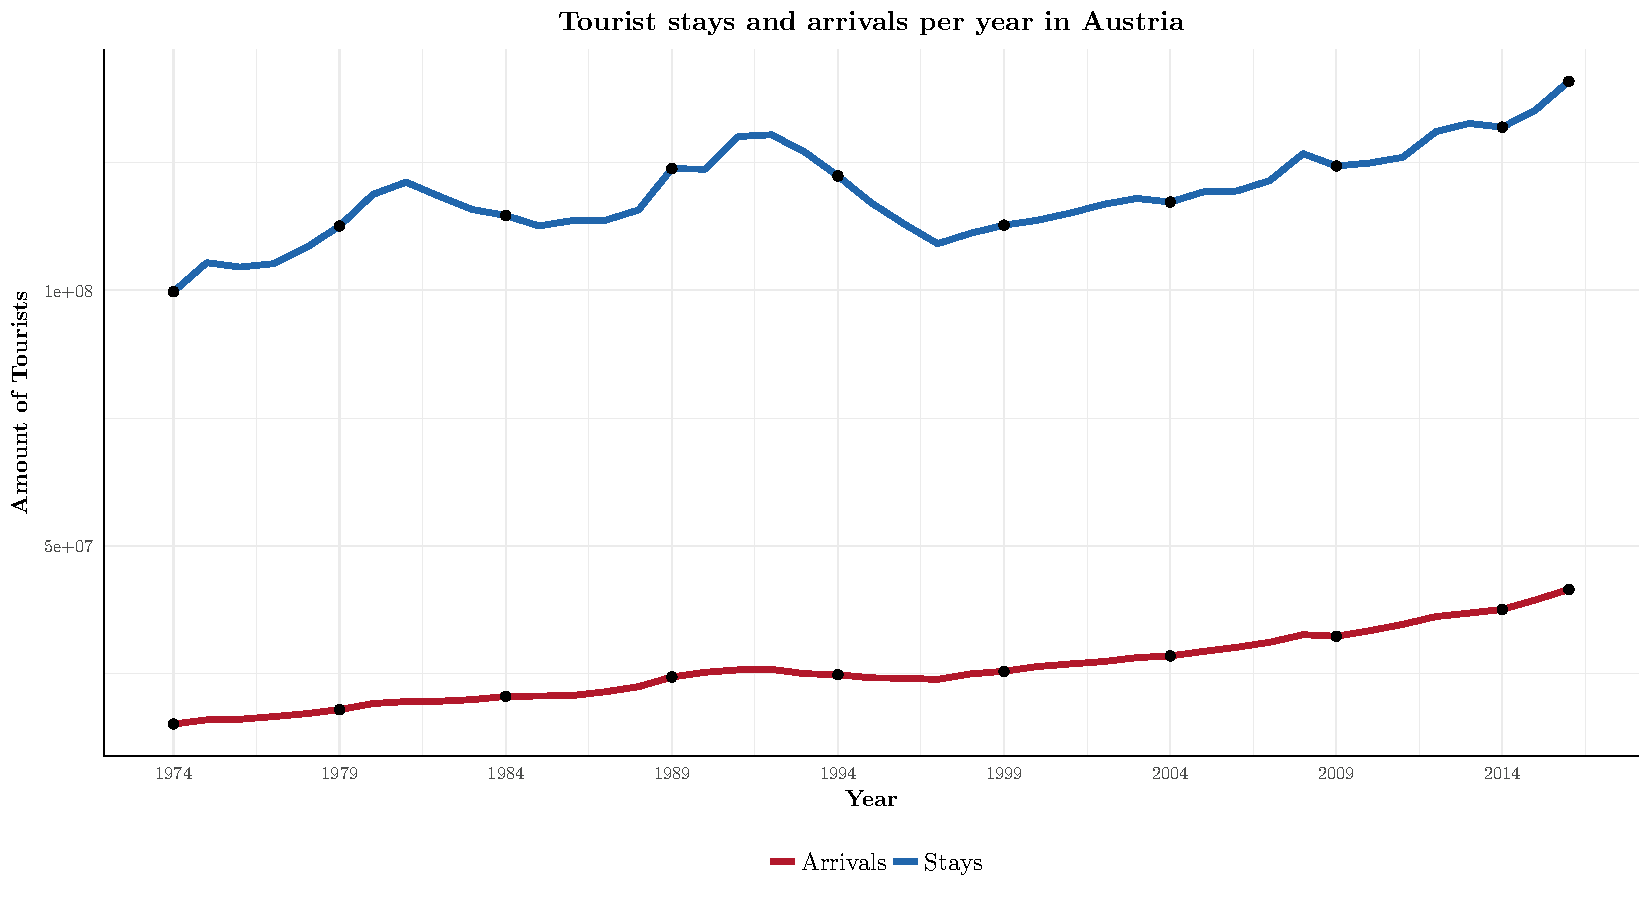
\includegraphics[width=0.8\textwidth]{images/EA/tourist_stays_summary.pdf}
    \caption{Aggregated tourist data depicting stays over night and arrivals. A clear trend is visible for both, whereas stays are characterised by larger fluctuations over time (weather conditions, advertisment, sport events, ...). A trend could be also caused by more accommodations taking part (or must take part) in the national collection of tourist data.}
\label{fig:tourist_stays_summary}
\end{minipage}
\end{figure} 
\begin{figure}[h!]
\begin{minipage}[b]{1\textwidth}
\centering
    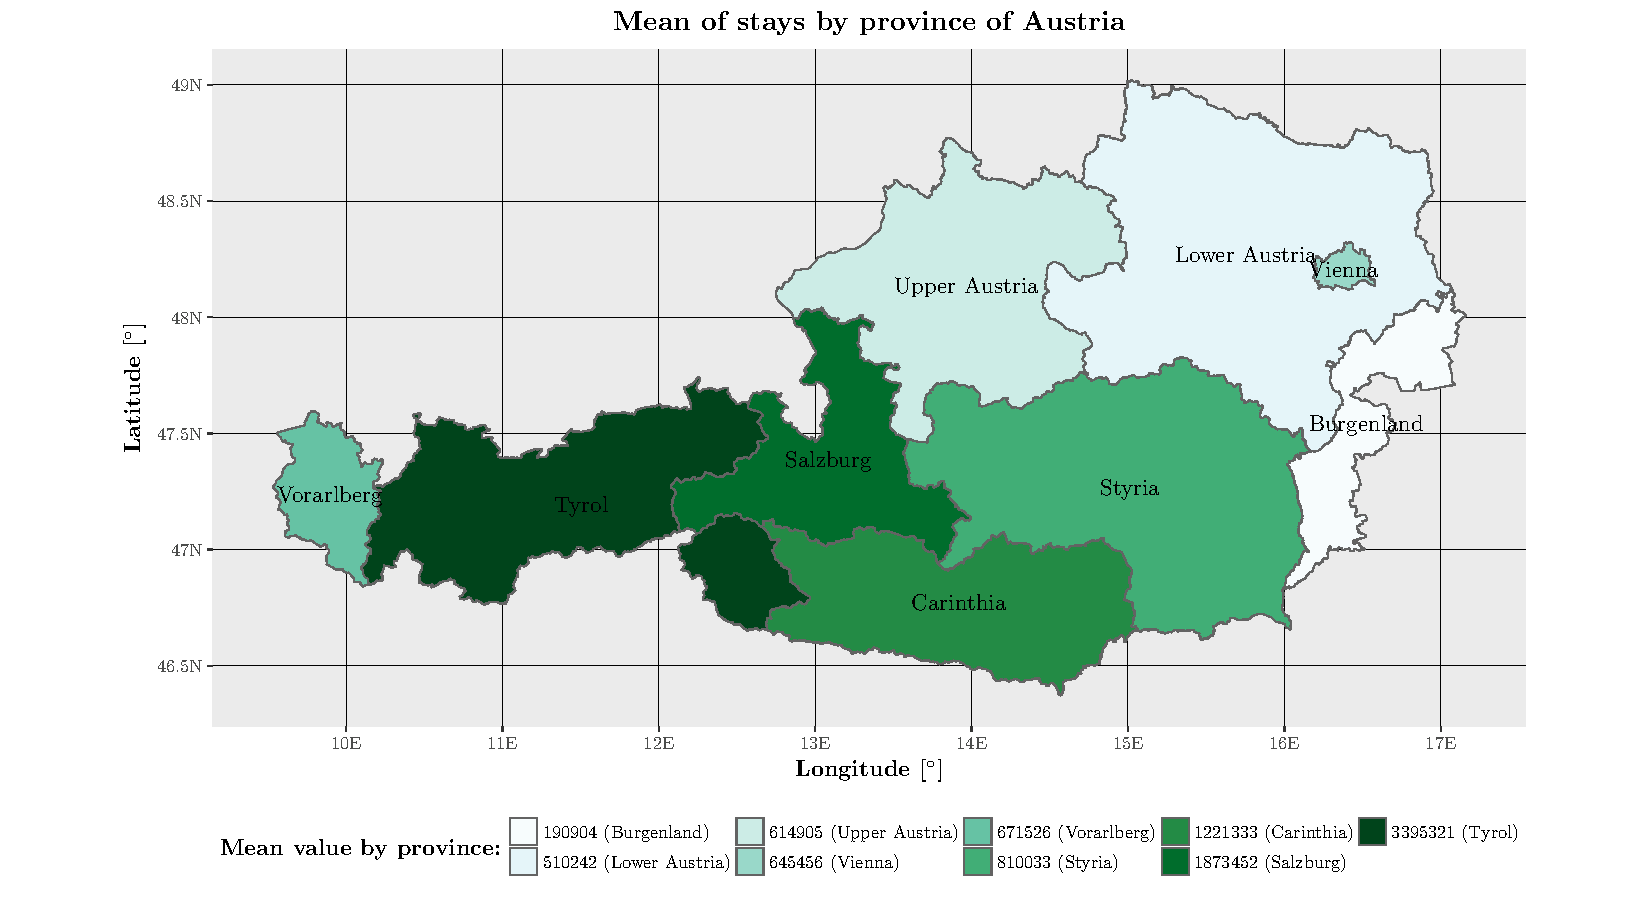
\includegraphics[width=0.8\textwidth]{images/EA/provinces_stays_mean.pdf}
    \caption{Austrian map showing the mean value of tourist stays per province from 1973-2017. The mountainous regions in the western part of Austria offer a broad spectrum of leisure activities, which is more attractive for longer stays, followed by Vienna being popular for its culture and history (short-time visits). All other provinces seem to be of minor importance for tourists.}
       \label{fig:tourist_stays_map}
\end{minipage}
\end{figure} 
\newpage
\section{Exploratory Spatio-Temporal Data Analysis}
\label{sec:expl_anal}
\fancyhead[R]{Exploratory Spatio-Temporal Data Analysis}
\subsection{Temporal Patterns}
\label{ssec:t_pat}
The heatmap in figure \ref{fig:heat} provides an overview of overnight tourist stays across Austria. It can be seen that Tyrol, Carinthia and Salzburg have the highest values and some provinces have two peaks while others have one. Carinthia is the most significant province having a descending trend.
\begin{figure}[h!]
\begin{minipage}[b]{1\textwidth}
\centering
    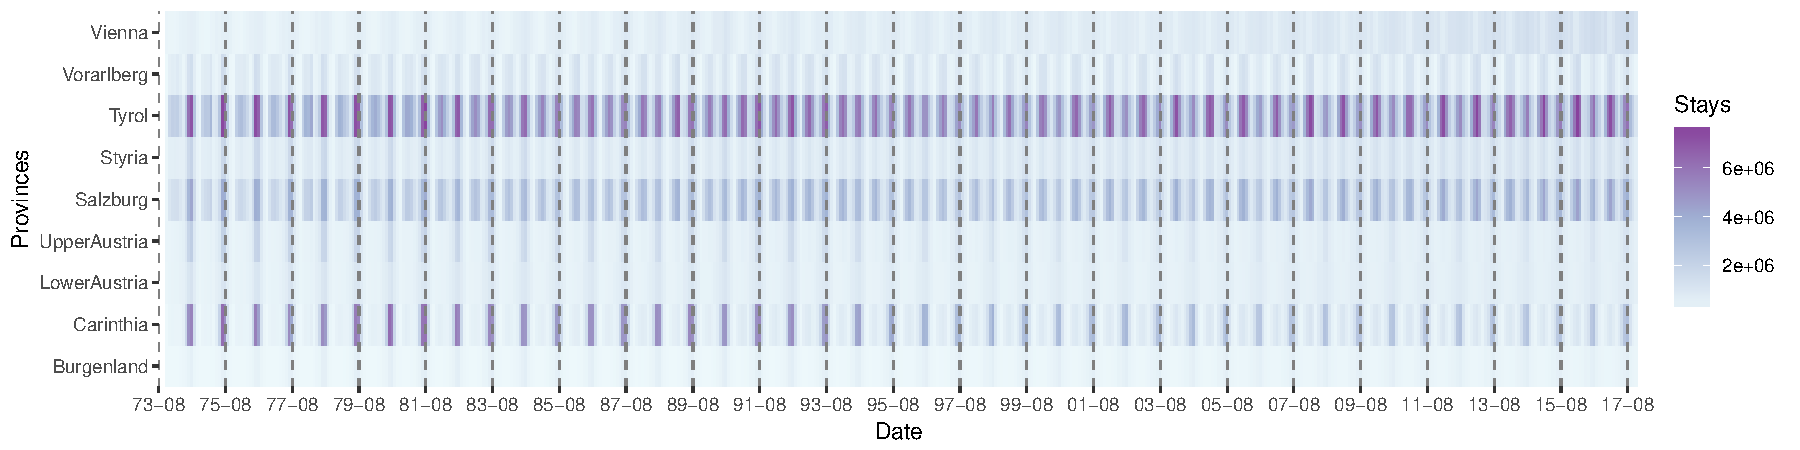
\includegraphics[width=1\textwidth]{images/EA/Heatmap.pdf}
    \caption{Heatmap of overnight stays time series.}\label{fig:heat}
\end{minipage}
\end{figure} 
\\
\noindent
The time series of overnight tourist stays is decomposed into a trend, seasonal and random part over time, which allows for a better understanding of stays behaviour for different provinces (see figure \ref{fig:de}). The basic equation of the classical additive decomposition method is as follows:
$$y_{t}=T_{t}+S_{t}+E_{t}$$
where trend data $T$ is computed using moving averages and seasonal data $S$ is based on average detrended values for certain periods. The time series of Vienna shows a strongly rising trend starting approximately in 2010.
\begin{figure}[h!]
\centering
\begin{minipage}[t]{1\textwidth}
\centering
    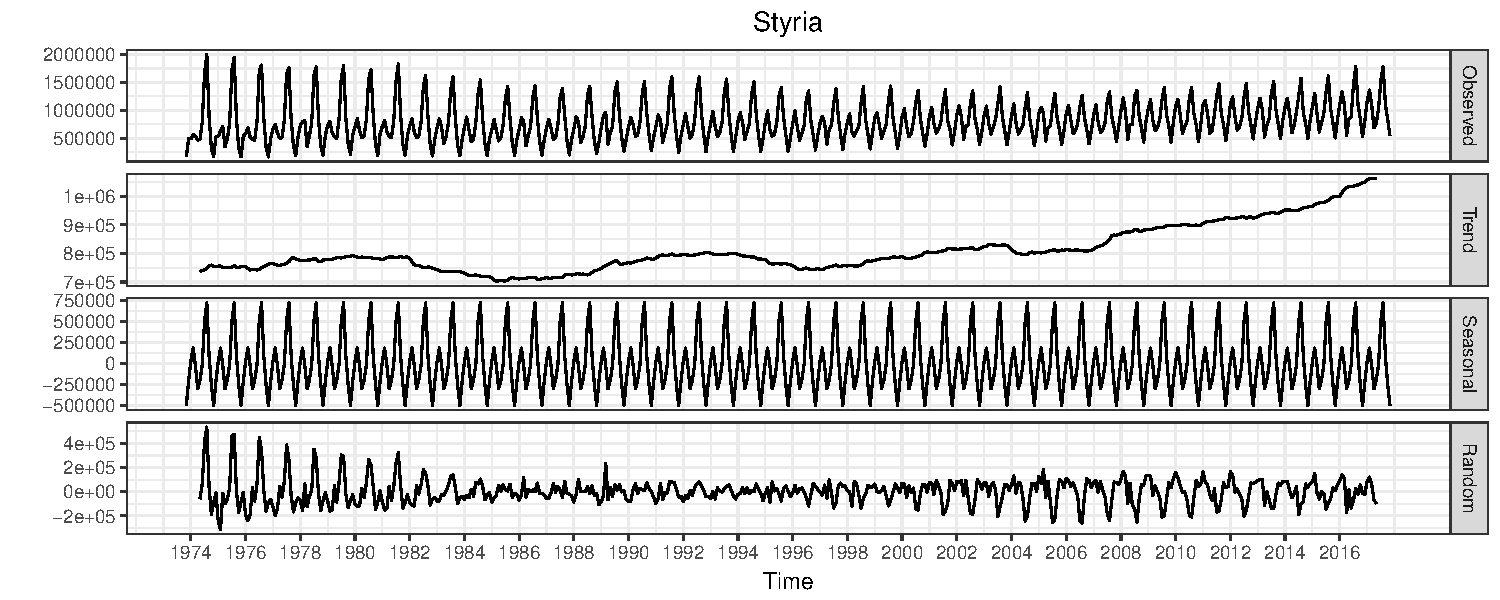
\includegraphics[width=1\textwidth]{images/EA/ts_styria.pdf}
\end{minipage}
\begin{minipage}[t]{1\textwidth}
\centering
    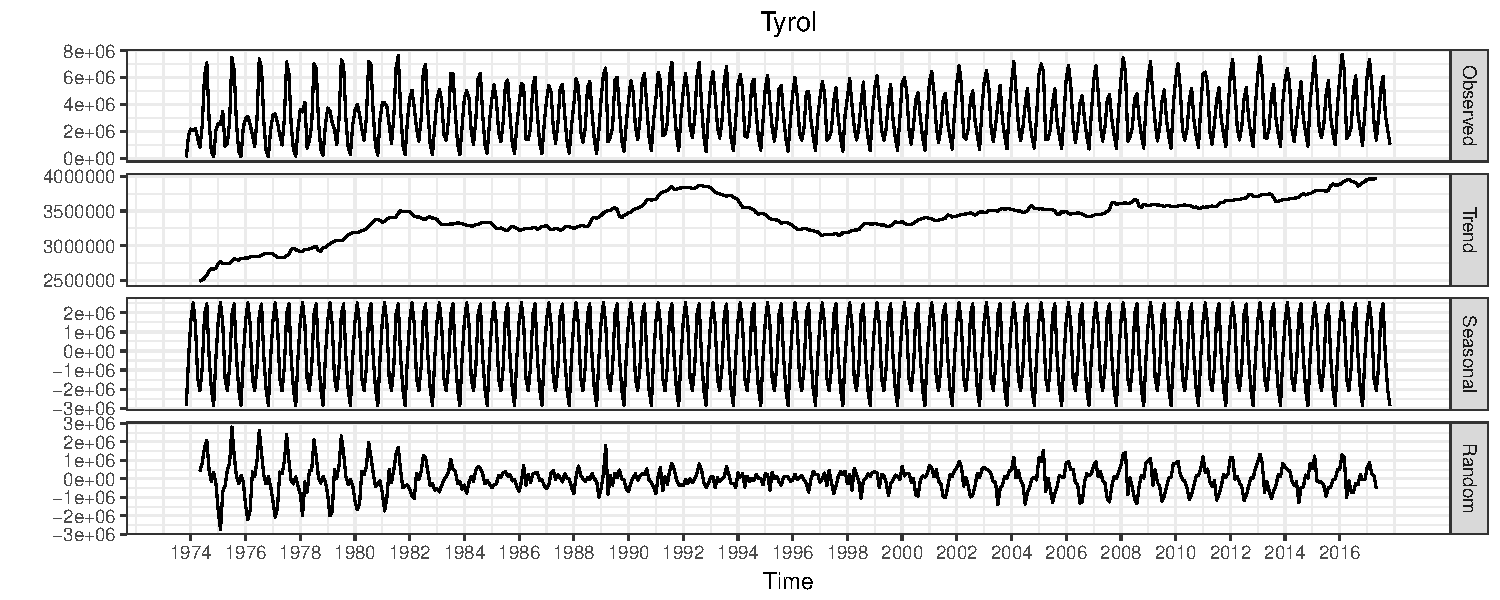
\includegraphics[width=1\textwidth]{images/EA/ts_tyrol.pdf}
\end{minipage}
\begin{minipage}[t]{1\textwidth}
\centering
    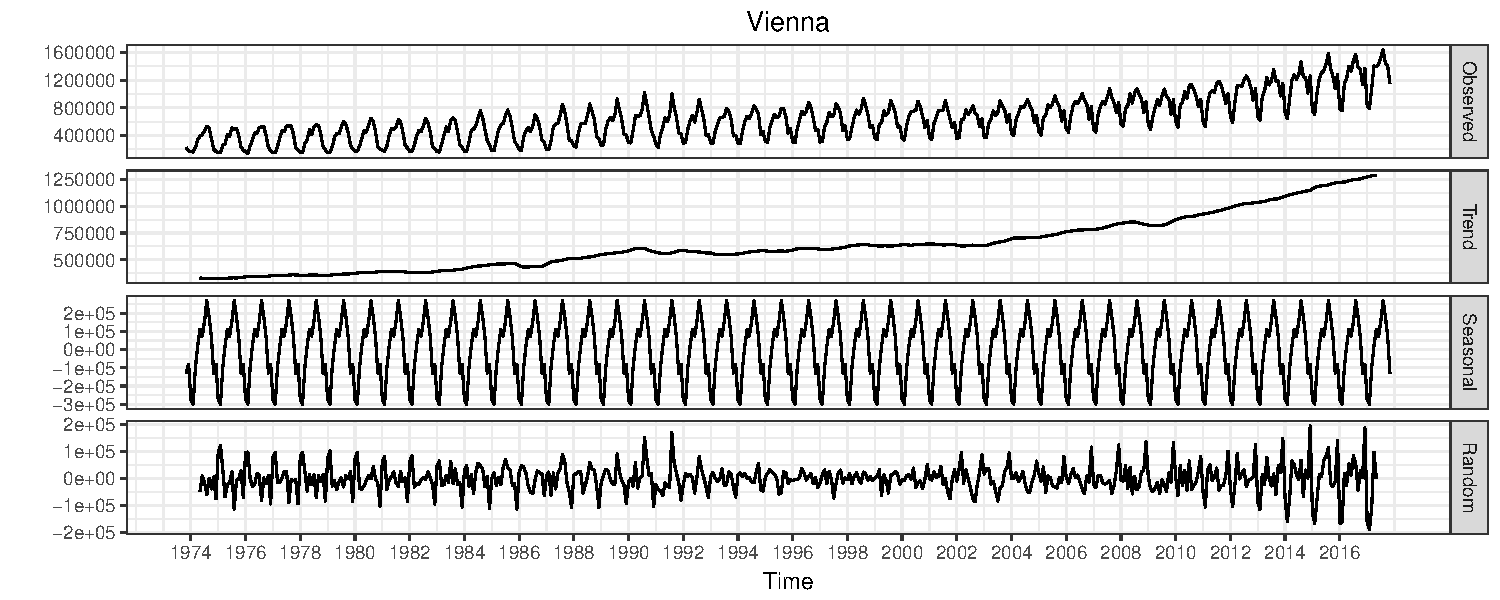
\includegraphics[width=1\textwidth]{images/EA/ts_vienna.pdf}
\end{minipage}
\caption{Decomposition of additive tourist stays time series.}\label{fig:de}
\end{figure} 
\\\\The autocorrelation function (ACF) shows for all 9 counties a predominant seasonality of order 12 (see figure \ref{fig:ACFplot}). Using monthly data this corresponds to an annual cycle. For Vienna all values are positive but slightly decaying, whereas the others alternate between negative and positive values. This suggest that the time series of Vienna is not stationary yet. Some counties show additional peaks at lag 6, 18, 30, ... which suggest that their summer and winter tourism is significant. The corresponding partial autocorrelation functions (PACF)  show consequently a large peak at lag 12 (see figure \ref{fig:PACFplot}), but usually also larger values for lag 1, 11 and 13 suggesting that the neighbouring months (and their equivalent shifted by 12 months) have an influence on the number of stays for any specific month.
\begin{figure}[h!]
\begin{minipage}[b]{1\textwidth}
\centering
    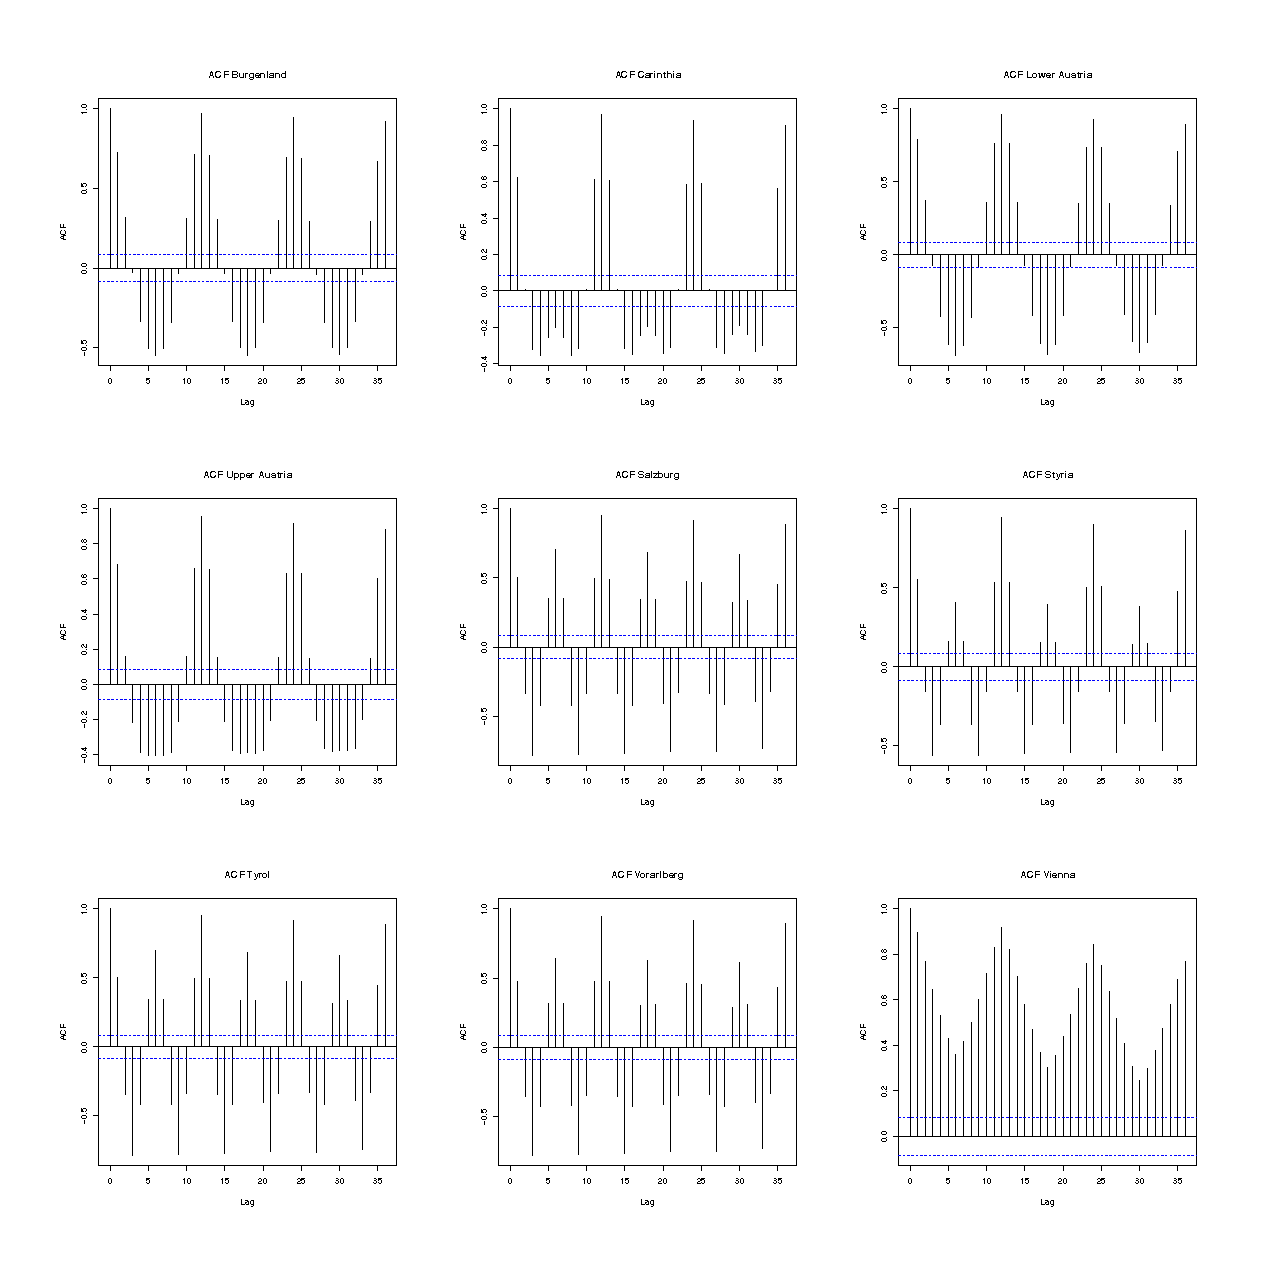
\includegraphics[width=1\textwidth]{images/EA/ACF.pdf}
    \caption{ Autocorrelation functions of raw time series for all nine provinces (the blue dashed lines show the 95\% confidence intervals).}\label{fig:ACFplot}
\end{minipage}
\end{figure} 
\begin{figure}[h!]
\begin{minipage}[b]{1\textwidth}
\centering
    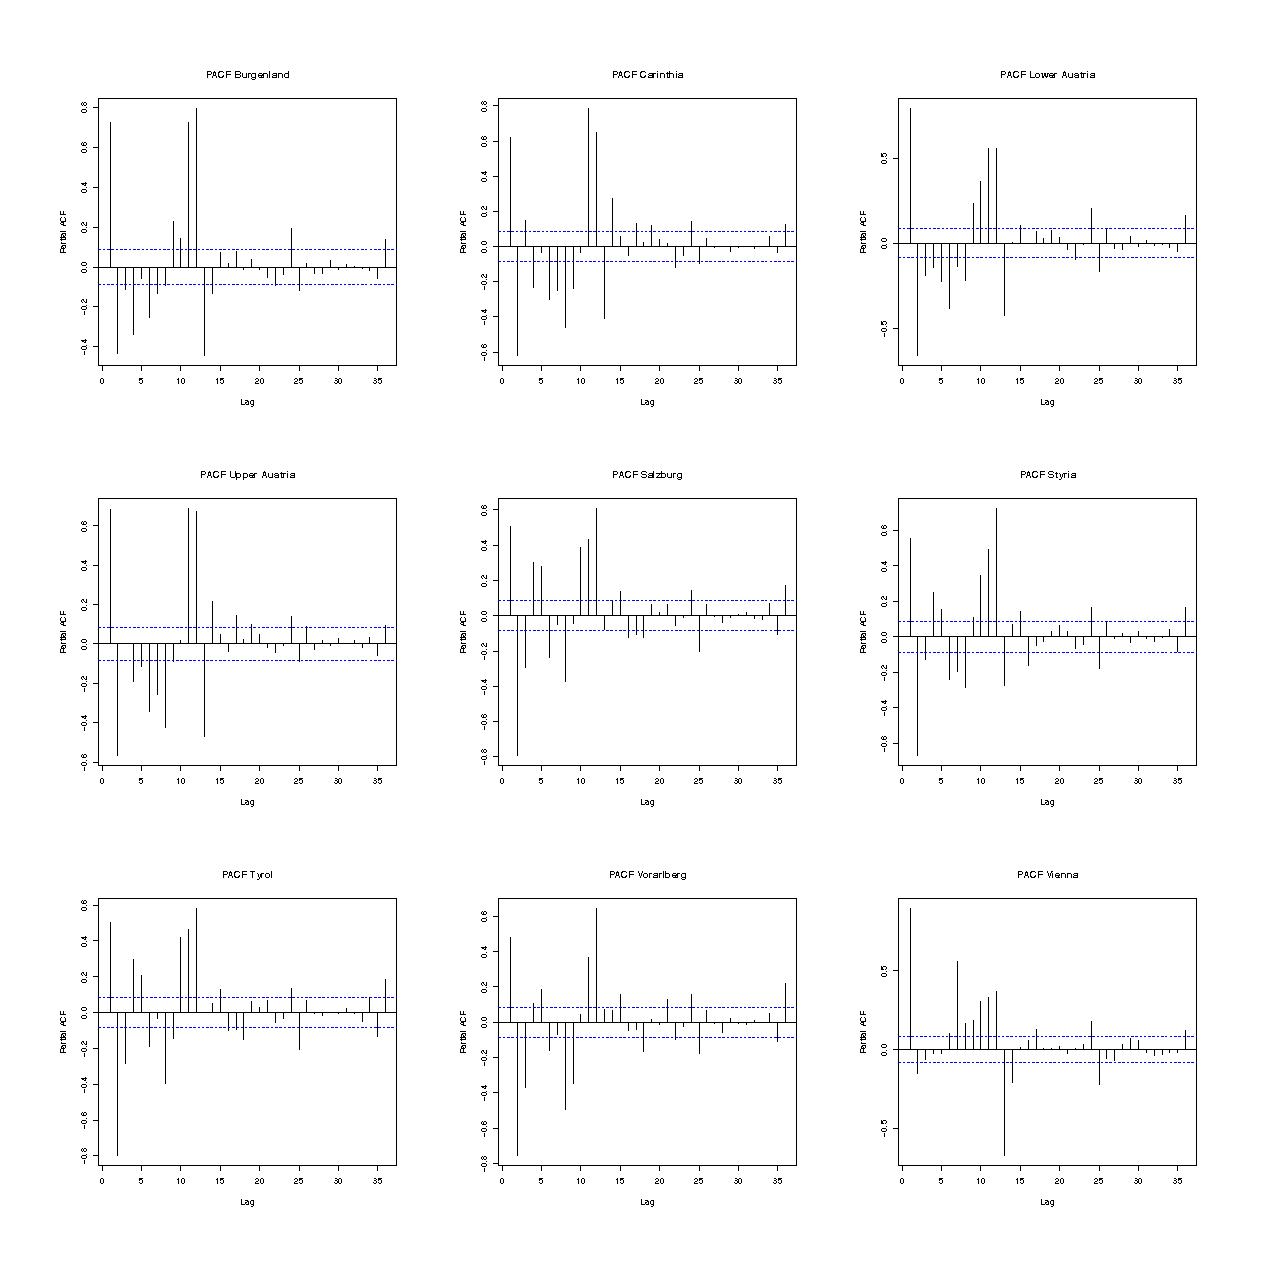
\includegraphics[width=1\textwidth]{images/EA/PACF.pdf}
    \caption{ Partial autocorrelation functions of raw time series for all nine provinces (the blue dashed lines show the 95\% confidence intervals) }\label{fig:PACFplot}
\end{minipage}
\end{figure} 
\newpage
\clearpage
\subsection{Spatial Patterns}
\label{ssec:s_pat}
\subsubsection{Distribution of Stays}
\label{ssec:s_pat_stays}
Figure \ref{fig:hist} shows the histograms of the stays distribution. A marked asymmetry can be seen in Burgenland, Carinthia, Lower Austria and Upper Austria. Two peaks are present in Salzburg, Tyrol and Vorarlberg.
%Figure \ref{fig:hist_12} shows the histograms which reflect a more symmetrical distribution after differencing (lag=12) except for Carinthia which has an outlier over 1e6.
\begin{figure}[H]
\centering
\begin{minipage}[b]{1\textwidth}
\centering
    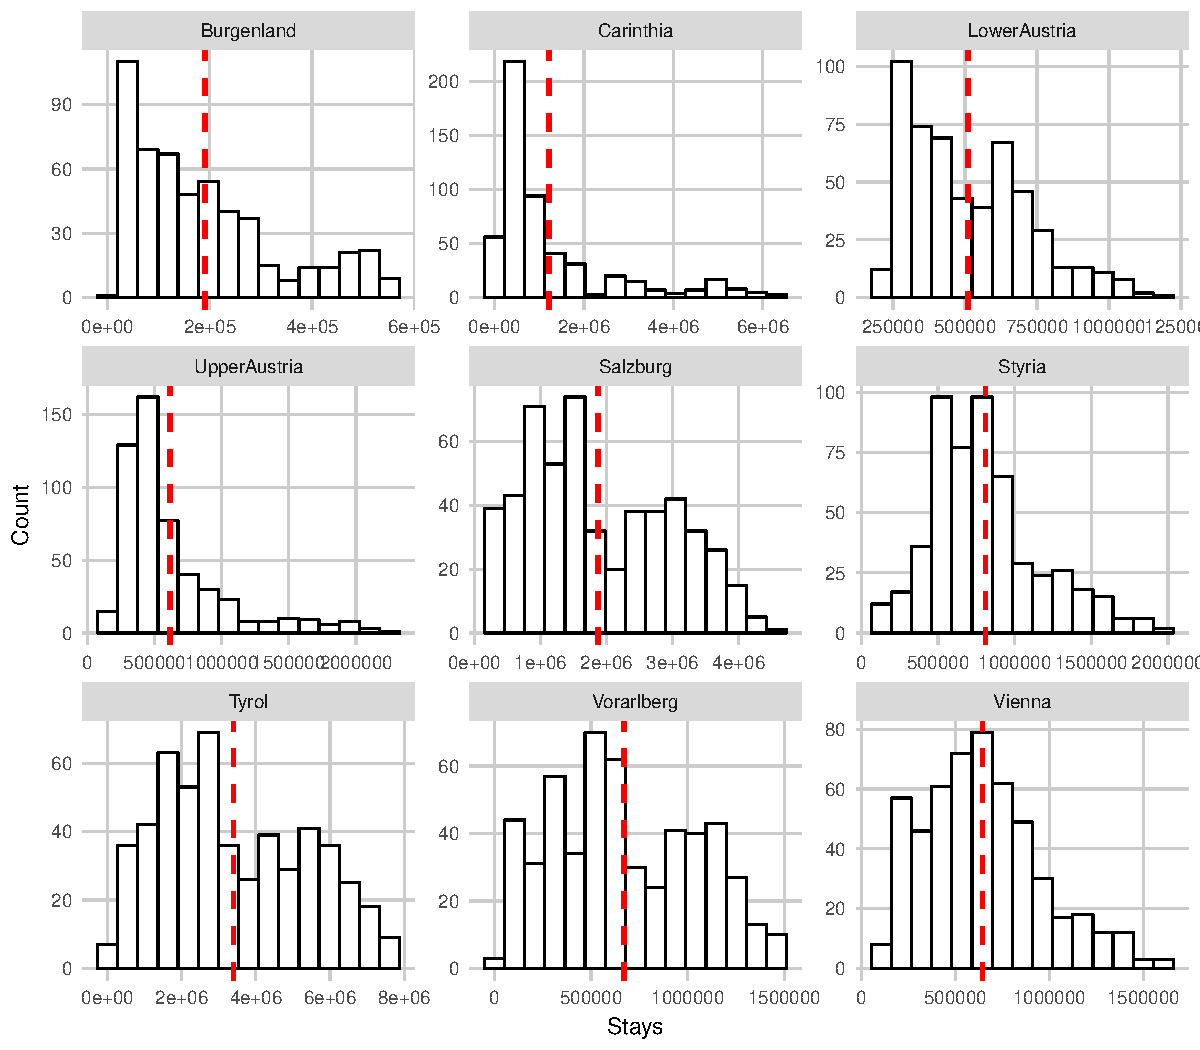
\includegraphics[width=1\textwidth]{images/EA/Hist_ori.pdf}
\caption{Histograms of stays. The red vertical line represents the mean of stays.}
       \label{fig:hist}
\end{minipage}
%\begin{minipage}[b]{0.5\textwidth}
%\centering
%    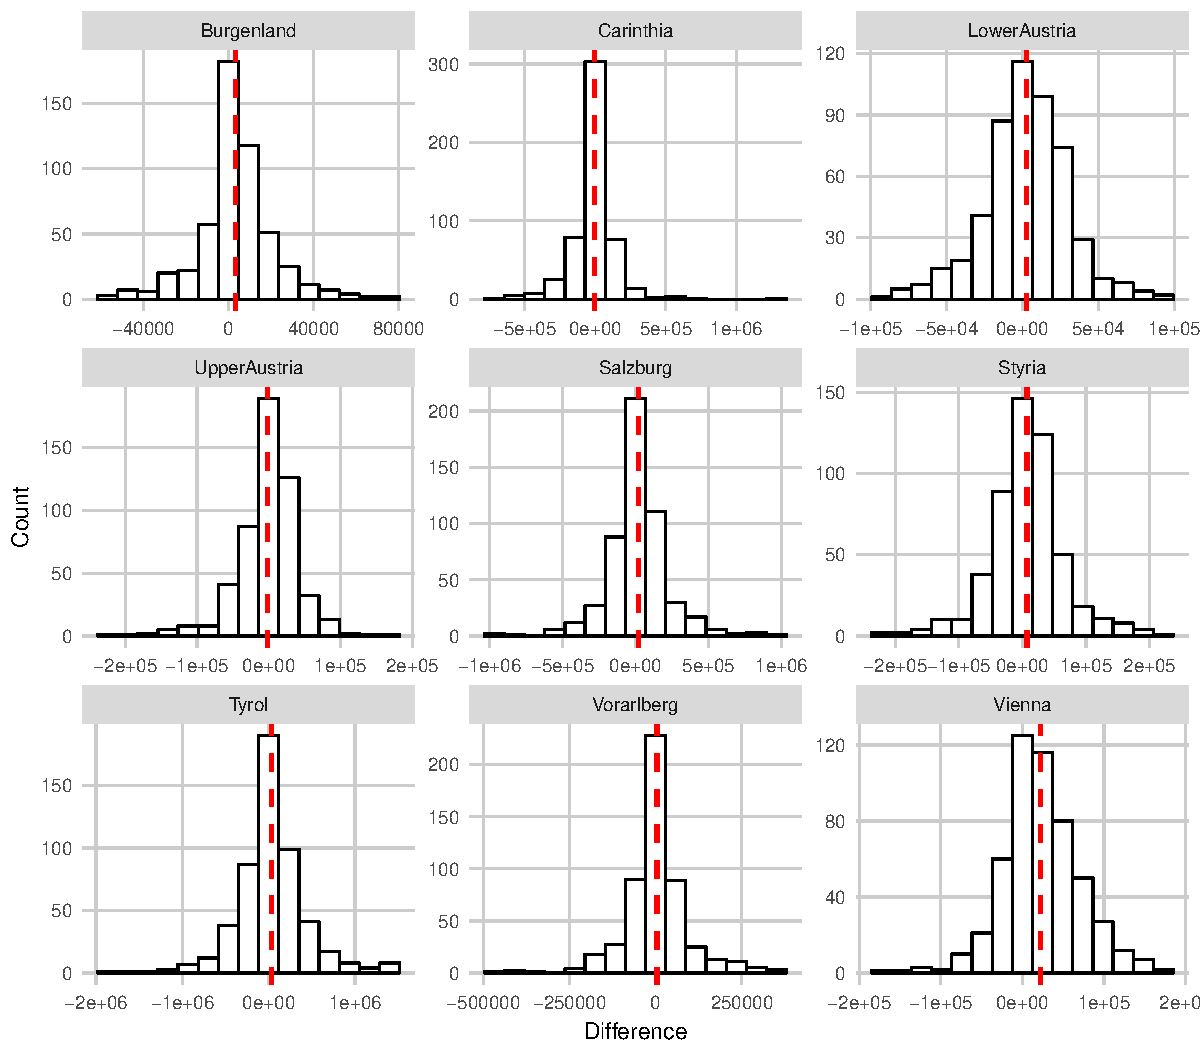
\includegraphics[width=1\textwidth]{Hist_diff_12.pdf}
%    \caption{Histograms of Stays after differencing. The red vertical line represents the mean of difference.}
%       \label{fig:hist_12}
%\end{minipage}
\end{figure} 
\newpage
\subsubsection{Moran's I}
\label{ssec:s_pat_Moran}
Moran’s I is a significant indicator of presence of spatial autocorrelation in the data. This index is estimated for arrivals and stays and is as follows in table \ref{tab:morans_I_glob}.
\begin{longtable}[h!]
{!{\vrule width0.05cm}g!{\vrule width0.05cm}g!{\vrule width0.05cm}g!{\vrule width0.05cm}g!{\vrule width0.05cm}g!{\vrule width0.05cm}g!{\vrule width0.05cm}}
\caption{Comparison of Global Moran's I between monthly tourist arrivals and overnight stays in Austria from 1974-2017 .}
\label{tab:morans_I_glob} \\
\specialrule{0.05cm}{.0cm}{.0cm}
\multicolumn{1}{!{\vrule width0.05cm}c!{\vrule width0.05cm}}
{\bfseries Variable \par} & 
\multicolumn{1}{c!{\vrule width0.05cm}}{\bfseries Moran's I \par} & \multicolumn{1}{c!{\vrule width0.05cm}}{\bfseries Expectation \par} & \multicolumn{1}{c!{\vrule width0.05cm}}{\bfseries Variance \par} &
\multicolumn{1}{c!{\vrule width0.05cm}}{\bfseries p-Value \par} &
\multicolumn{1}{c!{\vrule width0.05cm}}{\bfseries Alternative Hypothesis \par}
\\ 
\specialrule{0.05cm}{.0cm}{.0cm} 
Stays & -0.04715124 & -0.12500000 & 0.03713860 & 0.3431 & greater\\ \specialrule{0.025cm}{.0cm}{.0cm}
\rowcolor{white}Arrivals & -0.07697893 & -0.12500000 & 0.04322940 & 0.4087 & greater \\ \specialrule{0.05cm}{.0cm}{.0cm}
\end{longtable}
\noindent
The p-values in both cases of Moran’s I are not significant. Hence, there is not much spatial autocorrelation and the null hypothesis that the processes are happening due to random chance cannot be rejected. Both Moran's I values are negative, which indicates that there is dispersion rather than clustering. To investigate further, the local Moran's I is calculated for any evidence of spatial autocorrelation at local level (see table \ref{tab:data_Localmoran}).
\begin{longtable}[h!]
{!{\vrule width0.05cm}g!{\vrule width0.05cm}g!{\vrule width0.05cm}g!{\vrule width0.05cm}g!{\vrule width0.05cm}g!{\vrule width0.05cm}g!{\vrule width0.05cm}}
\caption{Local Moran's I for overnight stays, 1974-2017.}
\label{tab:data_Localmoran} \\
\specialrule{0.05cm}{.0cm}{.0cm}
\multicolumn{1}{!{\vrule width0.05cm}c!{\vrule width0.05cm}}
{\bfseries Province \par} & 
\multicolumn{1}{c!{\vrule width0.05cm}}{\bfseries I$_i$ \par} &
\multicolumn{1}{c!{\vrule width0.05cm}}{\bfseries E.I$_i$ \par} &
\multicolumn{1}{c!{\vrule width0.05cm}}{\bfseries Var.I$_i$\par} &
\multicolumn{1}{c!{\vrule width0.05cm}}{\bfseries Z.I$_i$ \par} &
\multicolumn{1}{c!{\vrule width0.05cm}}{\bfseries Pr(z $>$ 0) \par}
\\ 
\specialrule{0.05cm}{.0cm}{.0cm} 
Burgenland & -0.1186 & -0.125 & 0.3514 & 0.0109 & 0.4957\\ \specialrule{0.025cm}{.0cm}{.0cm}
\rowcolor{white}Carinthia & 0.1175 & -0.1250 & 0.1923 &	0.5531 & 0.2901\\ \specialrule{0.025cm}{.0cm}{.0cm}
Lower Austria & -0.3162	& -0.1250 &	0.1302 &	-0.5298 &	0.7019\\ 
\rowcolor{white}Upper Austria& 0.0554 &	-0.1250 & 0.2195 &	0.3850 &	0.3501\\
Salzburg & -0.1909 & -0.1250 &	0.1322 &	-0.1814 &	0.5720 \\
\specialrule{0.025cm}{.0cm}{.0cm}
\rowcolor{white}Styria  & -0.6492 &	-0.1250 & 0.1236 & -1.4911 &	0.9320 \\ \specialrule{0.025cm}{.0cm}{.0cm}
Tyrol & 0.1208 & -0.1250 & 0.2060 & 0.5416 & 0.2940\\ 
\rowcolor{white}Vorarlberg & 0.2596 & -0.1250 & 0.5703 & 0.5093 & 0.3053\\
Vienna & 0.2972 & -0.1250 & 0.5703 & 0.5591 & 0.2880 \\
\specialrule{0.05cm}{.0cm}{.0cm}
\end{longtable}
\noindent
The local Moran's I shows a slight increase in spatial autocorrelation at local level, but still none of the p-values are significant. Mapping the local Moran’s I results (figure \ref{fig:morans_i}) clearly shows presence of spatial clustering and dispersion. The north-eastern part of Austria consisting of Burgenland, Lower Austria, Upper Austria, Styria and Salzburg are forming a cluster of relatively low values, while the south-western part including Carinthia, Tyrol, and Vorarlberg is forming another cluster of high values. The only exception is Vienna, which 
%in spite of being located in the northern part neighbouring the lower value cluster 
has much higher tourist stays compared to its neighbours.    
%in spite of spatial autocorrelation 
%could be the  there are only nine provinces, which might be a insufficient number of data entity to be used for estimating the spatial autocorrelation.
\begin{figure}[H]
\centering
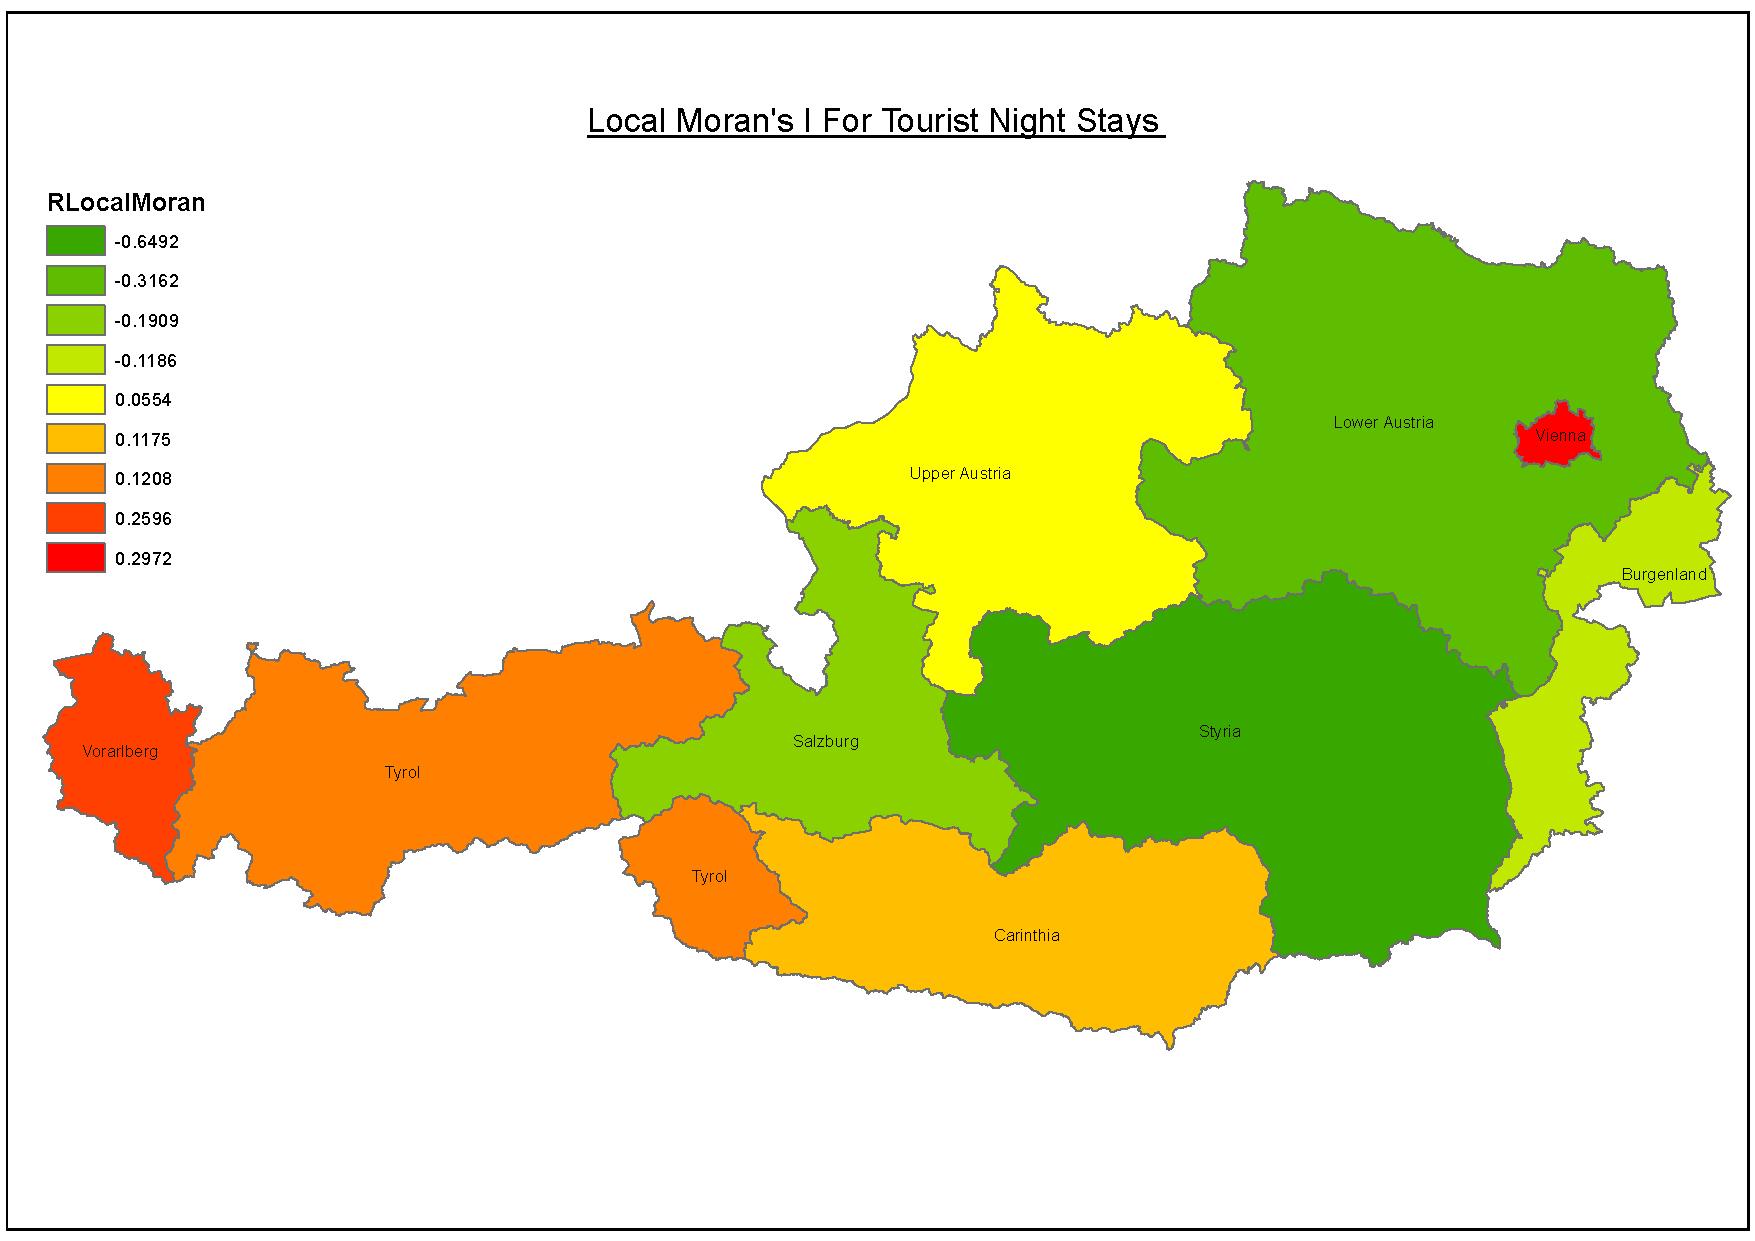
\includegraphics[width=\textwidth]{images/EA/LocalMoranStaysMap.pdf}
\caption{Local Moran's I for overnight stays, 1974-2017}
\label{fig:morans_i}
\end{figure}
\noindent
One issue causing the low estimation of Moran's I could be the insufficient number of data entities (only nine provinces) used for estimating the spatial autocorrelation. One way to find out the presence of spatial autocorrelation and its impact on modelling prediction would be to use a space-time version of one of the machine learning methods by applying various spatial weight matrices and see if there is any significant improvement.  
\clearpage
\subsection{Spatio-Temporal Patterns}
\label{ssec:st_pat}
Similarly to the ACF and PACF their spatio-temporal (ST) equivalents reveal information about spatio-temporal patterns in the data (see figure \ref{fig:ST(P)ACFplot}). As spatial weights the shared border length of a counties neighbours is used (see table \ref{tab:w_borderlen}), although the neighbourhood adjacency first order leads to almost the same result. As only the data from Austria is available, the borders to neigbouring countries are ignored. The STACF at spatial lag 1 shows again a cyclic pattern which seems to be a mixture of all single ACF, thus showing the presence of autocorrelation once again. In the STPACF surprisingly the lags 4, 5 and 9 are significant whereas lag 12 is slightly smaller than the 95 \% confidence interval. 
\\
\\               
\begin{minipage}[h!]{0.98\textwidth}
%\vspace{0.5cm}
\centering
\captionof{table}{Spatial weight matrix weighted by shared border length of touching provinces. All values are normalised by the sum of each row.}
\label{tab:w_borderlen}
\vspace{1.7cm}
\begin{tabular}[h!]{r|ccccccccc}
&
\begin{rotate}{60} Burgenland \end{rotate} &
\begin{rotate}{60} Carinthia \end{rotate} &
\begin{rotate}{60} Lower Austria\end{rotate} &
\begin{rotate}{60} Upper Austria\end{rotate} &
\begin{rotate}{60} Salzburg\end{rotate} &
\begin{rotate}{60} Styria\end{rotate} &
\begin{rotate}{60} Tyrol\end{rotate}&
\begin{rotate}{60} Vorarlberg\end{rotate}&
\begin{rotate}{60} Vienna\end{rotate}\\ \hline 
Burgenland       & 0 & 0  &   0.6076     &   0 & 0 & 0.3924    & 0 & 0 & 0 \\
Carinthia        & 0 & 0  &   0  &   0 & 0.3073    & 0.4643    & 0.2284    & 0 & 0 \\
Lower Austria    & 0.2715 & 0  &   0  &   0.2855    & 0 & 0.2705    & 0 & 0 & 0.1726 \\
Upper Austria    & 0 & 0  &   0.3919     &   0 & 0.3319    & 0.2761    & 0 & 0 & 0 \\
Salzburg        &  0 & 0.2089     &   0  &   0.3138    & 0 & 0.1899    & 0.2873    & 0 & 0 \\
Styria        & 0.1692 & 0.2347     &   0.2609     &   0.1940    & 0.1412    & 0 & 0 & 0 & 0 \\
Tyrol        &0 & 0.2783  &   0  &   0 & 0.5147    & 0 & 0 & 0.2070 & 0 \\
Vorarlberg        & 0 & 0  &   0  &   0 & 0 & 0 & 1 & 0 & 0 \\
Vienna        & 0 & 0  &   1  &   0 & 0 & 0 & 0 & 0 & 0  \\\hline
\end{tabular}
\end{minipage}
\\
\\
\begin{figure}[h!]
\begin{minipage}[b]{1\textwidth}
\centering
    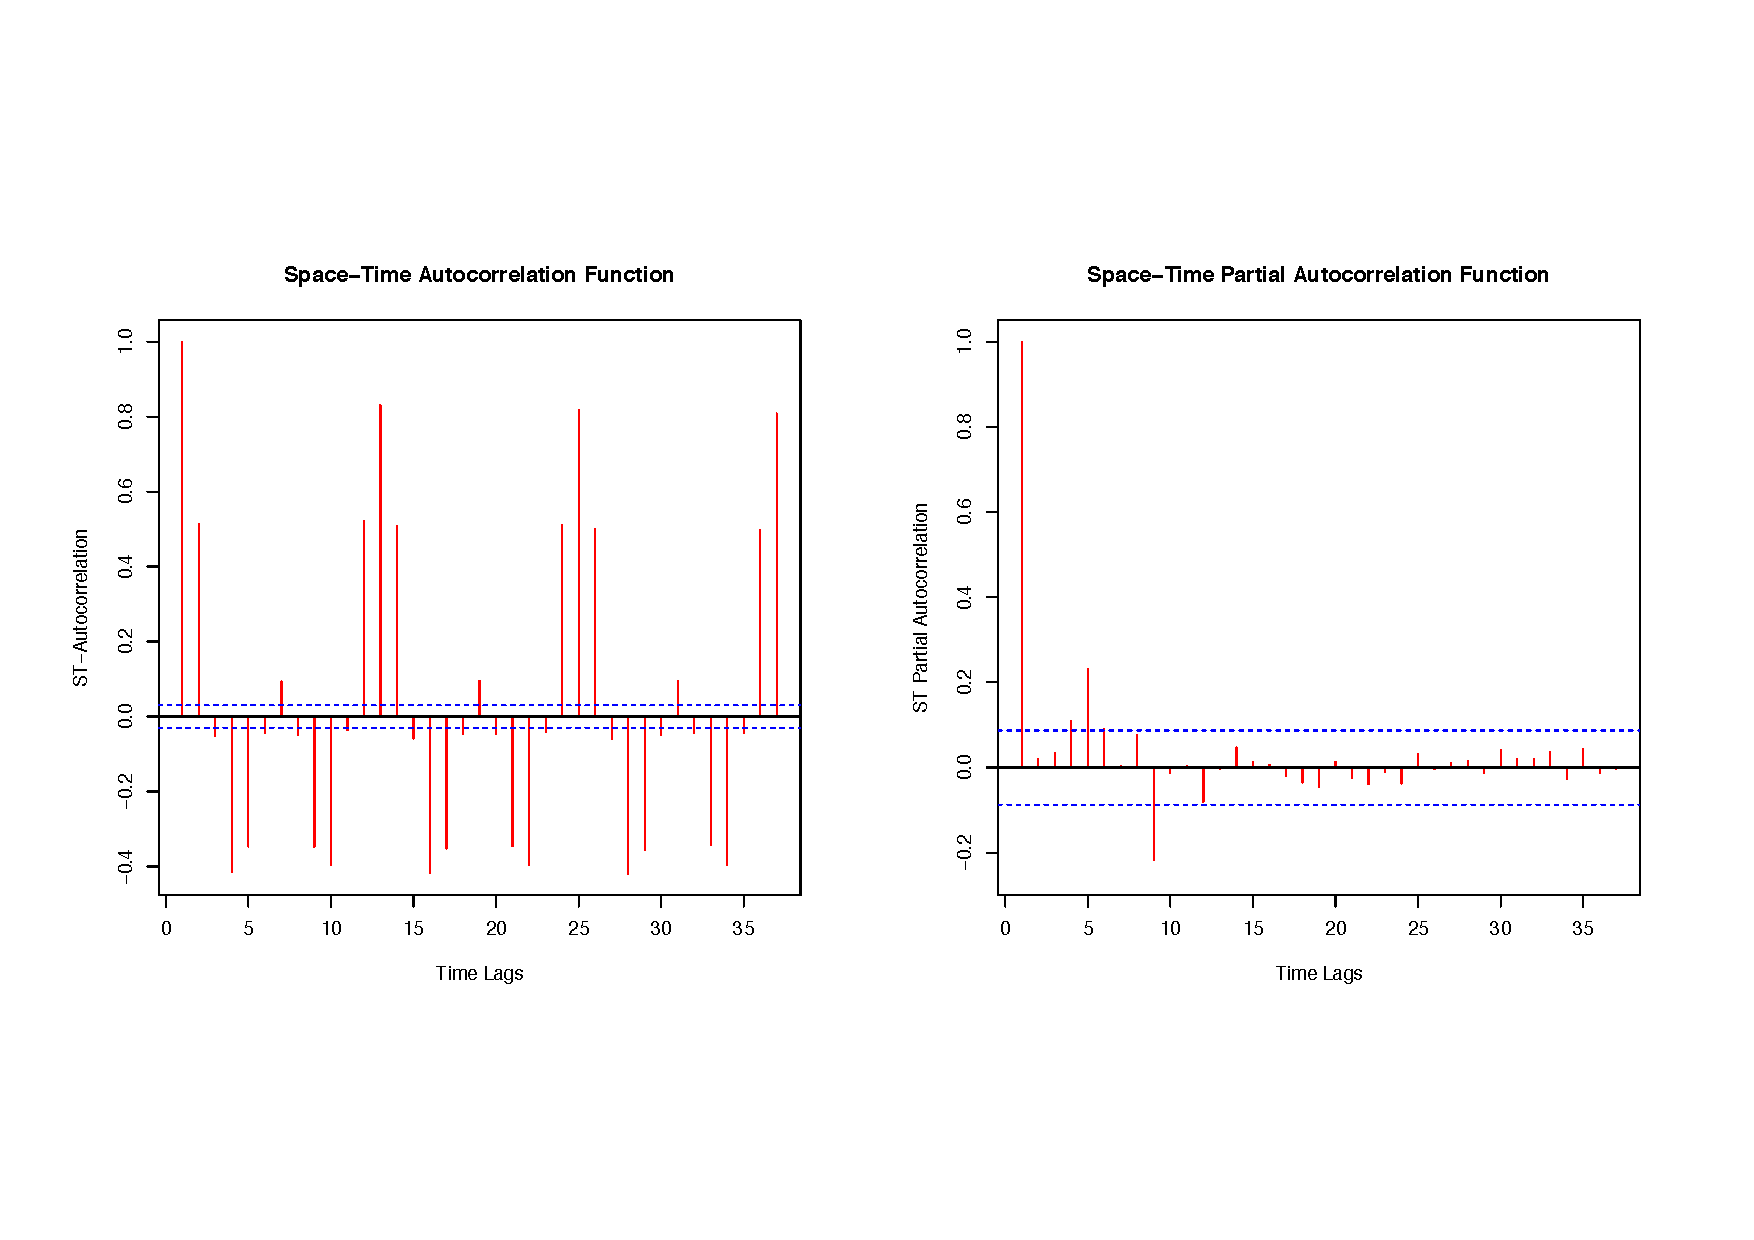
\includegraphics[width=0.9\textwidth]{images/EA/STACF_STPACF.pdf}
    \caption{ Spatio-temporal autocorrelation function and spatio-temporal partial autocorrelation function of raw time series with neighbourhood first order as spatial weights (the blue dashed lines show the 95\% confidence intervals) }\label{fig:ST(P)ACFplot}
\end{minipage}
\end{figure} 
\newpage
\noindent
%Temporal investigations of all provinces point out important properties, which have to be considered for further analysis. Tyrol and Salzburg show a variation in the occurrence of summer/winter peaks. The magnitude between the peaks equalise in the 80's (same amount of stays in summer and winter), but becomes different again (higher peak in winter) towards the end of the time series.  A strong growth in tourist stays is present in Vienna and a decline in Carinthia (see figure \ref{fig:tourist_trend_map}). Arrivals grow much faster than stays, which could be explained with a price decrease for flight tickets and better mobility offers and comfortableness.
Another interesting relation between space and time is illustrated in figure \ref{fig:trend_stays}. Every province shows the increase or decrease of tourist stays based on a linear model. A large positive slope for Tyrol and Vienna implies that throughout the years (from 1973-2017) more and more tourists have visited those provinces or tend to stay longer (assuming the amount of arrivals stays the same). %In contrast, Carinthia is characterised by a remarkable loss in stays. 
Care has to be taken when using those provinces for time series models, where the data needs to be corrected for a trend. If the relation between stays and months is not linear as assumed for the trend reduction, large residuals will affect a proper model training. This implies, that those provinces might be the most difficult to predict.       
\begin{figure}[h!]
\begin{minipage}[b]{1\textwidth}
\centering
    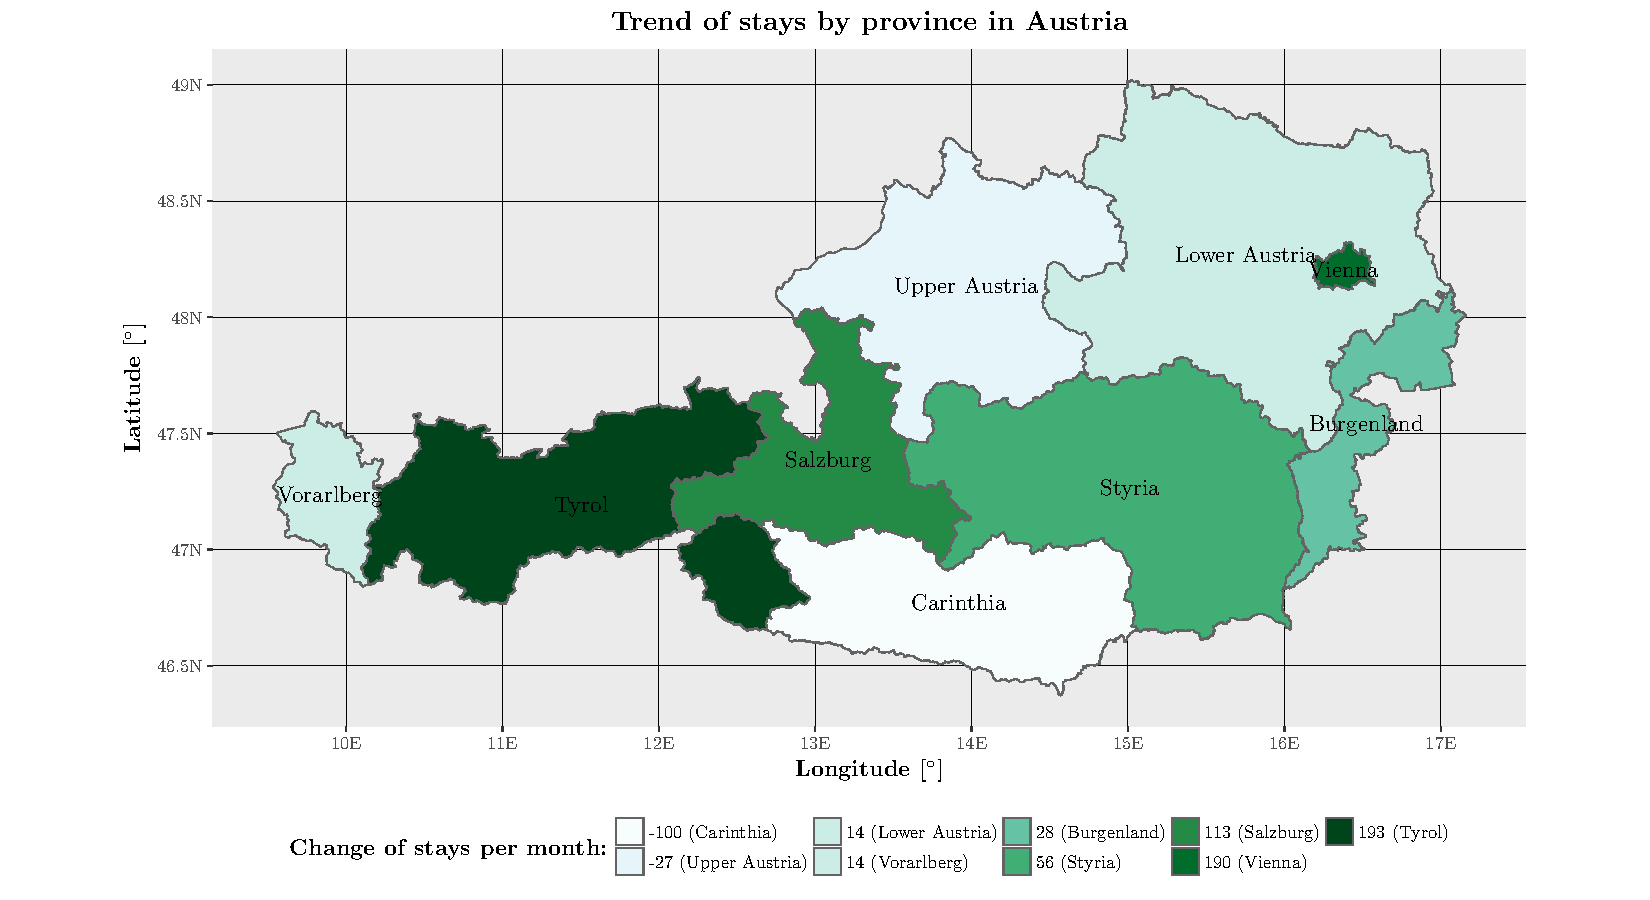
\includegraphics[width=0.9\textwidth]{images/EA/provinces_stays_trend.pdf}
    \caption{Austrian map shows slope value of a line (trend) representing the stays time series for each province from 1973-2017. This means that the depicted values indicate an increase/decrease of tourists per month.}\label{fig:trend_stays}
\label{fig:tourist_trend_map}
\end{minipage}
\end{figure} 
\newpage
\section{Methods}
\label{sec:methods}
Having a focus on regression, all four methods are described and applied on the tourist dataset in the subsequent sections. Each method, \textit{RFR} (subsection \ref{ssec:rfr}), \textit{STARIMA} (subsection \ref{ssec:starima}), \textit{ANN} (subsection \ref{ssec:ann}) and \textit{SVM} (subsection \ref{ssec:svm}), is introduced by a literature review, requires different data pre-processing steps and is applied on the modified data. Finally, all results are shown, which are used for a method comparison in the discussion (see section \ref{sec:disc_and_outl}).  
\subsection{Random Forest Regression (RFR)}
\label{ssec:rfr}
\fancyhead[R]{Methods: RFR}
%Random forest is a (supervised) machine learning method, which offers a usage for classification and regression problems. 
%First basics of the method were mentioned by \cite{ho1995random} as \textit{Random Decision Forest}, who suggests to use multiple trees instead of a single tree. 
%Each tree uses random subspace of the training data opposing the problem of overfitting (strongly present for classification trees) and reducing the generalisation error. This is called bootstrap aggreggation, or \textit{"bagging"}. 
%A different approach is \textit{"boosting"} \cite{boosting}, where weighted \textit{weak learner}s (e.g. single tree) are used to construct a \textit{strong learner} (weighted by wrong predictions of successors). 
The random forest algorithm was designed by Breiman (\cite{breiman2001random}), which unites his original idea of bootstrap aggreggation (\textit{"bagging"}) and an additional randomness in feature selection (\textit{"feature bagging"}). 
%to decrease the correlation between single trees/predictors. 
%Many papers (e.g. \cite{breiman2001random}, \cite{liaw2002classification}, \cite{segal2004machine}, \cite{rf_usage_manual}) point out the usefulness of random forest for regression. 
%A comparison to classification regarding a different methodology will be made in subsection \ref{sssec:meth}.
\subsubsection{Methodology}
\label{sssec:meth}
%\textit{RFR} uses the following steps for training and prediction:
The first step in \textit{RFR} involves a random selection with replacement of the input data for each predictor/feature (\textit{"bagging"}). This ensures that each tree is constructed by using a different bootstrap sample opposing the problem of overfitting 
%(strongly present for classification trees) 
and reducing the generalisation error. On average, about one third of the data is excluded from training from each tree (\textit{"out-of bag" (OOB)} data). \texttt{ntree}\footnote{words written in this style refer to parameters of the \textit{randomForest} package in \textit{R}. For further details see \cite{rf_manual}.} is responsible for the size of the forest.  
%The unused data is called  and is essential for computing error metrics and the variable importance. 
\\
\\
A single tree is built by using a slightly modified \textit{Classification and Regression Trees (CART)} algorithm (\cite{dtl_wiki}). \textit{CART} creates a binary decision tree structure leading to smaller data subsets per node level. At each node an attribute test is applied on data subsets for each feature, partitioning the source data into two subgroups. \textit{RFR} uses \textit{"variance reduction"} to define the "best split" and measures the impurity/difference between the parent and child nodes. All values of each feature are used for testing the impurity of the resulting split. \textit{Residual Sum of Squares (RSS)} is taken to estimate the variance of the elements belonging to one node and the largest difference defines the best split. \textit{Variance reduction} aims to minimise the variance along different node levels, thus ensuring that there are more similar elements in the same regions of the tree. Dominant predictors tend to be selected more often in \textit{CART}, which leads to a higher correlation. Therefore, Breiman suggested to randomly select a subset of predictors to be taken into account for splitting a node (\texttt{mtry}). Moreover, trees are grown to full size (if e.g. \texttt{nodesize} isn't set).
\\
\\
%In random forests not all predictors are chosen to be a possible candidate for the best split.   
%After training has been completed, one can apply the generated random forest on unseen data to predict the variable of interest. 
\textit{RFR} uses the mean of all single tree predictions as a final prediction (\cite{rf_wiki}).   
Furthermore, it offers unbiased error metrics and other useful outputs, for instance the MSE and Pseudo-R$^{2}$ based on \textit{OOB} data and variable importance (\cite{rf_manual}). 
%Both measures are calculated by using the \textit{OOB}-data, which replaces other methods for error estimation like k-fold cross-validation. 
The latter one is computed by averaging \textit{variance reduction} for each predictor. % as a measure of applicability of a variable for prediction. 
%In other words, a predictor which yields a strong decrease in variance is a suitable classifier.     
\\
\\
%\textit{RFR} is mainly dependent on two parameters, namely the number of trees to be grown (\texttt{ntree}) and the number of randomly selected features (\texttt{mtry}). \texttt{ntree} can be set large, since a random forest can't overfit, it is fast, and a higher number leads to an increase in stability (\cite{rf_usage_manual}). \cite{liaw2002classification} suggests to restrict \texttt{ntree} according to the number of predictors (more trees are needed when more predictors are used). Breiman recommends $\texttt{mtry}=p/3$ for regression with $p$ being the number of predictors. It has to be set higher if the input is noisy or there are only a few important predictors in a set of many predictors. Additionally, \texttt{nodesize} is another reasonable parameter to be adjusted ($\texttt{nodesize}=5$). If it is set larger, it causes smaller trees to be grown and increases runtime performance (\cite{rf_usage_manual}).  
\newpage
\subsubsection{Experimental Setup}
\label{sssec:prepro}
%Firstly, the given tourist data required a few pre-processing steps and a definition of useful predictors. 
Various seasonal cycles are an essential feature of the data (see \ref{ssec:t_pat}) being meaningful as explanatory variables. Therefore, stays data was lagged by all 12 months per province using the functions \texttt{t\_embed} and \texttt{st\_embed} \footnote{see practical 5 of STDM}. Additionally, months (e.g. 1, 2, ...., 12) as themselves were also used as input data (\texttt{DateMod}). 
%The distinctiveness and usefulness of each predictor was analysed in respect to variable importance in \textit{RFR}, which will be shown in section \ref{sssec:anal}. 
\\
\\
%Using the modified data
Three different experiments were realised to find the optimal \textit{RFR} model for prediction:% They were set up as follows:    
\begin{enumerate}
\item province-wise training/prediction (\texttt{t\_embed}). 
\item province-wise training/prediction including lagged data of first-order neighbours (\texttt{st\_embed}).
\item training/prediction using stacked province-wise lags. 
\end{enumerate}
To assess the best method from above, some of the default parameters  ($\texttt{ntree}=1000$, $\texttt{mtry}=p/3$\footnote{$p$ equals to the total number of predictors}, $\texttt{nodesize}=5$) were tuned after selecting the best model. 
\subsubsection{Analysis}
\label{sssec:anal}
To get an impression of how the different setups compete against each other, RMSE and R$^{2}$ values are shown in table \ref{tab:t_by_prov}, \ref{tab:st_by_prov} and \ref{tab:t_all}. 
%Additionally, the top five ranked lags (according to variable importance) extend table \ref{tab:t_by_prov} and \ref{tab:st_by_prov}.
%A strong similarity of lags between the provinces is present in table \ref{tab:t_by_prov}. 
In table \ref{tab:t_by_prov}, Lag 12 is clearly the most dominant variable, followed by  lag 9, lag 11, lag 1, lag 6 and lag 3. %For some provinces, the \textit{DateMod} predictor seems to also add some information to the model.   
Table \ref{tab:st_by_prov}, additionally including lagged data from neighbouring provinces, reveals that lag 12, lag 9, lag 6 and lag 3 are the leading predictors. For some provinces (e.g. Vienna) stays from neighbouring countries seem to be a better predictor than the province itself. The error metrics underline a worse model performance when including implicit spatial relations. Vienna has by far the worst R$^{2}$, which is even decreasing for the spatial \textit{RFR}. The RMSE increases remarkably for nearly every province. 
\\
\\
Using a simpler approach of stacking the lagged data, but ignoring any spatiality and province-wise distinction, turns out to be the best performing \textit{RFR} model. In table \ref{tab:t_all}, Vienna is characterised by the most significant improvement and all RMSE's are nearly lowered by half compared to the previous models.  
\newpage
\begin{longtable}[h!]
{!{\vrule width0.05cm}g!{\vrule width0.05cm}g!{\vrule width0.05cm}g!{\vrule width0.05cm}g!{\vrule width0.05cm}g!{\vrule width0.05cm}g!{\vrule width0.05cm}g!{\vrule width0.05cm}g!{\vrule width0.05cm}}
\caption{Top 5 ranked important predictors and error metrics for a province-wise \textit{RFR} model. Green represents the best province, red the worst.}
\label{tab:t_by_prov}\\
\specialrule{0.05cm}{.0cm}{.0cm}
\multicolumn{1}{!{\vrule width0.05cm}c!{\vrule width0.05cm}}{\bfseries Province \par} & 
\multicolumn{1}{c!{\vrule width0.05cm}}{\bfseries RMSE \par} & 
\multicolumn{1}{c!{\vrule width0.05cm}}{\bfseries R$^{2}$ \par} & 
\multicolumn{1}{c!{\vrule width0.05cm}}{\bfseries 1 \par} & \multicolumn{1}{c!{\vrule width0.05cm}}{\bfseries 2 \par} & \multicolumn{1}{c!{\vrule width0.05cm}}{\bfseries 3 \par} &
\multicolumn{1}{c!{\vrule width0.05cm}}{\bfseries 4 \par} &
\multicolumn{1}{c!{\vrule width0.05cm}}{\bfseries 5 \par} \\ 
\specialrule{0.05cm}{.0cm}{.0cm} 
Burgenland  & \cellcolor[HTML]{1a9850} 21197 & \cellcolor[HTML]{d9ef8b} 0.9769 & Lag 12 & Lag 1 & Lag 11 & DateMod & Lag 6 \\ \specialrule{0.025cm}{.0cm}{.0cm}
\rowcolor{white}Carinthia  & \cellcolor[HTML]{ffffbf} 79623 & \cellcolor[HTML]{1a9850} 0.9912 & Lag 9 & Lag 11 & Lag 1 & Lag 12 & Lag 8\\ \specialrule{0.025cm}{.0cm}{.0cm}
Lower Austria  & \cellcolor[HTML]{66bd63} 35635 & \cellcolor[HTML]{fee08b} 0.9703 & Lag 12 & Lag 6 & Lag 11 & Lag 1 & Lag 7  \\ \specialrule{0.025cm}{.0cm}{.0cm}
\rowcolor{white}Upper Austria  & \cellcolor[HTML]{a6d96a} 41249 & \cellcolor[HTML]{66bd63} 0.9819 & Lag 12 & Lag 11 & Lag 8 & Lag 1 & Lag 7  \\ \specialrule{0.025cm}{.0cm}{.0cm}
Salzburg  & \cellcolor[HTML]{fdae61} 226560 & \cellcolor[HTML]{ffffbf} 0.9768 & Lag 12 & Lag 9 & Lag 3 & Lag 6 & DateMod  \\ \specialrule{0.025cm}{.0cm}{.0cm}
\rowcolor{white}Styria  & \cellcolor[HTML]{fee08b} 125486 & \cellcolor[HTML]{f46d43} 0.9208 & Lag 12 & Lag 9 & Lag 3 & Lag 11 & Lag 1  \\ \specialrule{0.025cm}{.0cm}{.0cm}
Tyrol  & \cellcolor[HTML]{d73027} 337781 & \cellcolor[HTML]{a6d96a} 0.9818 & Lag 12 & Lag 9 & Lag 3 & Lag 6 & DateMod   \\ \specialrule{0.025cm}{.0cm}{.0cm}
\rowcolor{white}Vienna  & \cellcolor[HTML]{f46d43} 231508 & \cellcolor[HTML]{d73027} 0.7848 & Lag 12 & Lag 1 & Lag 10 & Lag 11 & Lag 2  \\ \specialrule{0.025cm}{.0cm}{.0cm}
Vorarlberg  & \cellcolor[HTML]{d9ef8b} 71982 & \cellcolor[HTML]{fdae61} 0.9695 & Lag 12 & Lag 9 & Lag 3 & Lag 6 & DateMod   \\ \specialrule{0.05cm}{.0cm}{.0cm}
\end{longtable}
\begin{longtable}[h!]
{!{\vrule width0.05cm}g!{\vrule width0.05cm}g!{\vrule width0.05cm}g!{\vrule width0.05cm}g!{\vrule width0.05cm}g!{\vrule width0.05cm}g!{\vrule width0.05cm}g!{\vrule width0.05cm}g!{\vrule width0.05cm}}
\caption{Top 5 ranked important predictors and error metrics for a province-wise spatial \textit{RFR} model. Lags are related to provinces in brackets (either first-order neighbours or the province itself). Green represents the best province, red the worst.}
\label{tab:st_by_prov}\\
\specialrule{0.05cm}{.0cm}{.0cm}
\multicolumn{1}{!{\vrule width0.05cm}c!{\vrule width0.05cm}}{\bfseries Province \par} & 
\multicolumn{1}{c!{\vrule width0.05cm}}{\bfseries RMSE \par} & 
\multicolumn{1}{c!{\vrule width0.05cm}}{\bfseries R$^{2}$ \par} & 
\multicolumn{1}{c!{\vrule width0.05cm}}{\bfseries 1 \par} & \multicolumn{1}{c!{\vrule width0.05cm}}{\bfseries 2 \par} & \multicolumn{1}{c!{\vrule width0.05cm}}{\bfseries 3 \par} &
\multicolumn{1}{c!{\vrule width0.05cm}}{\bfseries 4 \par} &
\multicolumn{1}{c!{\vrule width0.05cm}}{\bfseries 5 \par} \\ 
\specialrule{0.05cm}{.0cm}{.0cm} 
Burgenland  & \cellcolor[HTML]{1a9850} 22348.0 & \cellcolor[HTML]{66bd63} 0.9798 & \begin{tabular}[c]{@{}l@{}}Lag 12 \\ (L. Aus.) \end{tabular} & \begin{tabular}[c]{@{}l@{}} Lag 11 \\(L. Aus.) \end{tabular} & \begin{tabular}[c]{@{}l@{}} Lag 9 \\ (Styria) \end{tabular} & \begin{tabular}[c]{@{}l@{}} Lag 1 \\ (L. Aus.) \end{tabular} & \begin{tabular}[c]{@{}l@{}} Lag 9 \\ (L. Aus.) \end{tabular}  \\ \specialrule{0.025cm}{.0cm}{.0cm}
\rowcolor{white}Carinthia  & \cellcolor[HTML]{fee08b} 159818.0 & \cellcolor[HTML]{d9ef8b} 0.9770 & \begin{tabular}[c]{@{}l@{}}Lag 12 \\ (Salzburg) \end{tabular} & \begin{tabular}[c]{@{}l@{}} Lag 12 \\(Carinthia) \end{tabular} & \begin{tabular}[c]{@{}l@{}} Lag 12 \\ (Tyrol) \end{tabular} & \begin{tabular}[c]{@{}l@{}} Lag 9 \\ (Styria) \end{tabular} & \begin{tabular}[c]{@{}l@{}} Lag 9 \\ (Tyrol) \end{tabular}\\ \specialrule{0.025cm}{.0cm}{.0cm}
Lower Austria  & \cellcolor[HTML]{a6d96a} 35391.0 & \cellcolor[HTML]{ffffbf} 0.9764 & \begin{tabular}[c]{@{}l@{}}Lag 12 \\ (U. Aus.) \end{tabular} & \begin{tabular}[c]{@{}l@{}} Lag 12 \\(L. Aus.) \end{tabular} & \begin{tabular}[c]{@{}l@{}} Lag 6 \\ (U. Aus.) \end{tabular} & \begin{tabular}[c]{@{}l@{}} Lag 11 \\ (L. Aus.) \end{tabular} & \begin{tabular}[c]{@{}l@{}} Lag 1 \\ (U. Aus.) \end{tabular}  \\ \specialrule{0.025cm}{.0cm}{.0cm}
\rowcolor{white}Upper Austria  & \cellcolor[HTML]{66bd63} 31813.0 & \cellcolor[HTML]{1a9850} 0.9864 & \begin{tabular}[c]{@{}l@{}}Lag 12 \\ (Salzburg) \end{tabular} & \begin{tabular}[c]{@{}l@{}} Lag 12 \\(L. Aus.) \end{tabular} & \begin{tabular}[c]{@{}l@{}} Lag 12 \\ (U. Aus.) \end{tabular} & \begin{tabular}[c]{@{}l@{}} Lag 9 \\ (Styria) \end{tabular} & \begin{tabular}[c]{@{}l@{}} Lag 11 \\ (L. Aus.) \end{tabular}  \\ \specialrule{0.025cm}{.0cm}{.0cm}
Salzburg  & \cellcolor[HTML]{fdae61} 245599 & \cellcolor[HTML]{fee08b} 0.9720 & \begin{tabular}[c]{@{}l@{}}Lag 12 \\ (Styria) \end{tabular} & \begin{tabular}[c]{@{}l@{}} Lag 9 \\(Styria) \end{tabular} & \begin{tabular}[c]{@{}l@{}} Lag 3 \\ (Styria) \end{tabular} & \begin{tabular}[c]{@{}l@{}} Lag 3 \\ (Tyrol) \end{tabular} & \begin{tabular}[c]{@{}l@{}} Lag 6 \\ (Styria) \end{tabular}  \\ \specialrule{0.025cm}{.0cm}{.0cm}
\rowcolor{white}Styria  & \cellcolor[HTML]{ffffbf} 127284.0 & \cellcolor[HTML]{f46d43} 0.9476 & \begin{tabular}[c]{@{}l@{}}Lag 12 \\ (L. Aus.) \end{tabular} & \begin{tabular}[c]{@{}l@{}} Lag 12 \\(Carinthia) \end{tabular} & \begin{tabular}[c]{@{}l@{}} Lag 12 \\ (Salzburg) \end{tabular} & \begin{tabular}[c]{@{}l@{}} Lag 12 \\ (Styria) \end{tabular} & \begin{tabular}[c]{@{}l@{}} Lag 12 \\ (U. Aus.) \end{tabular}  \\ \specialrule{0.025cm}{.0cm}{.0cm}
Tyrol  & \cellcolor[HTML]{f46d43} 366814.0 & \cellcolor[HTML]{a6d96a} 0.9778 & \begin{tabular}[c]{@{}l@{}}Lag 12 \\ (Vorarlb.) \end{tabular} & \begin{tabular}[c]{@{}l@{}} Lag 9 \\(Vorarlb.) \end{tabular} & \begin{tabular}[c]{@{}l@{}} Lag 3 \\ (Tirol) \end{tabular} & \begin{tabular}[c]{@{}l@{}} Lag 3 \\ (Vorarlb.) \end{tabular} & \begin{tabular}[c]{@{}l@{}} Lag 6 \\ (Vorarlb.) \end{tabular}  \\ \specialrule{0.025cm}{.0cm}{.0cm}
\rowcolor{white}Vienna  & \cellcolor[HTML]{d73027} 387520.0 & \cellcolor[HTML]{d73027} 0.7269 & \begin{tabular}[c]{@{}l@{}}Lag 6 \\ (L. Aus.) \end{tabular} & \begin{tabular}[c]{@{}l@{}} Lag 5 \\(L. Aus.) \end{tabular} & \begin{tabular}[c]{@{}l@{}} Lag 12 \\ (L. Aus.) \end{tabular} & \begin{tabular}[c]{@{}l@{}} Lag 10 \\ (L. Aus.) \end{tabular} & \begin{tabular}[c]{@{}l@{}} Lag 2 \\ (L. Aus.) \end{tabular}\\ \specialrule{0.025cm}{.0cm}{.0cm}
Vorarlberg  & \cellcolor[HTML]{d9ef8b} 90221.0 & \cellcolor[HTML]{fdae61} 0.9590 & \begin{tabular}[c]{@{}l@{}}Lag 12 \\ (Vorarlb.) \end{tabular} & \begin{tabular}[c]{@{}l@{}} Lag 3 \\(Tirol) \end{tabular} & \begin{tabular}[c]{@{}l@{}} Lag 9 \\ (Vorarlb.) \end{tabular} & \begin{tabular}[c]{@{}l@{}} Lag 3 \\ (Vorarlb.) \end{tabular} & \begin{tabular}[c]{@{}l@{}} Lag 6 \\ (Vorarlb.) \end{tabular}   \\ \specialrule{0.05cm}{.0cm}{.0cm}
\end{longtable}
\begin{longtable}[h!]
{!{\vrule width0.05cm}g!{\vrule width0.05cm}g!{\vrule width0.05cm}g!{\vrule width0.05cm}g!{\vrule width0.05cm}g!{\vrule width0.05cm}g!{\vrule width0.05cm}g!{\vrule width0.05cm}g!{\vrule width0.05cm}g!{\vrule width0.05cm}g!{\vrule width0.05cm}}
\caption{Error metrics for a \textit{RFR} model trained on stacked province-wise lagged data. Green represents the best province, red the worst.}
\label{tab:t_all}\\
\specialrule{0.05cm}{.0cm}{.0cm}
\multicolumn{1}{!{\vrule width0.05cm}c!{\vrule width0.05cm}}{\bfseries  \par} & \multicolumn{1}{c!{\vrule width0.05cm}}{\bfseries \begin{tabular}[c]{@{}l@{}}Burgen-\\land \end{tabular}\par} & 
\multicolumn{1}{c!{\vrule width0.05cm}}{\bfseries Carinthia \par} & 
\multicolumn{1}{c!{\vrule width0.05cm}}{\bfseries \begin{tabular}[c]{@{}l@{}}Lower \\ Austria \end{tabular} \par} & 
\multicolumn{1}{c!{\vrule width0.05cm}}{\bfseries \begin{tabular}[c]{@{}l@{}}Upper \\ Austria \end{tabular} \par} & \multicolumn{1}{c!{\vrule width0.05cm}}{\bfseries \begin{tabular}[c]{@{}l@{}} Salz-\\burg \end{tabular} \par} & \multicolumn{1}{c!{\vrule width0.05cm}}{\bfseries Styria \par} &
\multicolumn{1}{c!{\vrule width0.05cm}}{\bfseries Tyrol \par} &
\multicolumn{1}{c!{\vrule width0.05cm}}{\bfseries Vienna \par} &
\multicolumn{1}{c!{\vrule width0.05cm}}{\bfseries \begin{tabular}[c]{@{}l@{}} Vorarl-\\berg\end{tabular} \par} \\ 
\specialrule{0.05cm}{.0cm}{.0cm} 
{\bfseries RMSE \par} & \cellcolor[HTML]{1a9850} 15913 & \cellcolor[HTML]{fee08b} 73530 & \cellcolor[HTML]{66bd63} 19889 & \cellcolor[HTML]{a6d96a} 29487 & \cellcolor[HTML]{f46d43} 173263 & \cellcolor[HTML]{ffffbf} 71818 & \cellcolor[HTML]{d73027} 317590 & \cellcolor[HTML]{fdae61} 91999 & \cellcolor[HTML]{d9ef8b} 69337 \\ \specialrule{0.025cm}{.0cm}{.0cm}
\rowcolor{white}{\bfseries R$^{2}$ \par} & \cellcolor[HTML]{ffffbf} 0.9809 & \cellcolor[HTML]{1a9850} 0.9926 & \cellcolor[HTML]{d9ef8b} 0.9810 & \cellcolor[HTML]{66bd63} 0.9846 & \cellcolor[HTML]{fee08b} 0.9786 & \cellcolor[HTML]{f46d43} 0.9637 & \cellcolor[HTML]{a6d96a} 0.9812 & \cellcolor[HTML]{d73027} 0.9369 & \cellcolor[HTML]{fdae61} 0.9681  \\ 
\specialrule{0.05cm}{.0cm}{.0cm}
\end{longtable}
\newpage
\noindent
To be able to detect the most important explanatory variables for the finally used method, variable importance was analysed (figure \ref{fig:varimp_t}). $\texttt{ntree}$ was set to 1000, since a lot of trees are necessary to get a stable estimate of variable importance (\cite{liaw2002classification}).
\begin{figure}[h!]
\centering
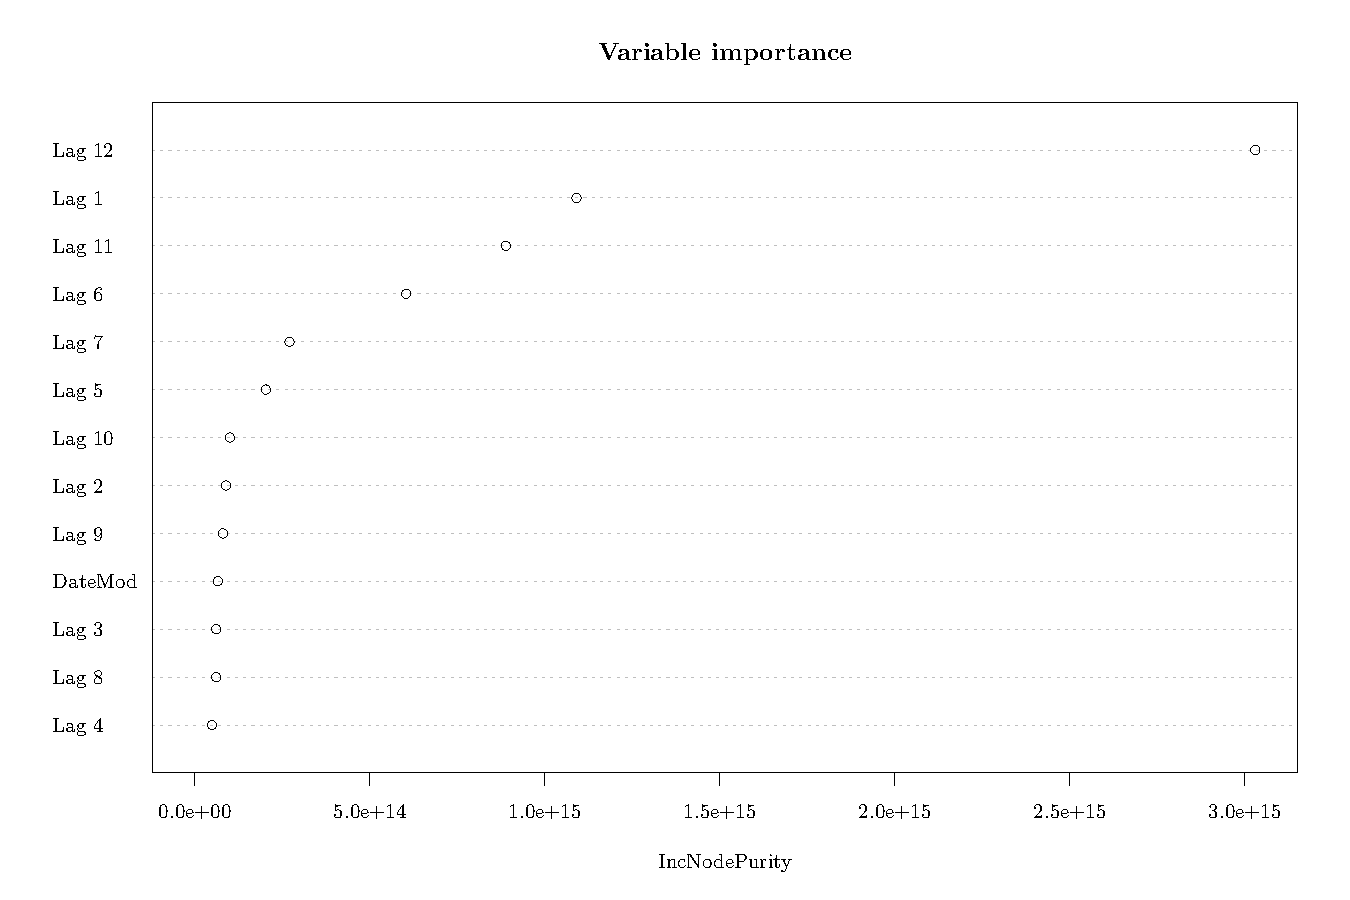
\includegraphics[width=0.9\textwidth]{images/RFR/varimp_t.pdf}
    \caption{Variable importance of the third \textit{RFR} method including lagged stays data and \textit{DateMod}.}
    \label{fig:varimp_t}
\end{figure}
\\
\\
According to figure \ref{fig:varimp_t}, it was decided to take lag 12, lag 11, lag 6 and lag 1 as predictors, since those variables seem to explain stays well enough (replicated conclusion of subsection \ref{ssec:t_pat}). Moreover, less predictors yield a lower runtime.
\\
\\
The next step is dedicated to improve the performance by tuning the mentioned model parameters of the third \textit{RFR} model. Firstly, 5-fold cross-validation was applied to determine the optimal \texttt{ntree}. A %different error metric would be the MSE of the residuals provided by \textit{randomForest}, but a 
reliable error estimate can only be achieved by a higher \texttt{ntree} (more averaged predictions). Thus, cross validation is therefore thought to be more suitable, when investigating different values for \texttt{ntree}. The behaviour of runtime and prediction error depending on \texttt{ntree} can be seen in figure \ref{fig:ntrees}. The prediction error has its lowest value around $\texttt{ntree}=800$ and the relation between runtime and \texttt{ntree} is approximately linear.
%, which underlines Breiman's statement to not be sparse with growing the forest (\cite{rf_usage_manual}).
\newline
\begin{figure}[h!]
\centering
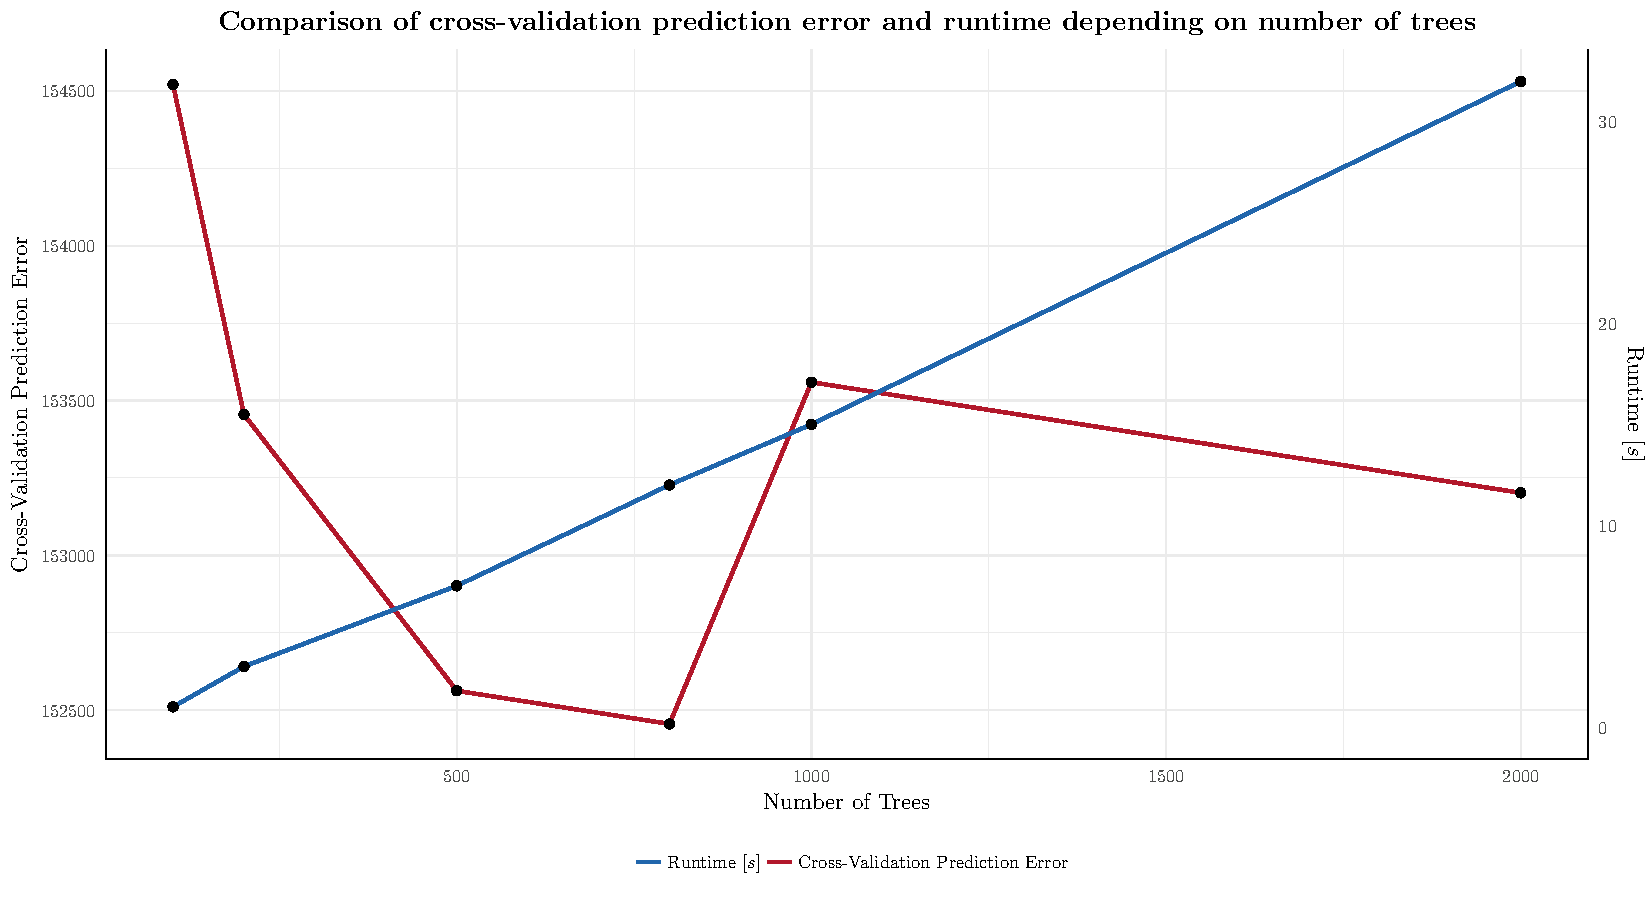
\includegraphics[width=0.9\textwidth]{images/RFR/ntrees.pdf}
    \caption{Runtime and cross-validation error comparison in relation to the number of trees \texttt{ntree}.}
    \label{fig:ntrees}
\end{figure}
\newpage
\noindent
%Secondly, pseudo-R$^2$ is used to optimise the remaining parameters \texttt{mtry} and \texttt{nodesize}. 
Secondly, figure \ref{fig:mtry} and \ref{fig:nodesize} demonstrate that $\texttt{mtry}=2$ and $\texttt{nodesize}=2$ are the best choices having the highest pseudo-R$^2$, which shows the importance of \textit{"feature bagging"} for the former one. %Moreover, 
%figure \ref{fig:mtry} shows the , since 
%$\texttt{mtry}=2$ leads to better results than $\texttt{mtry}=4$ ($=p$).  
\begin{figure}[h!]
\centering
\begin{minipage}[h!]{0.45\textwidth}
\centering
    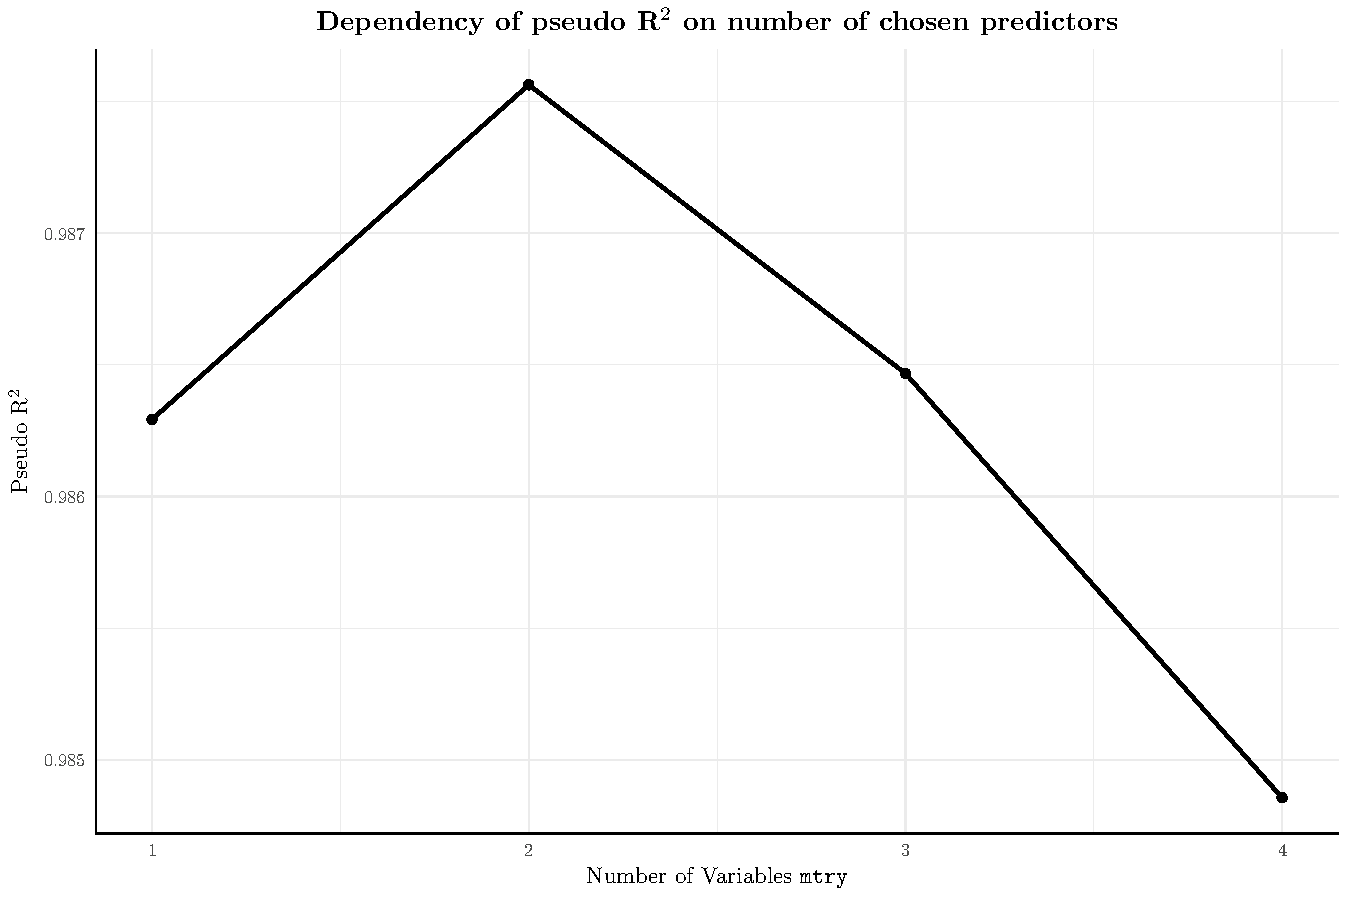
\includegraphics[width=1\textwidth]{images/RFR/mtry.pdf}
    \caption{Performance dependency on number of predictors randomly selected (\texttt{mtry}).}
        \label{fig:mtry}
\end{minipage}
\hspace{0.5cm}
\begin{minipage}[h!]{0.45\textwidth}
\centering
    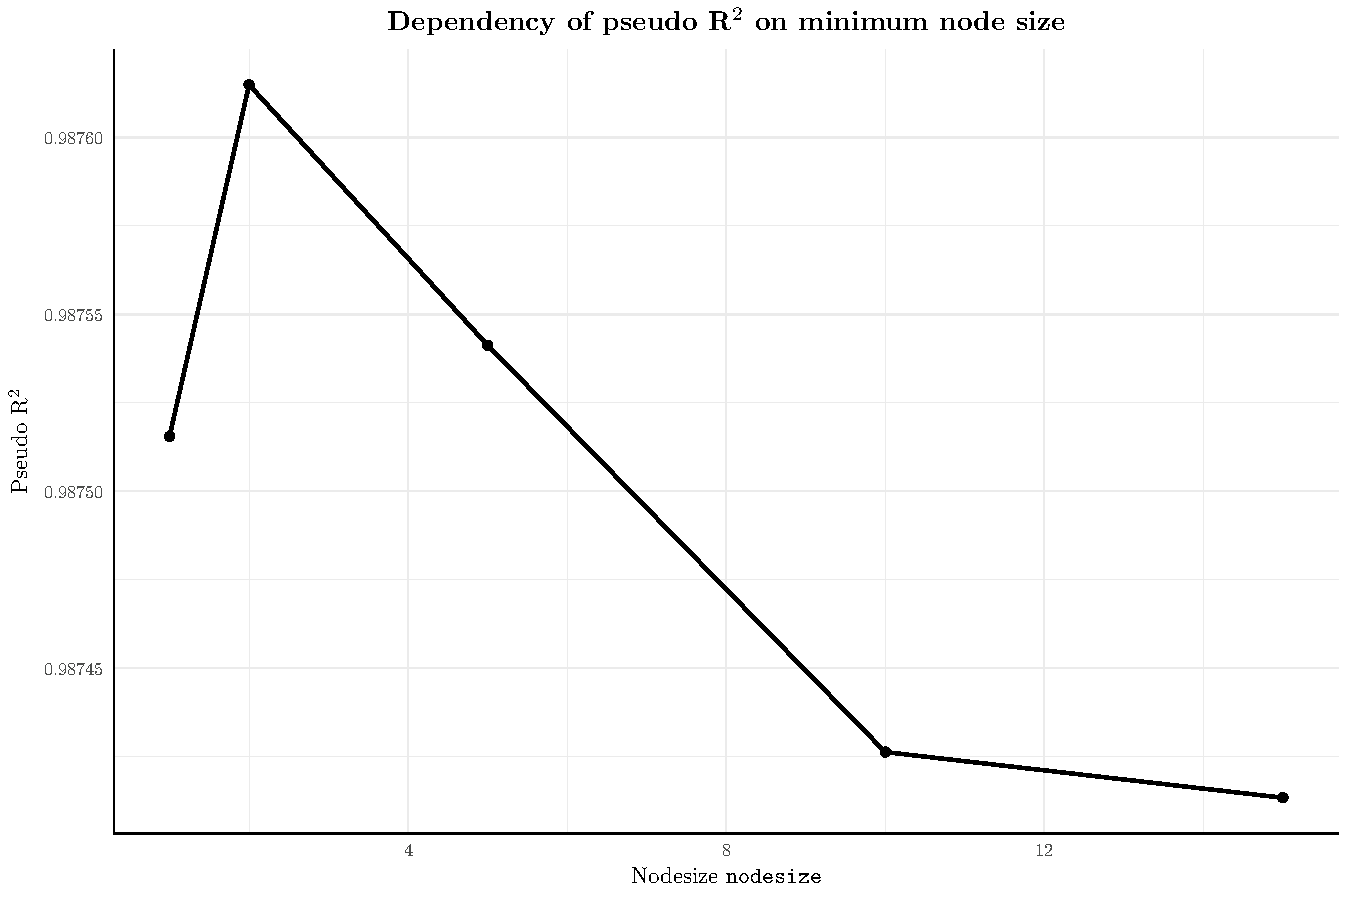
\includegraphics[width=1\textwidth]{images/RFR/nodesize.pdf}
    \caption{Performance dependency on minimum size of terminal nodes (\texttt{nodesize}).}
        \label{fig:nodesize}
\end{minipage}
\end{figure} 
\newpage
\subsubsection{Results}
\label{sssec:res}
Using the optimised parameters and predictors, the error metrics in table \ref{tab:rfr_final_stats} could be achieved.  
\begin{longtable}[h!]
{!{\vrule width0.05cm}g!{\vrule width0.05cm}g!{\vrule width0.05cm}g!{\vrule width0.05cm}g!{\vrule width0.05cm}g!{\vrule width0.05cm}g!{\vrule width0.05cm}g!{\vrule width0.05cm}g!{\vrule width0.05cm}}
\caption{Final error metrics resulting from a \textit{RFR} prediction comprising tuned model parameters. Green represents the best province, red the worst.}
\label{tab:rfr_final_stats}\\
\specialrule{0.05cm}{.0cm}{.0cm}
\multicolumn{1}{!{\vrule width0.05cm}c!{\vrule width0.05cm}}{\bfseries Province \par} & 
\multicolumn{1}{c!{\vrule width0.05cm}}{\bfseries Bias \par} & 
\multicolumn{1}{c!{\vrule width0.05cm}}{\bfseries RMSE \par} & 
\multicolumn{1}{c!{\vrule width0.05cm}}{\bfseries NRMSE \par} & 
\multicolumn{1}{c!{\vrule width0.05cm}}{\bfseries Std. Ratio \par} & \multicolumn{1}{c!{\vrule width0.05cm}}{\bfseries \begin{tabular}[c]{@{}l@{}}Pearson \\ Correlation \end{tabular} \par} & \multicolumn{1}{c!{\vrule width0.05cm}}{\bfseries R$^{2}$ \par} &
\multicolumn{1}{c!{\vrule width0.05cm}}{\bfseries \begin{tabular}[c]{@{}l@{}}Spearman \\ Correlation \end{tabular} \par} \\ 
\specialrule{0.05cm}{.0cm}{.0cm} 
%Burgenland & 707 & 18130 &0.0727 & 0.9967 & 0.9875 & 0.9752 & 0.9741 \\ \specialrule{0.025cm}{.0cm}{.0cm}
%\rowcolor{white}Carinthia & 6286 & 79950 & 0.0760 & 1.0182 & 0.9956 & 0.9913 &
%0.9895\\ \specialrule{0.025cm}{.0cm}{.0cm}
%Lower Austria & -855 & 23383 & 0.0410 & 1.0157 &  0.9867 & 0.9737 & 0.9813  \\ \specialrule{0.025cm}{.0cm}{.0cm}
%\rowcolor{white}Upper Austria & 3726 & 31862 & 0.0526 & 1.0318 & 0.9896 & 0.9794 & 0.9703  \\ \specialrule{0.025cm}{.0cm}{.0cm} Salzburg & 30070 & 204958 & 0.0951 & 1.0596 & 0.9855 & 0.9713 & 0.9767 \\ \specialrule{0.025cm}{.0cm}{.0cm}
%\rowcolor{white}Styria & 628 & 67876 & 0.0697 & 1.0569 & 0.9772 & 0.9550 & 0.9768 \\ \specialrule{0.025cm}{.0cm}{.0cm}
%Tyrol & 54958 & 318733 & 0.0853 & 1.0703 & 0.9892 & 0.9786 & 0.9864  \\ \specialrule{0.025cm}{.0cm}{.0cm}
%\rowcolor{white}Vienna & 2569 & 63687 & 0.0567 & 1.0083 & 0.9691 & 0.9392 & 0.9657 \\ \specialrule{0.025cm}{.0cm}{.0cm}
%Vorarlberg & -2657 & 73886 & 0.1040 & 1.0512 & 0.9809 & 0.9621 & 0.9743   \\ 
Burgenland  & \cellcolor[HTML]{66bd63} 707 & \cellcolor[HTML]{1a9850} 18130 & \cellcolor[HTML]{ffffbf} 0.0727 & \cellcolor[HTML]{1a9850} 0.9967 & \cellcolor[HTML]{d9ef8b} 0.9875 & \cellcolor[HTML]{d9ef8b} 0.9752 & \cellcolor[HTML]{fdae61} 0.9741\\ \specialrule{0.025cm}{.0cm}{.0cm} 

\rowcolor{white}Carinthia  & \cellcolor[HTML]{fdae61} 6286 & \cellcolor[HTML]{fdae61} 79950 & \cellcolor[HTML]{fee08b} 0.076 & \cellcolor[HTML]{d9ef8b} 1.0182 & \cellcolor[HTML]{1a9850} 0.9956 & \cellcolor[HTML]{1a9850} 0.9913 & \cellcolor[HTML]{1a9850} 0.9895\\ \specialrule{0.025cm}{.0cm}{.0cm} 

Lower Austria  & \cellcolor[HTML]{a6d96a} -855 & \cellcolor[HTML]{66bd63} 23383 & \cellcolor[HTML]{1a9850} 0.041 & \cellcolor[HTML]{a6d96a} 1.0157 & \cellcolor[HTML]{ffffbf} 0.9867 & \cellcolor[HTML]{ffffbf} 0.9737 & \cellcolor[HTML]{a6d96a} 0.9813\\ \specialrule{0.025cm}{.0cm}{.0cm} 

\rowcolor{white}Upper Austria  & \cellcolor[HTML]{fee08b} 3726 & \cellcolor[HTML]{a6d96a} 31862 & \cellcolor[HTML]{66bd63} 0.0526 & \cellcolor[HTML]{ffffbf} 1.0318 & \cellcolor[HTML]{66bd63} 0.9896 & \cellcolor[HTML]{66bd63} 0.9794 & \cellcolor[HTML]{f46d43} 0.9703\\ \specialrule{0.025cm}{.0cm}{.0cm} 

Salzburg  & \cellcolor[HTML]{f46d43} 30070 & \cellcolor[HTML]{f46d43} 204958 & \cellcolor[HTML]{f46d43} 0.0951 & \cellcolor[HTML]{f46d43} 1.0596 & \cellcolor[HTML]{fee08b} 0.9855 & \cellcolor[HTML]{fee08b} 0.9713 & \cellcolor[HTML]{ffffbf} 0.9767\\ \specialrule{0.025cm}{.0cm}{.0cm} 

\rowcolor{white}Styria  & \cellcolor[HTML]{1a9850} 628 & \cellcolor[HTML]{ffffbf} 67876 & \cellcolor[HTML]{d9ef8b} 0.0697 & \cellcolor[HTML]{fdae61} 1.0569 & \cellcolor[HTML]{f46d43} 0.9772 & \cellcolor[HTML]{f46d43} 0.955 & \cellcolor[HTML]{d9ef8b} 0.9768\\ \specialrule{0.025cm}{.0cm}{.0cm} 

Tyrol  & \cellcolor[HTML]{d73027} 54958 & \cellcolor[HTML]{d73027} 318733 & \cellcolor[HTML]{fdae61} 0.0853 & \cellcolor[HTML]{d73027} 1.0703 & \cellcolor[HTML]{a6d96a} 0.9892 & \cellcolor[HTML]{a6d96a} 0.9786 & \cellcolor[HTML]{66bd63} 0.9864\\ \specialrule{0.025cm}{.0cm}{.0cm} 

\rowcolor{white}Vienna  & \cellcolor[HTML]{d9ef8b} 2569 & \cellcolor[HTML]{d9ef8b} 63687 & \cellcolor[HTML]{a6d96a} 0.0567 & \cellcolor[HTML]{66bd63} 1.0083 & \cellcolor[HTML]{d73027} 0.9691 & \cellcolor[HTML]{d73027} 0.9392 & \cellcolor[HTML]{d73027} 0.9657\\ \specialrule{0.025cm}{.0cm}{.0cm} 

Vorarlberg  & \cellcolor[HTML]{ffffbf} -2657 & \cellcolor[HTML]{fee08b} 73886 & \cellcolor[HTML]{d73027} 0.104 & \cellcolor[HTML]{fee08b} 1.0512 & \cellcolor[HTML]{fdae61} 0.9809 & \cellcolor[HTML]{fdae61} 0.9621 & \cellcolor[HTML]{fee08b} 0.9743\\
\specialrule{0.05cm}{.0cm}{.0cm}
\end{longtable}
\noindent
In total numbers, Tirol has the highest RMSE followed by Salzburg. Bias and RMSE are clearly correlated with the amount of stays (see figure \ref{fig:tourist_stays_map}). To allow for a better comparison, NRMSE was calculated by dividing RMSE by the mean value. This leads to the best NRMSE for Lower Austria and worst for Vorarlberg. The standard deviation ratio is closest to one for Burgenland and the largest difference in scaling can be found in Tirol. Burgenland has the most promising overall statistics. The predictions for Carinthia, Lower Austria and Upper Austria also agree well with the reference stays data.    
All provinces have a high correlation, which can be directly seen in R$^2$ (very good temporal agreement). 
%The spearman correlation enables a computation of correlation in higher dimensions, but assumes both datasets to be monotonically increasing or decreasing. 
If the pearson and spearman correlation coefficient are equal, then both datasets are linearly correlated, which is approximately true for all regions. 
%The largest divergence of both coefficients is present for Upper Austria, the smallest for Styria.  
\\
\\
A visual comparison of one-step ahead predicted and reference stays data can be seen in figure \ref{fig:rfr_onestep_comp}. 
%In addition to a huge difference in seasonal behaviour of tourist stays, 
It depicts an excellent agreement for provinces having a dominating annual peak (Burgenland, Carinthia, Lower Austria and Upper Austria) and larger differences for regions with winter and summer tourist offers, where peaks and troughs change more rapidly. The remarkable trend of Vienna is more or less modelled well. 
\begin{figure}[h!]
\begin{minipage}[h!]{0.33\textwidth}
\centering
    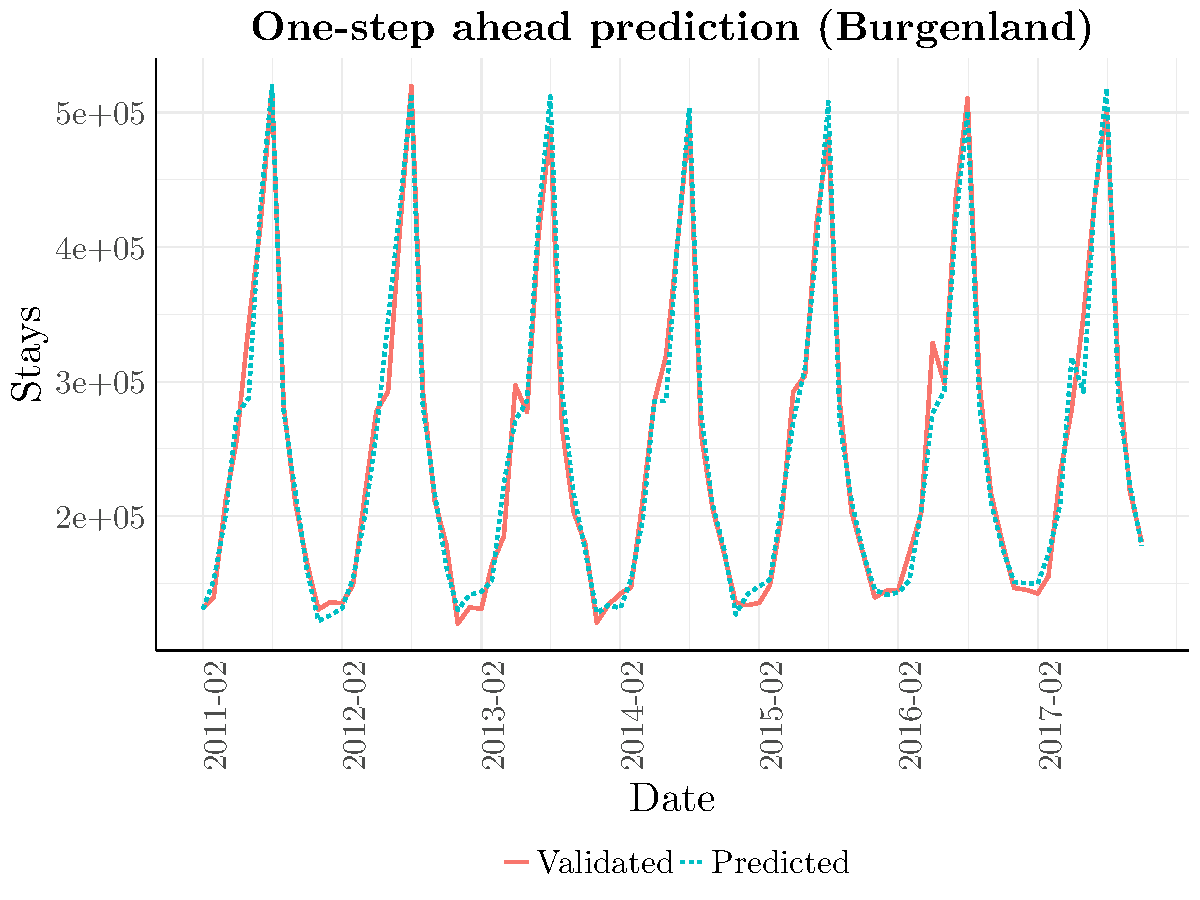
\includegraphics[width=1\textwidth]{images/RFR/Burgenland_one_step_ahead.pdf}
\end{minipage}
\begin{minipage}[h!]{0.33\textwidth}
\centering
    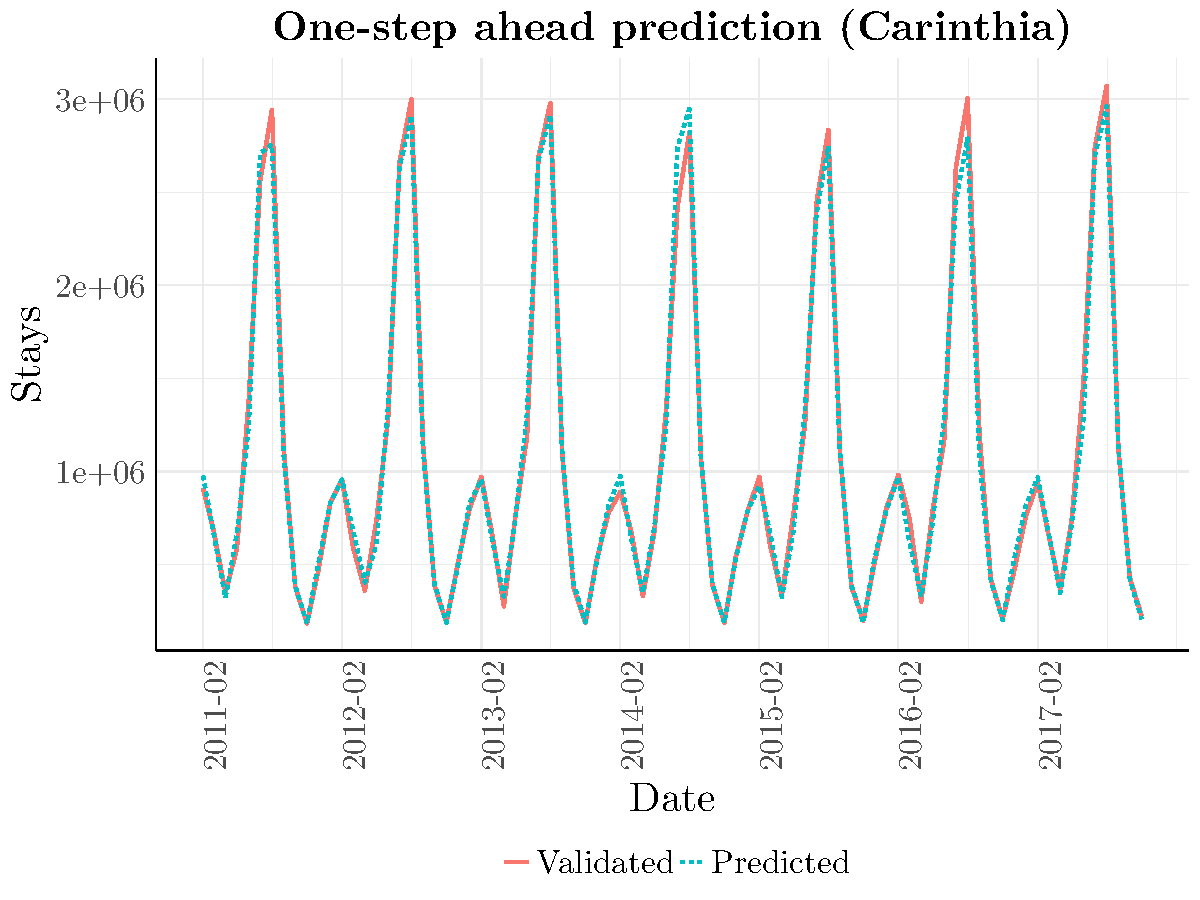
\includegraphics[width=1\textwidth]{images/RFR/Carinthia_one_step_ahead.pdf}
\end{minipage}
\begin{minipage}[h!]{0.33\textwidth}
\centering
    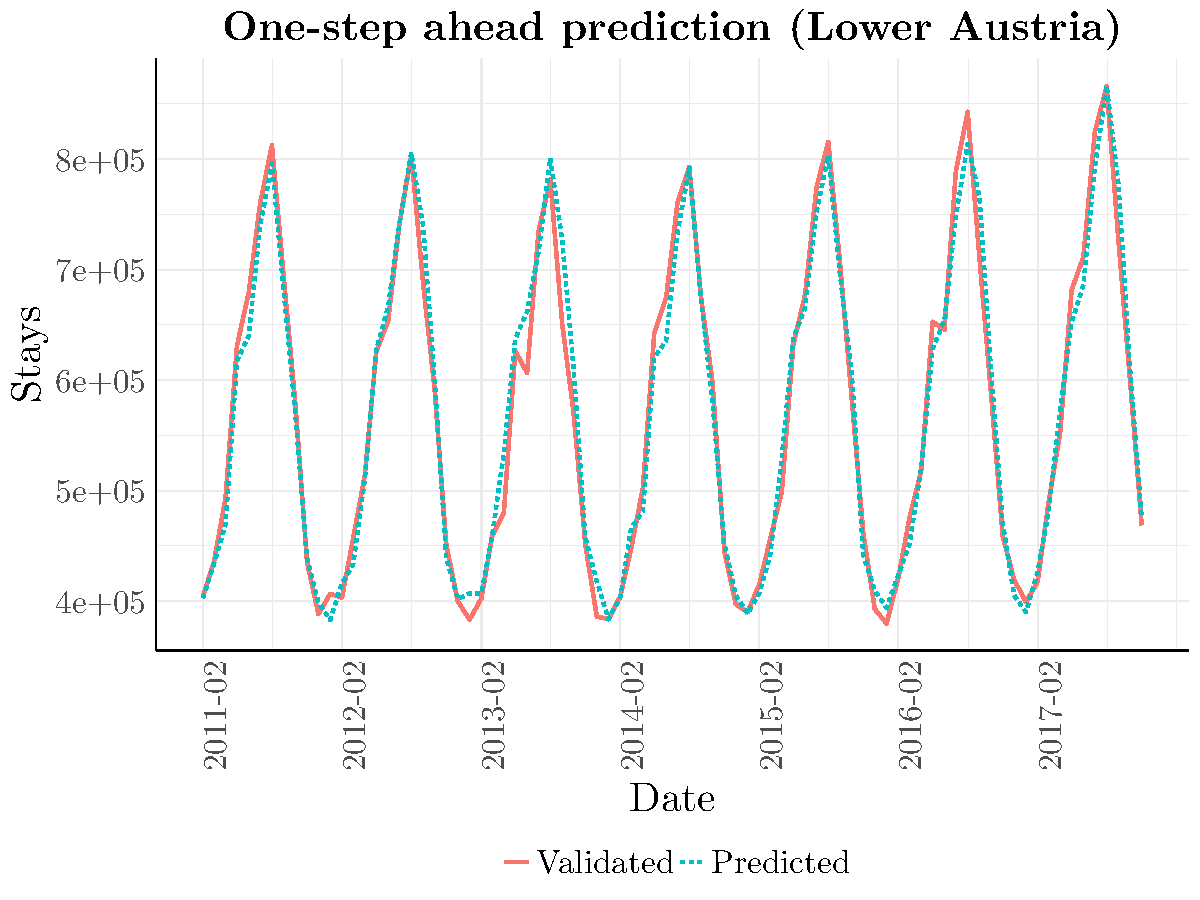
\includegraphics[width=1\textwidth]{images/RFR/Lower_Austria_one_step_ahead.pdf}
\end{minipage}
\begin{minipage}[h!]{0.33\textwidth}
\centering
    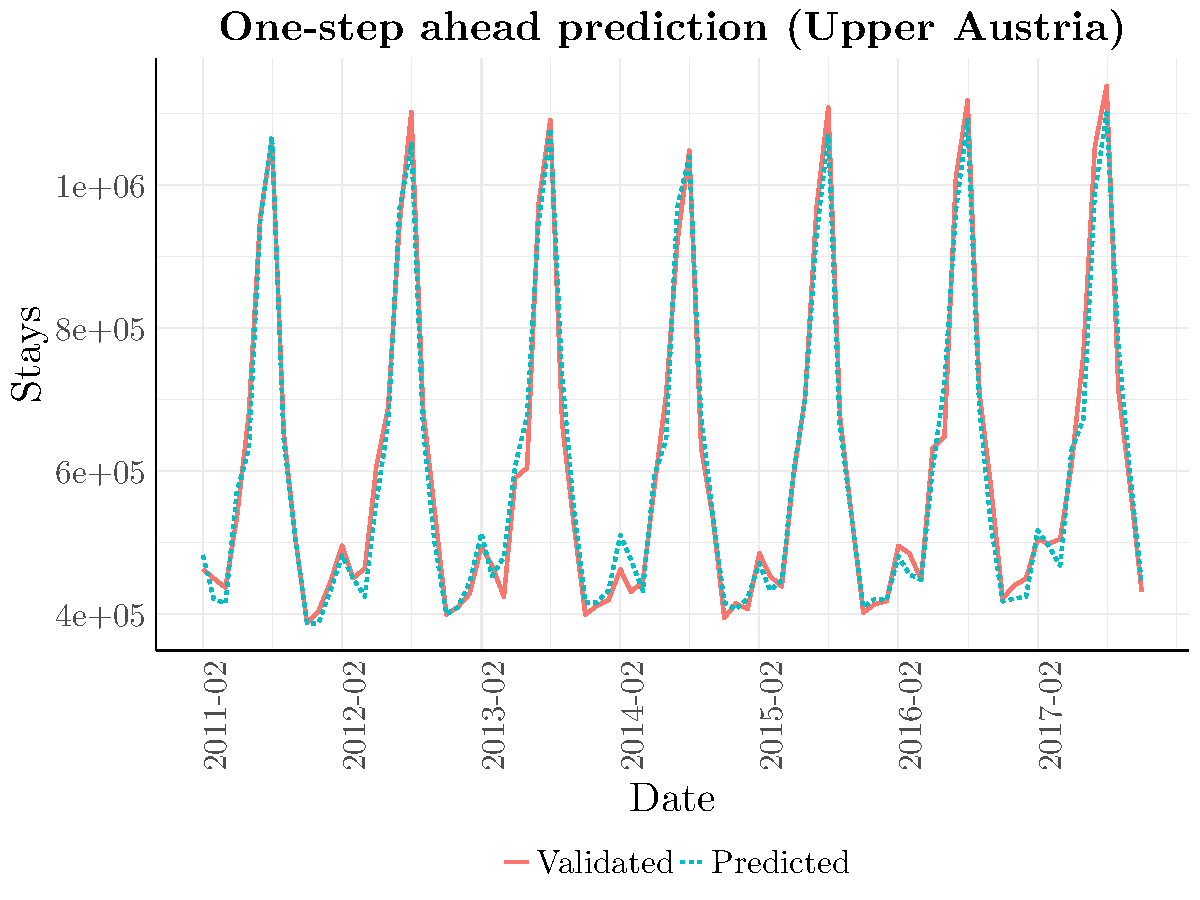
\includegraphics[width=1\textwidth]{images/RFR/Upper_Austria_one_step_ahead.pdf}
\end{minipage}
\begin{minipage}[h!]{0.33\textwidth}
\centering
    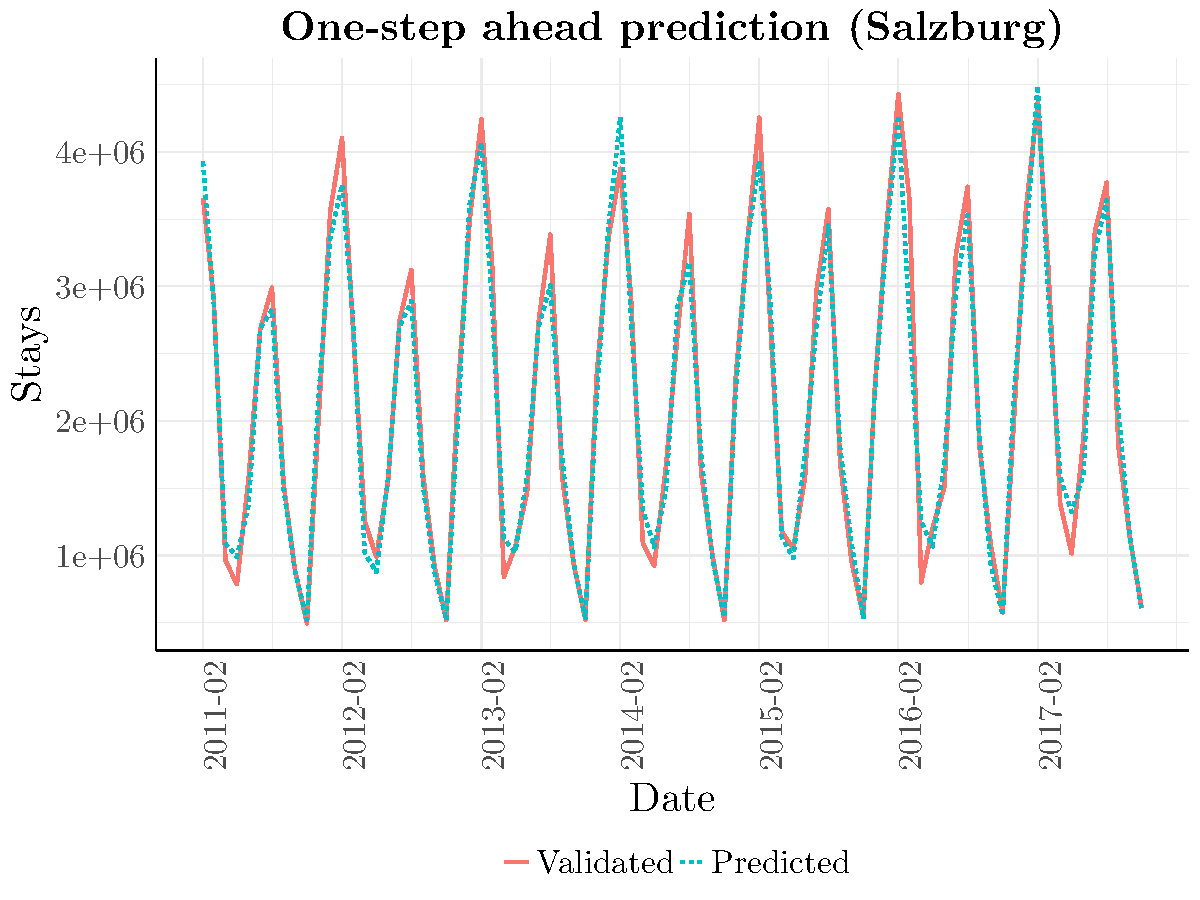
\includegraphics[width=1\textwidth]{images/RFR/Salzburg_one_step_ahead.pdf}
\end{minipage}
\begin{minipage}[h!]{0.33\textwidth}
\centering
    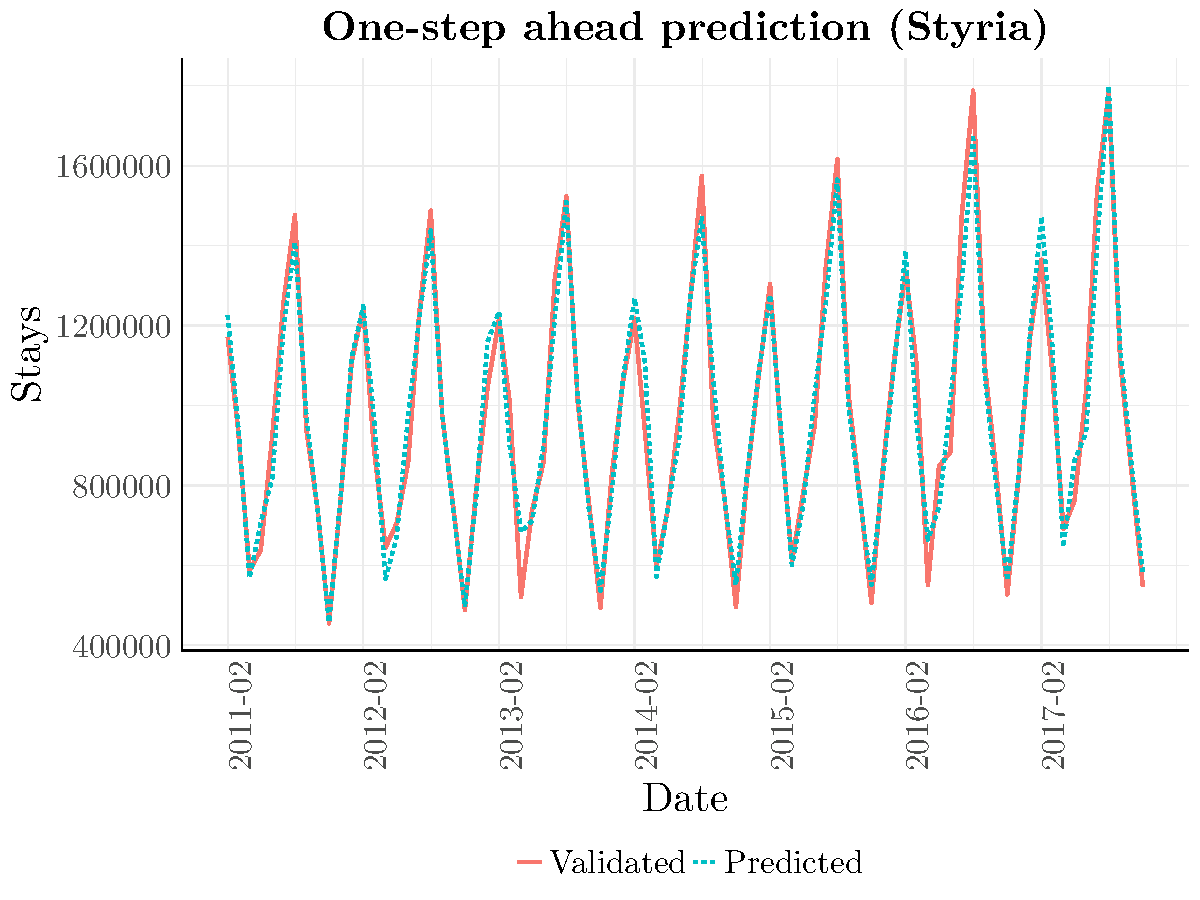
\includegraphics[width=1\textwidth]{images/RFR/Styria_one_step_ahead.pdf}
\end{minipage}
\begin{minipage}[h!]{0.33\textwidth}
\centering
    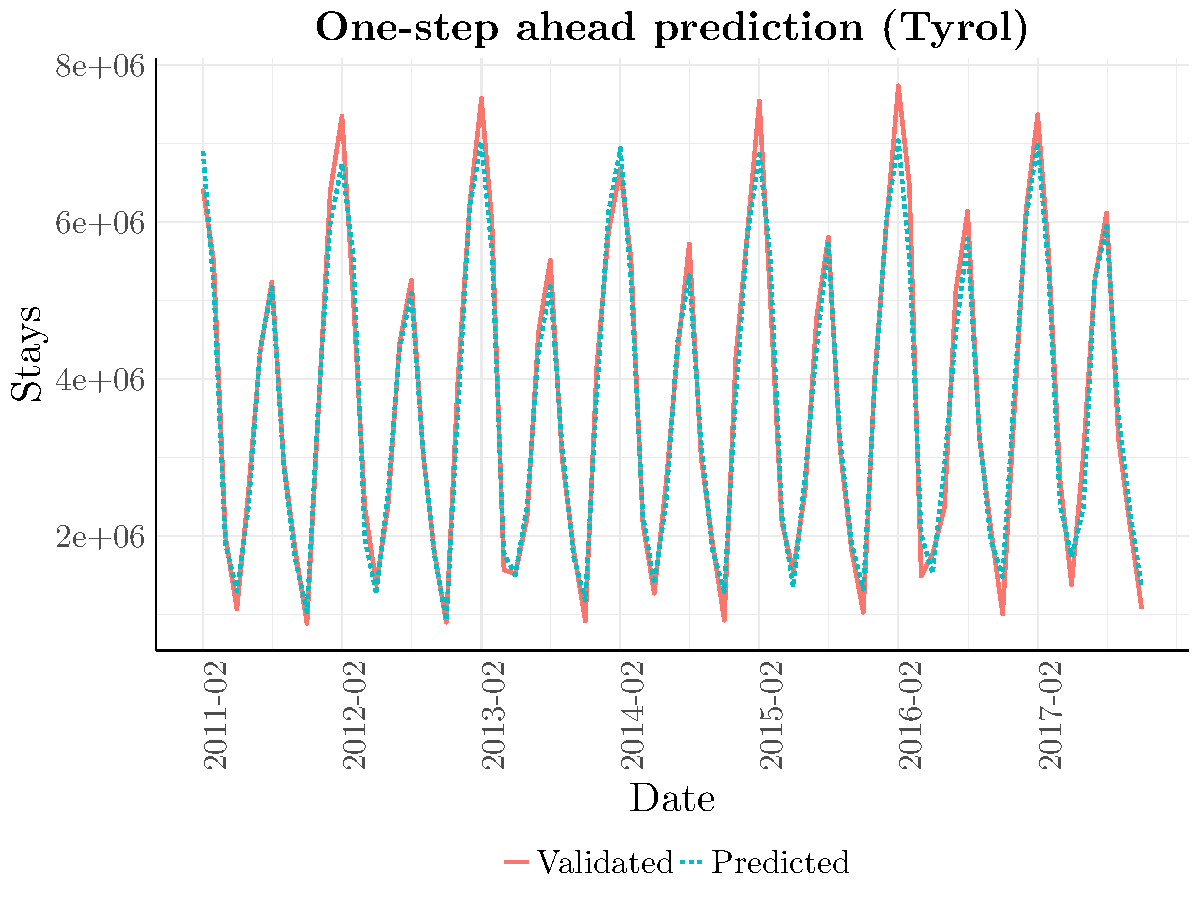
\includegraphics[width=1\textwidth]{images/RFR/Tyrol_one_step_ahead.pdf}
\end{minipage}
\begin{minipage}[h!]{0.33\textwidth}
\centering
    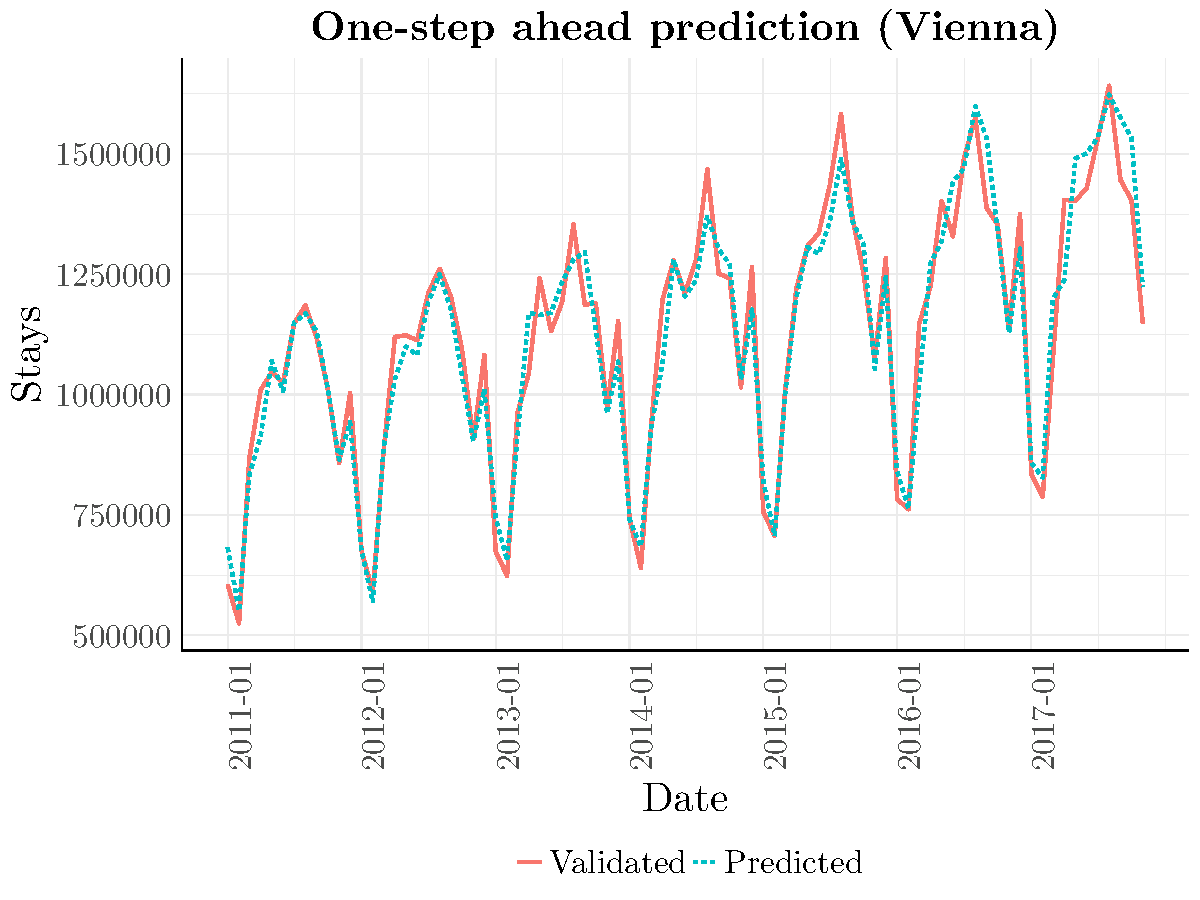
\includegraphics[width=1\textwidth]{images/RFR/Vienna_one_step_ahead.pdf}
\end{minipage}
\begin{minipage}[h!]{0.33\textwidth}
\centering
    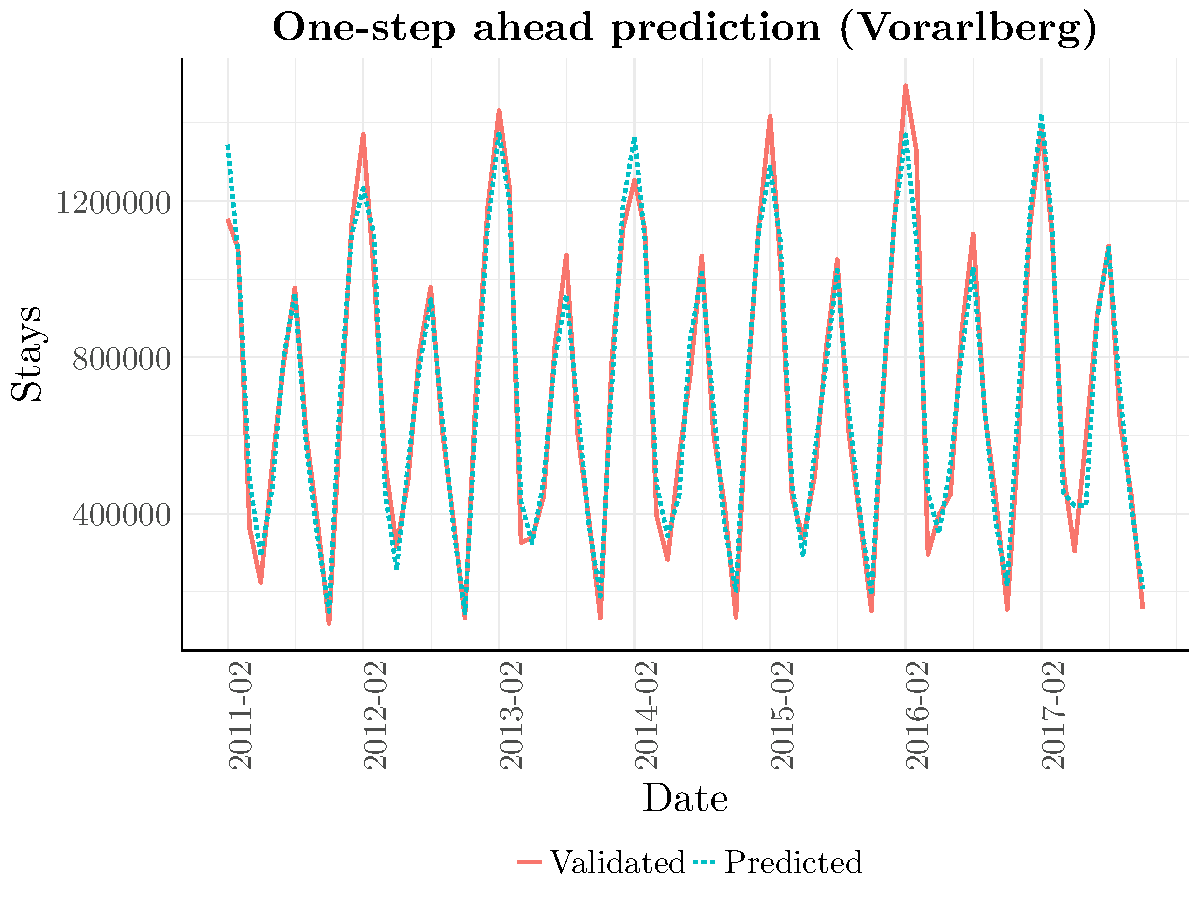
\includegraphics[width=1\textwidth]{images/RFR/Vorarlberg_one_step_ahead.pdf}
\end{minipage}
\caption{Comparison of predicted and validated time series from 01/2011 to 11/2017 (Note the different scaling of the y-axis.).}
\label{fig:rfr_onestep_comp}
\end{figure} 
\newpage
\noindent
In forecasting it is more important to predict over multiple steps rather than one. Therefore, multistep-prediction was implemented for \textit{RFR}. %, which should use predicted data as input for the next prediction. %Since the presented \textit{RFR} model uses lagged time series as predictors, original stays values were replaced such that the current prediction serves as an explanatory value for the forecasting step \textit{"lag-steps ahead"} (i.e. 1, 6, 11, 12-steps ahead). 
%To get a visual impression of what changes when n-step ahead prediction is used, a
A comparison of one-step and n-step ahead prediction for Vienna can been seen in figure \ref{fig:rfr_one_n_step_vienna}. The n-step ahead predicted curve experiences a slight shift of the main peak and a smoother time series with no inter-annual variability. RMSE and R$^2$ of the other provinces are shown in table \ref{tab:n_step}. When using n-step ahead prediction, the RMSE increases (amplitude depending on seasonal complexity) and R$^2$ decreases. %A lack in temporal agreement is also visible in figure \ref{fig:rfr_one_n_step_vienna}. 
\newpage
\begin{longtable}[h!]
{!{\vrule width0.05cm}g!{\vrule width0.05cm}g!{\vrule width0.05cm}g!{\vrule width0.05cm}g!{\vrule width0.05cm}g!{\vrule width0.05cm}g!{\vrule width0.05cm}g!{\vrule width0.05cm}g!{\vrule width0.05cm}g!{\vrule width0.05cm}g!{\vrule width0.05cm}}
\caption{Error metrics resulting when using n-step ahead prediction with the final \textit{RFR} model. Green represents the best province, red the worst.}
\label{tab:n_step}\\
\specialrule{0.05cm}{.0cm}{.0cm}
\multicolumn{1}{!{\vrule width0.05cm}c!{\vrule width0.05cm}}{\bfseries  \par} & \multicolumn{1}{c!{\vrule width0.05cm}}{\bfseries \begin{tabular}[c]{@{}l@{}}Burgen-\\land \end{tabular}\par} & 
\multicolumn{1}{c!{\vrule width0.05cm}}{\bfseries Carinthia \par} & 
\multicolumn{1}{c!{\vrule width0.05cm}}{\bfseries \begin{tabular}[c]{@{}l@{}}Lower \\ Austria \end{tabular} \par} & 
\multicolumn{1}{c!{\vrule width0.05cm}}{\bfseries \begin{tabular}[c]{@{}l@{}}Upper \\ Austria \end{tabular} \par} & \multicolumn{1}{c!{\vrule width0.05cm}}{\bfseries \begin{tabular}[c]{@{}l@{}} Salz-\\burg \end{tabular} \par} & \multicolumn{1}{c!{\vrule width0.05cm}}{\bfseries Styria \par} &
\multicolumn{1}{c!{\vrule width0.05cm}}{\bfseries Tyrol \par} &
\multicolumn{1}{c!{\vrule width0.05cm}}{\bfseries \begin{tabular}[c]{@{}l@{}} Vorarl-\\berg\end{tabular} \par} \\ 
\specialrule{0.05cm}{.0cm}{.0cm} 
{\bfseries RMSE \par} &  \cellcolor[HTML]{66bd63} 19522 &  \cellcolor[HTML]{fee08b} 87145 &  \cellcolor[HTML]{a6d96a} 33597 &  \cellcolor[HTML]{d9ef8b} 36349 &  \cellcolor[HTML]{f46d43} 309324 & \cellcolor[HTML]{fdae61} 110711 & \cellcolor[HTML]{d73027} 431814 &  \cellcolor[HTML]{ffffbf} 77906 \\ \specialrule{0.025cm}{.0cm}{.0cm}
\rowcolor{white}{\bfseries R$^{2}$ \par} & \cellcolor[HTML]{d9ef8b} 0.9774 &  \cellcolor[HTML]{66bd63} 0.9896 & \cellcolor[HTML]{f46d43} 0.9483 & \cellcolor[HTML]{a6d96a} 0.9799 & \cellcolor[HTML]{fdae61} 0.9556 & \cellcolor[HTML]{d73027} 0.8787 &  \cellcolor[HTML]{ffffbf} 0.9652 & \cellcolor[HTML]{fee08b} 0.9614  \\ 
\specialrule{0.05cm}{.0cm}{.0cm}
\end{longtable}
\begin{figure}[h!]
\centering
\begin{minipage}[h!]{0.49\textwidth}
\centering
    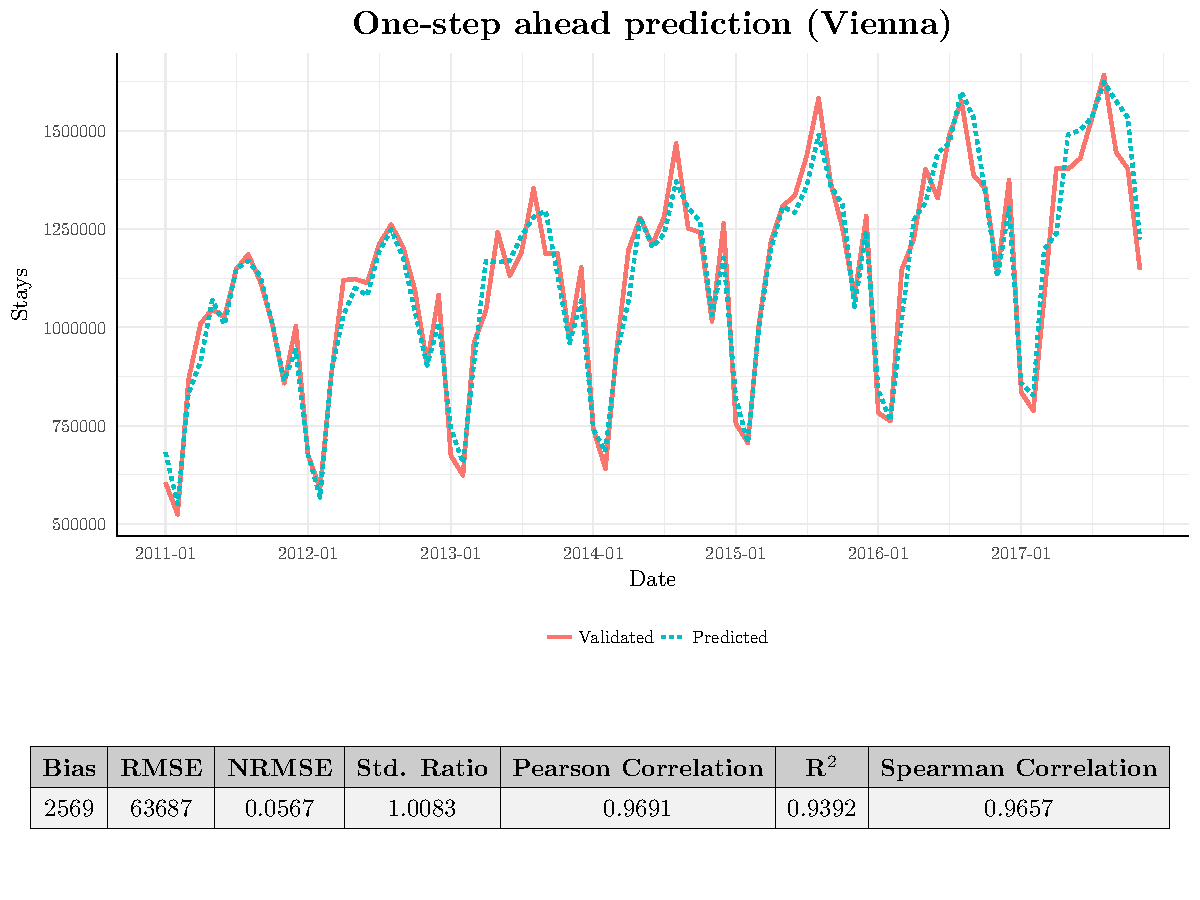
\includegraphics[width=1\textwidth]{images/RFR/Vienna_one_step_ahead_2.pdf}
\end{minipage}
\hspace{0.1cm}
\begin{minipage}[h!]{0.49\textwidth}
\centering
    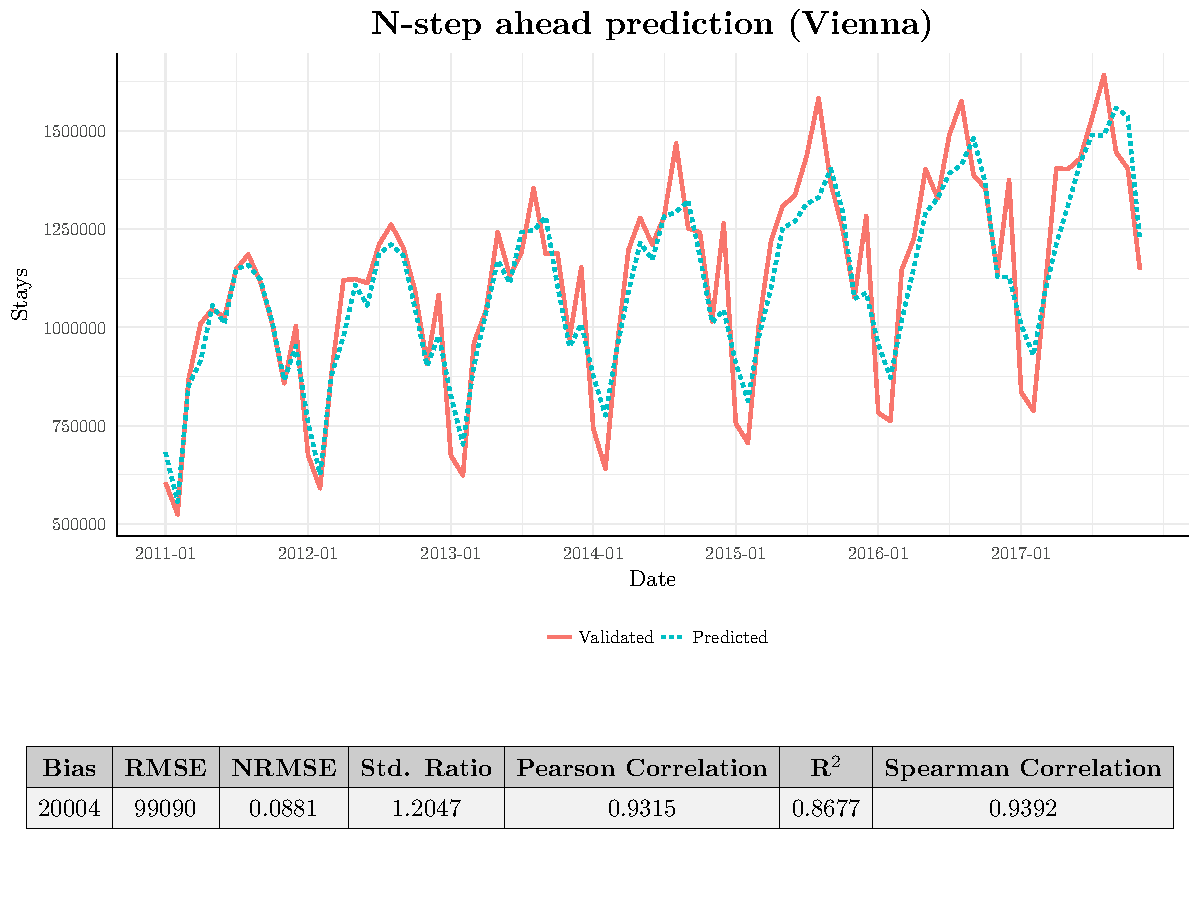
\includegraphics[width=1\textwidth]{images/RFR/Vienna_n_step_ahead.pdf}
\end{minipage}
    \caption{Comparison of one-step (left) and n-step (right) ahead prediction for Vienna.}
	 \label{fig:rfr_one_n_step_vienna}
\end{figure} 
\subsubsection{Summary and Discussion}
\label{sssec:rfr_disc}
\textit{RFR} based on stacked province-wise lagged data has clearly shown to be applicable and leading to satisfying results. Only little success could be achieved by using province-wise training. This is reasonable, since the \textit{RFR} model only knows values, which have occurred in the past.  If there is any trend (values not known/trained), \textit{RFR} is not able to handle it properly. Furthermore, it was found out that \textit{RFR} for provinces comprising a two-seasonal tourist stays pattern performs worst. The complex and rapid changes of stays are difficult to be modelled by \textit{RFR}, since the mean value of many single predictions smooths the predicted curve (section \ref{sssec:meth}). This could be a reasonable explanation for larger deviations in Tirol, Salzburg, Styria and Vorarlberg.   
\\
\\
Having a closer look at table \ref{tab:t_all} and \ref{tab:rfr_final_stats} reveals that better statistics can be obtained by using a province-wise \textit{RFR} model for two-seasonal provinces, whereas for Vienna results improve with the chosen configuration. Including lagged stays data from first-order neighbours did not improve forecasting and made it even worse. A reason could be that neighbouring provinces do not have a clear overlap of the seasonal onset and there are too many predictors (necessary to adjust \texttt{mtry}).   
\\
\\
To sum up, \textit{RFR} is a very simple method to use and observed changes by adjusting the used parameters were really small. %According to previously mentioned papers, it can be approved that it is sufficient enough to just use a large number of trees and an elaborated choice of predictors. 
%Moreover, \textit{"feature bagging"} leads to an improvement of the model, but at an expense of interpretability of the results. 
Predictions with \textit{RFR} could be further improved by including other predictors such as economy data of province-wise income resulting from tourism.
\newpage
\subsection{(ST)ARIMA}
\label{ssec:starima}
\fancyhead[R]{Methods: (ST)ARIMA}
A short decomposition of the acronym \textit{(ST)ARIMA} helps to understand what it includes. The simplest form are the autoregressive (AR) and moving average (MA) model. Combined together, they form the ARMA model which was first described by \cite{gurland1954hypothesis}, but got only popular after the publication of \cite{BoxGeorgeE.P1970TSAF}. The integration part (I) was added to create \textit{ARIMA} for handling non-stationary data, i.e. trends or seasonal data. The spatio-temporal ARIMA (\textit{STARIMA}) model proposed by \cite{pfeifer1981seasonal} is an extension of the \textit{ARIMA} model incorporating spatial autocorrelation. Both, \textit{ARIMA} and \textit{STARIMA} explicitly model a time series' behaviour based on its past values. There is no possiblity to include other explanatory variables. While the ARMA and \textit{ARIMA} model are well established and used for analysing time series throughout all different disciplines, the \textit{STARIMA} model seems to be far less used. \cite{Islam-KhanRezwan2012PTTi, ChengTao2014ADSW, PeiboDuan2016Stpw} use the latter for traffic flow predictions.
\subsubsection{Methodology}
The $ARIMA(p,d,q)$ model combines the following three parts:
\begin{itemize}
\item AR($p$): Auto-regressive term of order $p$. Describes a linear regression of the current value against the p previous values.
\item I($d$): Differentiation of order $d$ (number of differences). Used for achieving stationarity of the time series.
\item MA($q$): Moving average term of order $q$. Describes a linear regression of the current value against the forecast errors of the previous values.
\end{itemize}
\textit{ARIMA} can be extended by a seasonal model as proposed by \cite{pfeifer1981seasonal} accommodating e.g. daily, weekly or annual cycles. The seasonal model is basically a second \textit{ARIMA} model with a different lag used for the differentiation. The model is then extended to $ARIMA(p,d,q)(P,D,Q)_S$, where $P$, $D$ and $Q$ are the equivalents to the lower-case letters and $S$ indicates the lag used for the seasonal model. The parameters are usually estimated using either a brute-force grid search or the Box-Jenkins method (\cite{BoxGeorgeE.P1970TSAF}). The latter uses the ACF to estimate $p$ and PACF to estimate $q$. Furthermore, the ACF is used for the decision whether a series is stationary or not and the resulting choice of $d$. The seasonal model is estimated similarly using the by lag $S$ differentiated data. The \textit{STARIMA} model, the spatio-temporal extension of the \textit{ARIMA}, includes a spatial weight matrix  as input describing to which extent a particular instance should be modelled based on other instances. Often simply neighbourhood first order or a distance related weighting is used.
\\
\\
Unfortunately (ST)ARMA requires (weak) stationary data and spatio-temporal data is often non-stationary, i.e. contains trends and seasonality. Sometimes the (weak) stationarity, i.e. a non-varying mean and auto-covariance over time, can be achieved by a differentiation in the \textit{I} part, thus the use of \textit{(ST)ARIMA}. If not, further pre-processing (e.g. applying the log-function) is necessary.
\subsubsection{Experimental setup}
For the following analysis, R's built-in \textit{ARIMA} function and the \textit{STARIMA} software package for R by Cheng and Wang\footnote{V2.0, January 2012, provided within the course CEGE076 Spatio-Temporal Data Mining} are used. The following differences between the two implementations were noticed and accommodated in an appropriate way:
\begin{itemize}
\item Only the \textit{ARIMA} function allows to apply a seasonal model.
\item \textit{ARIMA} offers a multi-step ahead prediction whereas the \textit{STARIMA} package only offers a one-step ahead prediction
\end{itemize}
Thus, a recursive multi-step ahead prediction for \textit{STARIMA} similar to the one used by \cite{liu2017svm} was implemented by the author, as multi-step ahead prediction seems more appropriate for our experiment.
To handle the seasonality discovered in section \ref{ssec:t_pat}, for \textit{ARIMA} simply a seasonal model with $S=12$ is used while for \textit{STARIMA} the data was differentiated manually by lag 12 in pre-procesing. Compared to fig. \ref{fig:ACFplot} the ACF of the differentiated time series (fig. \ref{fig:STARIMA_ACF_diff12}) show that the seasonality is largely eliminated and now only Vienna show some non-stationary behaviour, which can possibly later be eliminated using the \textit{I} part of the \textit{(ST)ARIMA} model. Additionally, in pre-processing the data was scaled before fitting the models for better numerical performance.
\begin{figure}[h!]
\centering
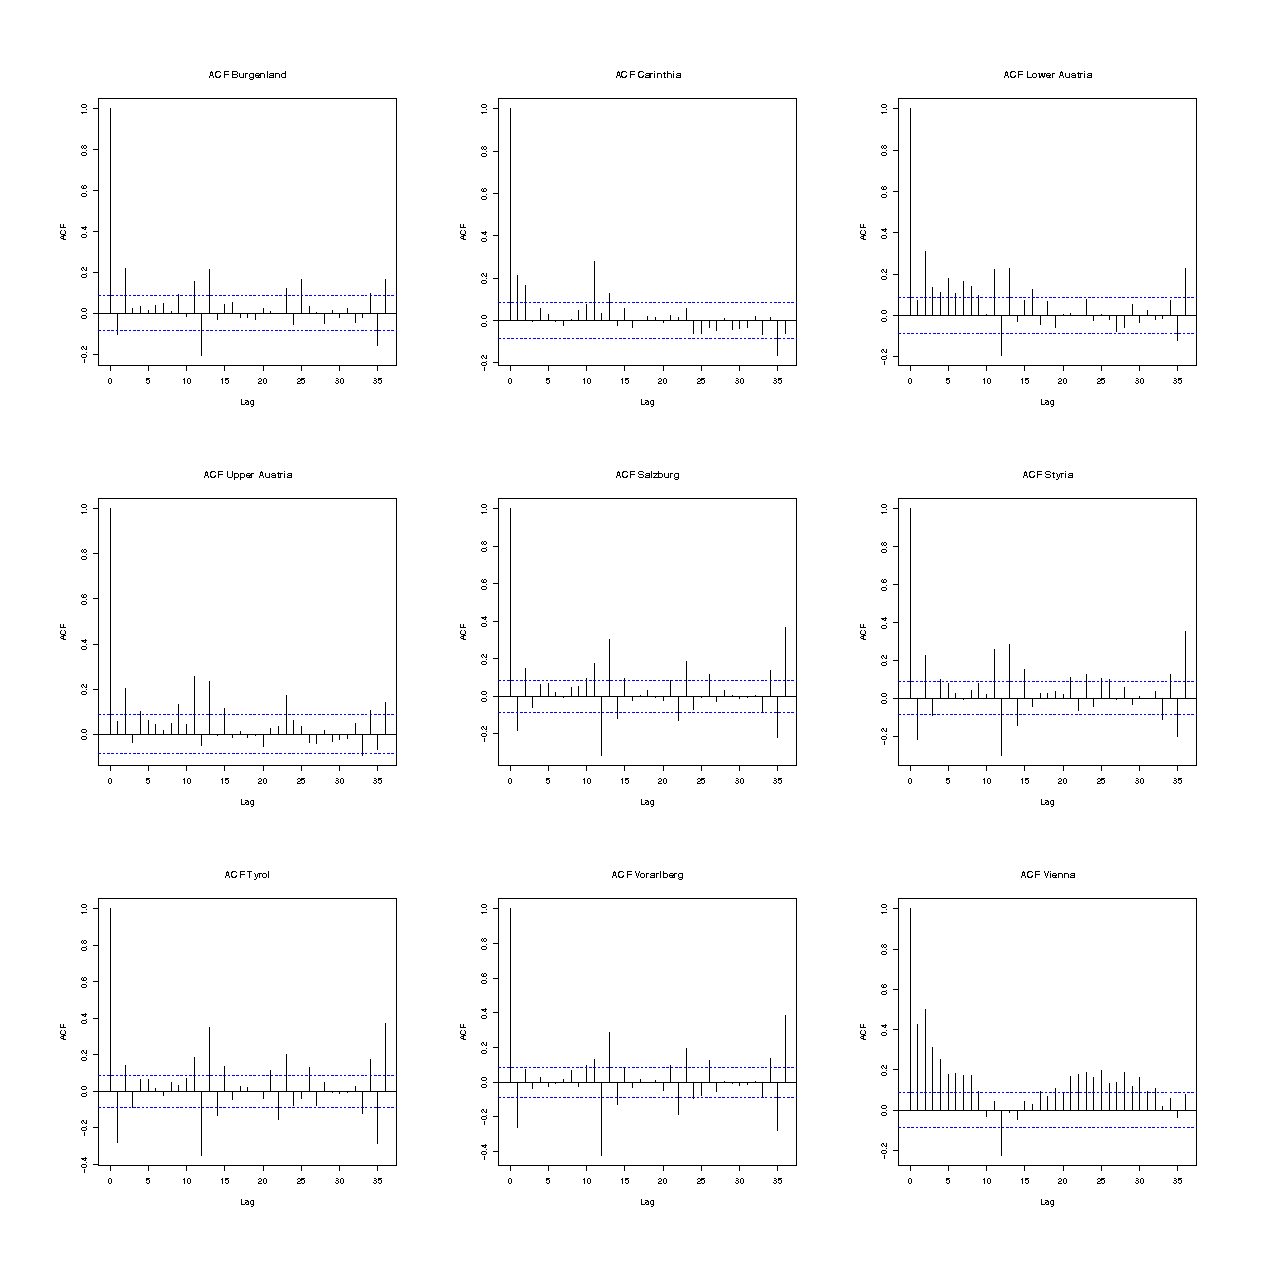
\includegraphics[width=1\textwidth]{images/ARIMA/STARIMA_ACF_stays_diff12.pdf}
\caption{Autocorrelation functions of the time series differentiated by lag 12 (the blue dashed lines show the 95\% confidence intervals)}
\label{fig:STARIMA_ACF_diff12}
\end{figure}
Four different models \textit{ST1}, \textit{STn}, \textit{STns} and \textit{ARn} were trained and tested (see table \ref{tab:STARIMA_exp}). They differ in the base model used, the number of steps predicted ahead and the range of data used for training of the models. The test data was the same for all models.
\newcolumntype{g}{>{\columncolor{Gray}}l}
\begin{longtable}[h!]
{!{\vrule width0.05cm}g!{\vrule width0.05cm}g!{\vrule width0.05cm}g!{\vrule width0.05cm}g!{\vrule width0.05cm}g!{\vrule width0.05cm}g!{\vrule width0.05cm}g!{\vrule width0.05cm}g!{\vrule width0.05cm}}
\caption{Summary of the models' characteristics}
\label{tab:STARIMA_exp}\\
\specialrule{0.05cm}{.0cm}{.0cm}
\multicolumn{1}{!{\vrule width0.05cm}c!{\vrule width0.05cm}}{\bfseries Model ID \par} & \multicolumn{1}{l!{\vrule width0.05cm}}{\bfseries Model name \par} & \multicolumn{1}{l!{\vrule width0.05cm}}{\bfseries Base model \par} & \multicolumn{1}{l!{\vrule width0.05cm}}{\bfseries Prediction mode \par} & \multicolumn{1}{l!{\vrule width0.05cm}}{\bfseries Training data \par}\\ 
\specialrule{0.05cm}{.0cm}{.0cm} 
ST1 & STARIMA 1-step ahead & STARIMA & single-step & 11/1973 - 12/2010\\ \specialrule{0.025cm}{.0cm}{.0cm}
\rowcolor{white}STn & STARIMA n-step ahead & STARIMA & multi-step (recursive) & 11/1973 - 12/2010\\ \specialrule{0.025cm}{.0cm}{.0cm}
STns & STARIMA n-step ahead short & STARIMA & multi-step (recursive) & 01/2000 - 12/2010\\ \specialrule{0.025cm}{.0cm}{.0cm}
\rowcolor{white}ARn & ARIMA n-step ahead & ARIMA & multi-step & 11/1973 - 12/2010\\
\specialrule{0.05cm}{.0cm}{.0cm}
\end{longtable}
\noindent
For \textit{ARIMA} and \textit{STARIMA} the number of parameters to be estimated is six and three, respectively. A grid search with the range [0,1,2,3] for all parameters is used to find for each province the optimal combination leading to the lowest root-mean square error (RMSE) using the test data (see tables \ref{tab:STARIMA_params_ST1}, \ref{tab:STARIMA_params_STn}, \ref{tab:STARIMA_params_STns} and \ref{tab:STARIMA_params_ARn}). The grid search is applicable, as the paramters of a \textit{(ST)ARIMA} model are usually kept low (\cite{brockwell2002introduction}, chap. 6.5). Regardless of whether the models differ in the base model, prediction mode or even the training data, the optimal parameters are different for almost all provinces. As the upper limit 3 appears several times further sensitivity analysis was executed and showed that larger parameters increase the quality of the models only marginally. The \textit{ARn} shows only a seasonal model for Vienna which does not agree with the interpretation of fig. \ref{fig:STARIMA_ACF_diff12}.
\\
\\
\begin{minipage}[h!]{0.49\textwidth}
\centering
\newcolumntype{g}{>{\columncolor{Gray}}l}
\begin{longtable}[h!]
{!{\vrule width0.05cm}g!{\vrule width0.05cm}g!{\vrule width0.05cm}g!{\vrule width0.05cm}g!{\vrule width0.05cm}g!{\vrule width0.05cm}}
\caption{Model \textit{ST1}: Optimal parameters}
\label{tab:STARIMA_params_ST1}\\
\specialrule{0.05cm}{.0cm}{.0cm}
\multicolumn{1}{!{\vrule width0.05cm}c!{\vrule width0.05cm}}{\bfseries Province \par} & \multicolumn{1}{l!{\vrule width0.05cm}}{\bfseries p \par} & \multicolumn{1}{l!{\vrule width0.05cm}}{\bfseries d \par} & \multicolumn{1}{l!{\vrule width0.05cm}}{\bfseries q \par}\\ 
\specialrule{0.05cm}{.0cm}{.0cm} 
Burgenland & 2 & 0 & 1\\ \specialrule{0.025cm}{.0cm}{.0cm}
\rowcolor{white}Carinthia & 2 & 0 & 2\\ \specialrule{0.025cm}{.0cm}{.0cm}
Lower Austria & 2 & 1 & 0\\ \specialrule{0.025cm}{.0cm}{.0cm}
\rowcolor{white}Upper Austria & 3 & 0 & 3\\ \specialrule{0.025cm}{.0cm}{.0cm}
Salzburg & 1 & 0 & 3\\ \specialrule{0.025cm}{.0cm}{.0cm}
\rowcolor{white}Styria & 3 & 0 & 3\\ \specialrule{0.025cm}{.0cm}{.0cm}
Tyrol & 1 & 0 & 2\\ \specialrule{0.025cm}{.0cm}{.0cm}
\rowcolor{white}Vorarlberg & 1 & 0 & 1\\ \specialrule{0.025cm}{.0cm}{.0cm}
Vienna & 2 & 1 & 3\\ \specialrule{0.05cm}{.0cm}{.0cm}
\end{longtable}
\end{minipage}
\begin{minipage}[h!]{0.49\textwidth}
\centering
\newcolumntype{g}{>{\columncolor{Gray}}l}
\begin{longtable}[h!]
{!{\vrule width0.05cm}g!{\vrule width0.05cm}g!{\vrule width0.05cm}g!{\vrule width0.05cm}g!{\vrule width0.05cm}g!{\vrule width0.05cm}}
\caption{Model \textit{STn}: Optimal parameters}
\label{tab:STARIMA_params_STn}\\
\specialrule{0.05cm}{.0cm}{.0cm}
\multicolumn{1}{!{\vrule width0.05cm}c!{\vrule width0.05cm}}{\bfseries Province \par} & \multicolumn{1}{l!{\vrule width0.05cm}}{\bfseries p \par} & \multicolumn{1}{l!{\vrule width0.05cm}}{\bfseries d \par} & \multicolumn{1}{l!{\vrule width0.05cm}}{\bfseries q \par}\\ 
\specialrule{0.05cm}{.0cm}{.0cm} 
Burgenland & 2 & 1 & 0\\ \specialrule{0.025cm}{.0cm}{.0cm}
\rowcolor{white}Carinthia & 2 & 0 & 0\\ \specialrule{0.025cm}{.0cm}{.0cm}
Lower Austria & 3 & 1 & 2\\ \specialrule{0.025cm}{.0cm}{.0cm}
\rowcolor{white}Upper Austria & 2 & 1 & 0\\ \specialrule{0.025cm}{.0cm}{.0cm}
Salzburg & 1 & 0 & 1\\ \specialrule{0.025cm}{.0cm}{.0cm}
\rowcolor{white}Styria & 2 & 1 & 3\\ \specialrule{0.025cm}{.0cm}{.0cm}
Tyrol & 3 & 0 & 2\\ \specialrule{0.025cm}{.0cm}{.0cm}
\rowcolor{white}Vorarlberg & 3 & 1 & 3\\ \specialrule{0.025cm}{.0cm}{.0cm}
Vienna & 2 & 1 & 2\\ \specialrule{0.05cm}{.0cm}{.0cm}
\end{longtable}
\end{minipage}
\clearpage
\newpage
\hspace{-0.7cm}
\begin{minipage}[h!]{0.49\textwidth}
\centering
\newcolumntype{g}{>{\columncolor{Gray}}l}
\begin{longtable}[h!]
{!{\vrule width0.05cm}g!{\vrule width0.05cm}g!{\vrule width0.05cm}g!{\vrule width0.05cm}g!{\vrule width0.05cm}g!{\vrule width0.05cm}}
\caption{Model \textit{STns}: Optimal parameters}
\label{tab:STARIMA_params_STns}\\
\specialrule{0.05cm}{.0cm}{.0cm}
\multicolumn{1}{!{\vrule width0.05cm}c!{\vrule width0.05cm}}{\bfseries Province \par} & \multicolumn{1}{l!{\vrule width0.05cm}}{\bfseries p \par} & \multicolumn{1}{l!{\vrule width0.05cm}}{\bfseries d \par} & \multicolumn{1}{l!{\vrule width0.05cm}}{\bfseries q \par}\\ 
\specialrule{0.05cm}{.0cm}{.0cm} 
Burgenland & 2 & 1 & 0\\ \specialrule{0.025cm}{.0cm}{.0cm}
\rowcolor{white}Carinthia & 2 & 0 & 2\\ \specialrule{0.025cm}{.0cm}{.0cm}
Lower Austria & 3 & 1 & 3\\ \specialrule{0.025cm}{.0cm}{.0cm}
\rowcolor{white}Upper Austria & 3 & 1 & 1\\ \specialrule{0.025cm}{.0cm}{.0cm}
Salzburg & 3 & 1 & 1\\ \specialrule{0.025cm}{.0cm}{.0cm}
\rowcolor{white}Styria & 1 & 1 & 2\\ \specialrule{0.025cm}{.0cm}{.0cm}
Tyrol & 3 & 1 & 1\\ \specialrule{0.025cm}{.0cm}{.0cm}
\rowcolor{white}Vorarlberg & 2 & 1 & 3\\ \specialrule{0.025cm}{.0cm}{.0cm}
Vienna & 2 & 1 & 0\\ \specialrule{0.05cm}{.0cm}{.0cm}
\end{longtable}
\end{minipage}
\begin{minipage}[h!]{0.49\textwidth}
\centering
\newcolumntype{g}{>{\columncolor{Gray}}l}
\begin{longtable}[h!]
{!{\vrule width0.05cm}g!{\vrule width0.05cm}g!{\vrule width0.05cm}g!{\vrule width0.05cm}g!{\vrule width0.05cm}g!{\vrule width0.05cm}g!{\vrule width0.05cm}g!{\vrule width0.05cm}g!{\vrule width0.05cm}}
\caption{Model \textit{ARn}: Optimal parameters; the seasonal model is of order $S=12$}
\label{tab:STARIMA_params_ARn}\\
\specialrule{0.05cm}{.0cm}{.0cm}
\multicolumn{1}{!{\vrule width0.05cm}c!{\vrule width0.05cm}}{\bfseries Province \par} & \multicolumn{1}{l!{\vrule width0.05cm}}{\bfseries p \par} & \multicolumn{1}{l!{\vrule width0.05cm}}{\bfseries d \par} & \multicolumn{1}{l!{\vrule width0.05cm}}{\bfseries q \par} & \multicolumn{1}{l!{\vrule width0.05cm}}{\bfseries P \par} & \multicolumn{1}{l!{\vrule width0.05cm}}{\bfseries D \par} & \multicolumn{1}{l!{\vrule width0.05cm}}{\bfseries Q \par}\\ 
\specialrule{0.05cm}{.0cm}{.0cm} 
Burgenland & 3 & 0 & 2 & 2 & 0 & 1\\ \specialrule{0.025cm}{.0cm}{.0cm}
\rowcolor{white}Carinthia & 3 & 0 & 0 & 3 & 1 & 2\\ \specialrule{0.025cm}{.0cm}{.0cm}
Lower Austria & 3 & 2 & 1 & 0 & 1 & 1\\ \specialrule{0.025cm}{.0cm}{.0cm}
\rowcolor{white}Upper Austria & 3 & 2 & 2 & 0 & 1 & 1\\ \specialrule{0.025cm}{.0cm}{.0cm}
Salzburg & 1 & 2 & 3 & 3 & 1 & 3\\ \specialrule{0.025cm}{.0cm}{.0cm}
\rowcolor{white}Styria & 2 & 2 & 3 & 0 & 1 & 3\\ \specialrule{0.052cm}{.0cm}{.0cm}
Tyrol & 0 & 1 & 3 & 0 & 1 & 0\\ \specialrule{0.025cm}{.0cm}{.0cm}
\rowcolor{white}Vorarlberg & 0 & 2 & 0 & 3 & 1 & 3\\ \specialrule{0.025cm}{.0cm}{.0cm}
Vienna & 0 & 0 & 0 & 2 & 1 & 2\\ \specialrule{0.05cm}{.0cm}{.0cm}
\end{longtable}
\end{minipage}
\subsubsection{Results}
As performance measures the RMSE, the normalised RMSE (NRMSE) and the R$^2$ were used. While (N)RMSE measures the errors between the prediction and the observed data, R$^2$ is a measure for the similarity of the shape. As tables \ref{tab:STARIMA_perf_ST1}, \ref{tab:STARIMA_perf_STn}, \ref{tab:STARIMA_perf_STns} and \ref{tab:STARIMA_perf_ARn} show, all four models performed reasonably well. The best performing model for each province and each measure are listed in table \ref{tab:STARIMA_perf_overview}. Although there is no dominant model, model \textit{ARn} appears most often. The only experiment that never performs best is the \textit{STn}. The predicted values of the most often best performing \textit{ARn} model show generally a good agreement with the observed data (fig. \ref{fig:STARIMA_ARn_overview}).
\begin{minipage}[h!]{0.49\textwidth}
\centering
\newcolumntype{g}{>{\columncolor{Gray}}l}
\newcolumntype{h}{>{\columncolor{Gray}}r}
\begin{longtable}[h!]
{!{\vrule width0.05cm}g!{\vrule width0.05cm}h!{\vrule width0.05cm}h!{\vrule width0.05cm}h!{\vrule width0.05cm}}
\caption{Model \textit{ST1}: Performance measures}
\label{tab:STARIMA_perf_ST1}\\
\specialrule{0.05cm}{.0cm}{.0cm}
\multicolumn{1}{!{\vrule width0.05cm}c!{\vrule width0.05cm}}{\bfseries Province \par} & \multicolumn{1}{l!{\vrule width0.05cm}}{\bfseries RMSE \par} & \multicolumn{1}{l!{\vrule width0.05cm}}{\bfseries NRMSE \par} & \multicolumn{1}{l!{\vrule width0.05cm}}{\bfseries R$^{2}$  \par}\\ 
\specialrule{0.05cm}{.0cm}{.0cm} 
Burgenland & 16,226 & 0.0654 & 0.9806\\ \specialrule{0.025cm}{.0cm}{.0cm}
\rowcolor{white}Carinthia & 81,993 & 0.0781 & 0.9906\\ \specialrule{0.025cm}{.0cm}{.0cm}
Lower Austria & 19,184 & 0.0338 & 0.9825\\ \specialrule{0.025cm}{.0cm}{.0cm}
\rowcolor{white}Upper Austria & 32,772 & 0.0543 & 0.9789\\ \specialrule{0.025cm}{.0cm}{.0cm}
Salzburg & 201,168 & 0.0927 & 0.9721\\ \specialrule{0.025cm}{.0cm}{.0cm}
\rowcolor{white}Styria & 57,091 & 0.0585 & 0.9727\\ \specialrule{0.025cm}{.0cm}{.0cm}
Tyrol & 381,760 & 0.1013 & 0.9653\\ \specialrule{0.025cm}{.0cm}{.0cm}
\rowcolor{white}Vorarlberg & 86,642 & 0.1211 & 0.9481\\ \specialrule{0.025cm}{.0cm}{.0cm}
Vienna & 52,210 & 0.0464 & 0.9588\\ \specialrule{0.05cm}{.0cm}{.0cm}
\end{longtable}
\end{minipage}
\begin{minipage}[h!]{0.49\textwidth}
\centering
\newcolumntype{g}{>{\columncolor{Gray}}l}
\newcolumntype{h}{>{\columncolor{Gray}}r}
\begin{longtable}[h!]
{!{\vrule width0.05cm}g!{\vrule width0.05cm}h!{\vrule width0.05cm}h!{\vrule width0.05cm}h!{\vrule width0.05cm}}
\caption{Model \textit{STn}: Performance measures}
\label{tab:STARIMA_perf_STn}\\
\specialrule{0.05cm}{.0cm}{.0cm}
\multicolumn{1}{!{\vrule width0.05cm}c!{\vrule width0.05cm}}{\bfseries Province \par} & \multicolumn{1}{l!{\vrule width0.05cm}}{\bfseries RMSE \par} & \multicolumn{1}{l!{\vrule width0.05cm}}{\bfseries NRMSE \par} & \multicolumn{1}{l!{\vrule width0.05cm}}{\bfseries R$^{2}$  \par}\\ 
\specialrule{0.05cm}{.0cm}{.0cm} 
Burgenland&16,598&0.0669&0.9823\\ \specialrule{0.025cm}{.0cm}{.0cm}
\rowcolor{white}Carinthia&93,968&0.0895&0.9881\\ \specialrule{0.025cm}{.0cm}{.0cm}
Lower Austria&18,275&0.0322&0.9847\\ \specialrule{0.025cm}{.0cm}{.0cm}
\rowcolor{white}Upper Austria&31,678&0.0525&0.9848\\ \specialrule{0.025cm}{.0cm}{.0cm}
Salzburg&300,198&0.1383&0.9620\\ \specialrule{0.025cm}{.0cm}{.0cm}
\rowcolor{white}Styria&67,985&0.0697&0.9657\\ \specialrule{0.025cm}{.0cm}{.0cm}
Tyrol&387,000&0.1027&0.9743\\ \specialrule{0.025cm}{.0cm}{.0cm}
\rowcolor{white}Vorarlberg&78,188&0.1093&0.9599\\ \specialrule{0.025cm}{.0cm}{.0cm}
Vienna&72,748&0.0647&0.9369\\ \specialrule{0.05cm}{.0cm}{.0cm}
\end{longtable}
\end{minipage}
\\
\begin{minipage}[h!]{0.49\textwidth}
\centering
\newcolumntype{g}{>{\columncolor{Gray}}l}
\newcolumntype{h}{>{\columncolor{Gray}}r}
\begin{longtable}[h!]
{!{\vrule width0.05cm}g!{\vrule width0.05cm}h!{\vrule width0.05cm}h!{\vrule width0.05cm}h!{\vrule width0.05cm}}
\caption{Model \textit{STns}: Performance measures}
\label{tab:STARIMA_perf_STns}\\
\specialrule{0.05cm}{.0cm}{.0cm}
\multicolumn{1}{!{\vrule width0.05cm}c!{\vrule width0.05cm}}{\bfseries Province \par} & \multicolumn{1}{l!{\vrule width0.05cm}}{\bfseries RMSE \par} & \multicolumn{1}{l!{\vrule width0.05cm}}{\bfseries NRMSE \par} & \multicolumn{1}{l!{\vrule width0.05cm}}{\bfseries R$^{2}$  \par}\\ 
\specialrule{0.05cm}{.0cm}{.0cm} 
Burgenland & 16,627 & 0.0670 & 0.9828\\ \specialrule{0.025cm}{.0cm}{.0cm}
\rowcolor{white}Carinthia & 94,894 & 0.0904 & 0.9878\\ \specialrule{0.025cm}{.0cm}{.0cm}
Lower Austria & 18,193 & 0.0320 & 0.9849\\ \specialrule{0.025cm}{.0cm}{.0cm}
\rowcolor{white}Upper Austria & 29,099 & 0.0482 & 0.9869\\ \specialrule{0.025cm}{.0cm}{.0cm}
Salzburg & 296,607 & 0.1366 & 0.9630\\ \specialrule{0.025cm}{.0cm}{.0cm}
\rowcolor{white}Styria & 67,608 & 0.0693 & 0.9662\\ \specialrule{0.025cm}{.0cm}{.0cm}
Tyrol & 367,167 & 0.0974 & 0.9742\\ \specialrule{0.025cm}{.0cm}{.0cm}
\rowcolor{white}Vorarlberg & 75,247 & 0.1052 & 0.9632\\ \specialrule{0.025cm}{.0cm}{.0cm}
Vienna & 73,869 & 0.0657 & 0.9393\\ \specialrule{0.05cm}{.0cm}{.0cm}
\end{longtable}
\end{minipage}
\begin{minipage}[h!]{0.49\textwidth}
\centering
\newcolumntype{g}{>{\columncolor{Gray}}l}
\newcolumntype{h}{>{\columncolor{Gray}}r}
\begin{longtable}[h!]
{!{\vrule width0.05cm}g!{\vrule width0.05cm}h!{\vrule width0.05cm}h!{\vrule width0.05cm}h!{\vrule width0.05cm}}
\caption{Model \textit{ARn}: Performance measures}
\label{tab:STARIMA_perf_ARn}\\
\specialrule{0.05cm}{.0cm}{.0cm}
\multicolumn{1}{!{\vrule width0.05cm}c!{\vrule width0.05cm}}{\bfseries Province \par} & \multicolumn{1}{l!{\vrule width0.05cm}}{\bfseries RMSE \par} & \multicolumn{1}{l!{\vrule width0.05cm}}{\bfseries NRMSE \par} & \multicolumn{1}{l!{\vrule width0.05cm}}{\bfseries R$^{2}$  \par}\\ 
\specialrule{0.05cm}{.0cm}{.0cm} 
Burgenland & 14,539 & 0.0586 & 0.9840\\ \specialrule{0.025cm}{.0cm}{.0cm}
\rowcolor{white}Carinthia & 86,123 & 0.0821 & 0.9901\\ \specialrule{0.025cm}{.0cm}{.0cm}
Lower Austria & 18,025 & 0.0317 & 0.9850\\ \specialrule{0.025cm}{.0cm}{.0cm}
\rowcolor{white}Upper Austria & 28,269 & 0.0468 & 0.9852\\ \specialrule{0.025cm}{.0cm}{.0cm}
Salzburg & 213,680 & 0.0984 & 0.9747\\ \specialrule{0.025cm}{.0cm}{.0cm}
\rowcolor{white}Styria & 68,917 & 0.0707 & 0.9599\\ \specialrule{0.025cm}{.0cm}{.0cm}
Tyrol & 326,693 & 0.0867 & 0.9767\\ \specialrule{0.025cm}{.0cm}{.0cm}
\rowcolor{white}Vorarlberg & 62,134 & 0.0868 & 0.9744\\ \specialrule{0.025cm}{.0cm}{.0cm}
Vienna & 59,897 & 0.0533 & 0.9545\\ \specialrule{0.05cm}{.0cm}{.0cm}
\end{longtable}
\end{minipage}
\newcolumntype{g}{>{\columncolor{Gray}}l}
\begin{longtable}[h!]
{!{\vrule width0.05cm}g!{\vrule width0.05cm}g!{\vrule width0.05cm}g!{\vrule width0.05cm}g!{\vrule width0.05cm}}
\caption{Best performing models according to (N)RMSE and R$^2$, respectively}
\label{tab:STARIMA_perf_overview}\\
\specialrule{0.05cm}{.0cm}{.0cm}
\multicolumn{1}{!{\vrule width0.05cm}c!{\vrule width0.05cm}}{\bfseries Province \par} & \multicolumn{1}{l!{\vrule width0.05cm}}{\bfseries (N)RMSE \par} & \multicolumn{1}{l!{\vrule width0.05cm}}{\bfseries R$^{2}$  \par}\\ 
\specialrule{0.05cm}{.0cm}{.0cm} 
Burgenland & ARn & ARn\\ \specialrule{0.025cm}{.0cm}{.0cm}
\rowcolor{white}Carinthia & ST1 & ST1\\ \specialrule{0.025cm}{.0cm}{.0cm}
Lower Austria & ARn & ARn\\ \specialrule{0.025cm}{.0cm}{.0cm}
\rowcolor{white}Upper Austria & ARn & STns\\ \specialrule{0.025cm}{.0cm}{.0cm}
Salzburg & ST1 & ARn\\ \specialrule{0.025cm}{.0cm}{.0cm}
\rowcolor{white}Styria & ST1 & ST1\\ \specialrule{0.025cm}{.0cm}{.0cm}
Tyrol & ARn & ARn\\ \specialrule{0.025cm}{.0cm}{.0cm}
\rowcolor{white}Vorarlberg & ARn & ARn\\ \specialrule{0.025cm}{.0cm}{.0cm}
Vienna & ST1 & ST1\\ \specialrule{0.05cm}{.0cm}{.0cm}
\end{longtable}
\noindent
\\
\\
\begin{figure}[h!]
\centering
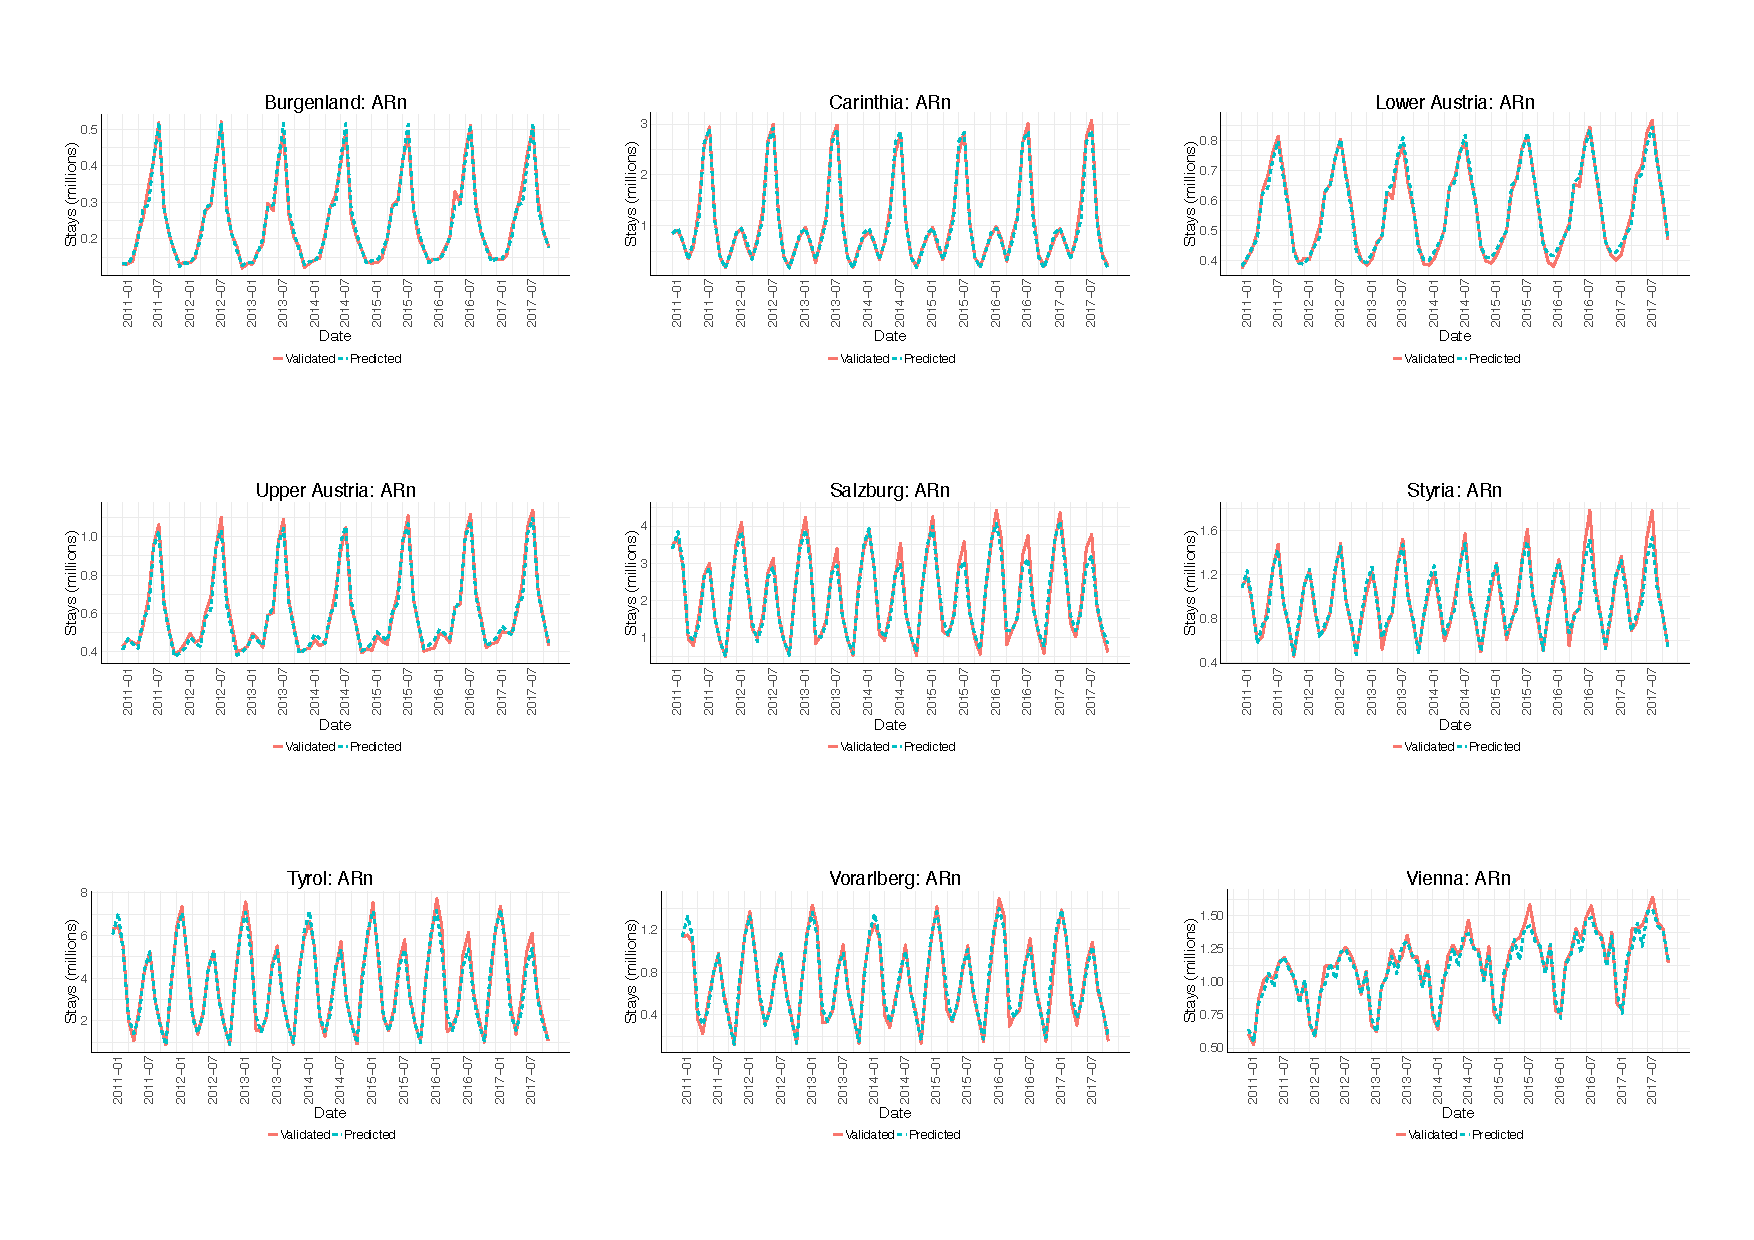
\includegraphics[width=1\textwidth]{images/ARIMA/STARIMA_ARn_overview.pdf}
\caption{Results of the most often best performing \textit{ARn} model}
\label{fig:STARIMA_ARn_overview}
\end{figure}
\newpage
\noindent
The differences of the models can be exemplarily illustrated using the Vienna (fig. \ref{fig:STARIMA_Vienna}). The one-step ahead prediction \textit{ST1} follows the shape of the validated data quite close, especially also in the years 2016 and 2017, resulting in a low (N)RMSE and a high R$^2$ value. \textit{STn} and \textit{STns} look quite similar with minor differences in the prediction for summer 2017. \textit{ARn} can model more accurately the high/low peaks than \textit{STn} and \textit{STns}, i.e. seems to have less smoothing, resulting in a lower RMSE.
\begin{figure}[H]
\centering
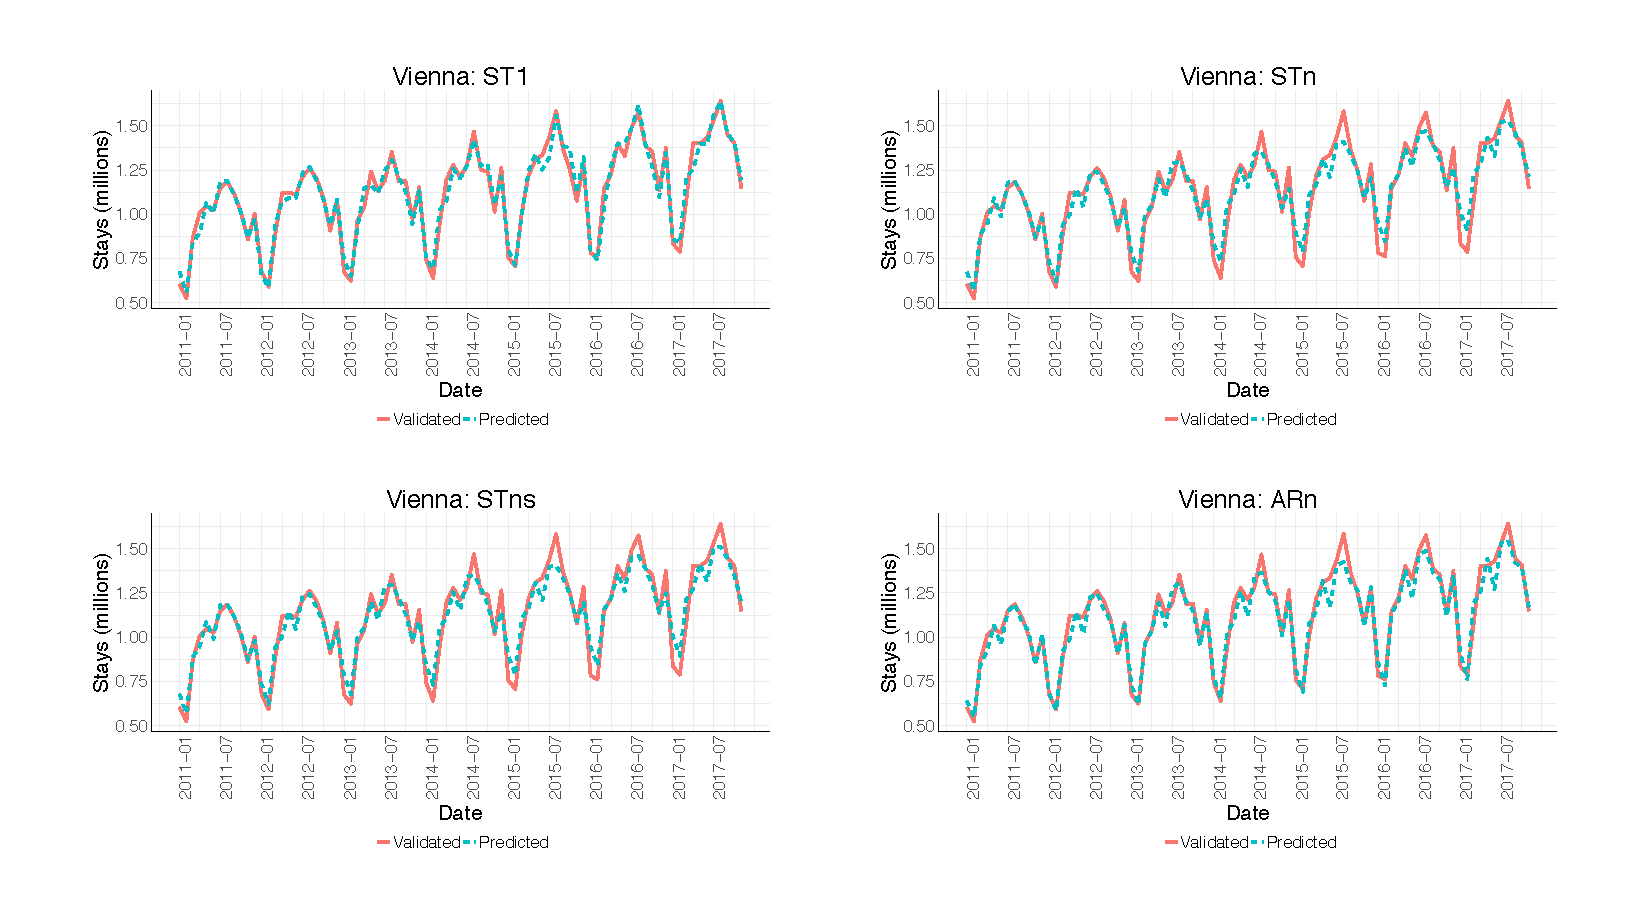
\includegraphics[width=1\textwidth]{images/ARIMA/STARIMA_Vienna.pdf}
\caption{Comparison of the four methods at the example of Vienna}
\label{fig:STARIMA_Vienna}
\end{figure}
\subsubsection{Discussion}
The largest NRMSE values can be found in provinces with two peaks a year which do not evolve similarly over time (e.g. Tyrol, where the winter tourism got more important than the summer tourism in the 1990s). The lowest R$^2$ values has clearly Vienna which has the most complex shape of the time series and especially a different pattern every spring (possibly because the  Easter holiday is not every year in the same month).
\\
\\
A critical comparison of the best-performing models \textit{ST1} and \textit{ARn} reveals that the one-step ahead prediction \textit{ST1} has the clear advantage of relying only on observed data and not on predicted data. This advantage compared to the multi-step ahead predictions gets more important the longer the prediction period gets. It can thus be explained why it performs so well. But it should be kept in mind, that \textit{ST1} can only predict one month ahead. The good performance of the non-spatial \textit{ARn} model is possibly due to the lack of high spatial correlation and the fact that it includes a proper seasonal model.
\\
\\
Thus, it seems promisingly to implement a seasonal model for \textit{STARIMA} like the one implemented for \textit{ARIMA}. For keeping the models as simple as possible, a significance test for higher values of the parameters \textit{p}, \textit{q}, \textit{P} and \textit{Q} should be implemented, instead of just limiting the range in the grid search. As \textit{STns} performs sometimes better than \textit{STn}, some investigations should be made on the optimal range selection of the training data. More old data does obviously not necessarily improve the prediction.
\subsection{Artificial Neural Networks}
\label{ssec:ann}
\fancyhead[R]{Methods: ANN}
\subsubsection{Methodology}
ANNs are very useful in nonlinear time series forecasting. A basic feed-forward neural network (see figure \ref{fig:ann}) usually contains three layers with connected neurons and transmits information in one direction: from the input layer to the output layer. It learns from training data, update its parameters (weights and bias) and then predict unknown data.
\begin{figure}[H]
\begin{minipage}[b]{0.5\textwidth}
\centering
    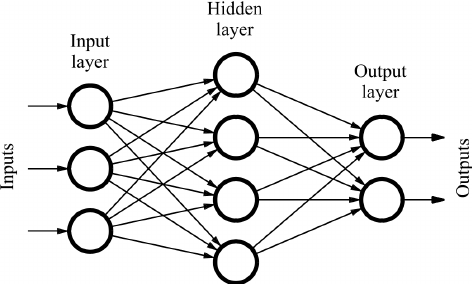
\includegraphics[width=0.9\textwidth]{images/ANN/ann.png}
    \caption{A feed forward neural network}
       \label{fig:ann}
\end{minipage}
\begin{minipage}[b]{0.5\textwidth}
\centering
    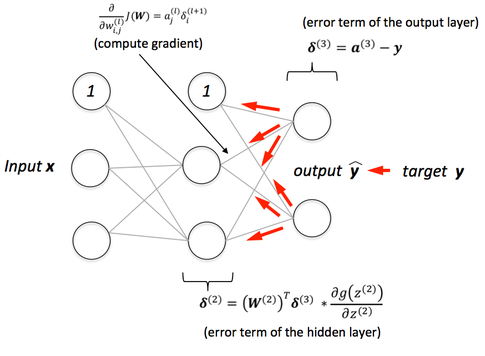
\includegraphics[width=0.9\textwidth]{images/ANN/backpropagation.png}
    \caption{BP algorithm (\cite{raschka})}
       \label{fig:bp}
\end{minipage}
\end{figure} 
Backpropagation learning algorithm (BP) aims at minimizing the error. Instead of just propagating the information forward, it back-propagates the error, calculate the gradient of the error function based on chain rule and finally update the weights (see figure \ref{fig:bp}). For regular back propagation, a small learning rate is normally used, which leads to the slow training process.
\\\\Resilient Propagation algorithm (Rprop) is an iterative process, which was developed in 1993 in an attempt to improve upon the BP algorithm. Unlike BP, Rprop  does not use the magnitude of the gradient; instead, it uses only the sign of the gradient and performs a local adaptation of the weight-updates (\cite{riedmiller1993direct}). Therefore, it is more efficient and flexible.

\subsubsection{Experimental Setup}
In this section, multilayer perceptron neural networks (MLP) are applied to predict the monthly tourist overnight stays in Austria from Jan 2011 to Nov 2017 by testing both traditional BP algorithm and Rprop+ algorithm. 
\begin{enumerate}
  \item Data Preprocessing
\\Data are scaled using Min-Max scaling method to make sure the minimum and maximum values of each time series map to the boundary [0,1]. Several ways of data processing have been considered. First, it's about whether to apply log-return or not. As it is shown in figure \ref{fig:hist}, several provinces have positiveskewness, however ANNs do not care much about distribution of data. Therefore, we use the raw data. 
\\Second, it is to decided whether to difference time series data or not. Previous experiments on predicting tourism data showed that ANN models trained by undifferenced data have better forecasting performance (\cite{taieb2014machine}). Therefore, in this case we do not difference it. 
\\Besides, \citeauthor{makridakis1982accuracy} (1982) found that forecast results from ANN models trained by deseasonlized data are significantly more accurate than those trained by non-deseasonalised data. Although in this paper non-deseasonalised data are used, deseasonalising can be a good way to improve the accuracy of model prediction.
  \item Neural Network Construction
  \begin{itemize}
    \item The Network Architecture
    \\Several factors need to be taken into consideration while designing a proper neural network. First, for the input layer, inputs are from three aspects: time delays data, monthly dummies and neighbourhoods’ time delays data. Therefore, for different models, the specific selections of input variables have slightly differences and the number of nodes ranges from at least 3 to more than \texttt{12(lags)+11(monthly dummies)+n*12(lags)} (where n is the number of first-order neighbours). 
    \\Second, for hidden layer, one layer is required in this case as previous findings suggest one is enough for time series forecasting (\cite{dong2013one}). The number of hidden nodes is decided through experiments, and the final optimal size of hidden layer varies for each province. 
    \\Third, for output layer, the number of neurons is one, i.e. the output is the predicted next month overnight stays.
    \item The Error and Activation Function
    \\The error function is sum of squared error (\texttt{SSE}) which is used to compare predicted values and outcome values and help generate new weights with learning rate during the training procedure. Activation function for the hidden layer is a sigmoid transfer function (\texttt{Logistic}) which is suggested by Klimasauskas who found it is better than the hyperbolic tangent function when learning the average behaviour. Finally, linear function is the activation function for output layer.
    \item The Stopping Criteria
    \\Late stopping is one way to stop training iteration when a certain error condition is achieved. For traditional BP method, we set \texttt{maxit} parameter to 1000 through nnet package; for Rprop+ method, we set \texttt{threshold} to 0.01 and \texttt{maxstep} to 1e5 through nerualnet package as stopping conditions.
    \item Performance Measures
    \\For each model, it will be trained several times and the optimal outcome model will be selected. Corresponding control parameters for training times are \texttt{repeats} and \texttt{rep} for the two methods, respectively. In this case, we use RMSE as the performance measure.
  \end{itemize}
\end{enumerate}
\subsubsection{Model Selection and Results} 
\begin{enumerate}
    \item Different Algorithms and Parameter Combinations
    \\For traditional back-propagation, grid search of both \texttt{size} and \texttt{decay} is needed; Here, the number of hidden nodes are ranged in the set \{5,7,9\} and weight decay possible values are from the following options \{0.1,0.5,0.7,1\}. The selected parameters are made based on a broader range of grid search, of which results are not presented.
\\
The best tune varies for different provinces (see table \ref{tab:nnet_besttune}), for example, as for model of Corinthian, the optimal hidden nodes and weight decay are 5 and 1 respectively (see figure \ref{fig:nn_besttune}). The overall performance of BP models is good, except for Vienna whose model can only explain 78.9\% of the response variability. 
Therefore, Rprop algorithm is introduced to see if it can improve the model. For this method, learning rate is not required to be specified. Thus, the only task is to find a proper number of hidden nodes. Generally, the increase of hidden neurons will help improve the accuracy of model. However, the problem is more computing time and danger of over fitting. 
\\
Here, we set the maximum hidden nodes number to 12 which equals to the basic inputs 12 time lags and the minimum number is 6. In figure \ref{fig:dhn_neural}, each model is the optimal one from 35 repetitions and it can be seen that there is no much difference among models with different numbers of hidden nodes for most provinces and it does not follow the common sense that the more nodes the better fit either. Besides, Styria and Vienna are the probably the top two models which are hard to fit because their results are more discrete than others. Table \ref{tab:rprop_dhn} shows the results of RMSE and R Square of the models and Vienna's R Square improves to 94.5\%. From figure \ref{fig:nn_vienna}, it can be seen clearly that in the BP model Vienna has a bad fit with the problem of not catching up the growing trend while the Rprop model performs very well. It suggests that Rprop may be more able to update weights through learning past errors than traditional BP. Hence, we adopt Rprop algorithm for the following analysis.
\begin{figure}[H]
	\begin{minipage}[b]{0.5\textwidth}
      \centering
    \begin{tabular}{lcccc}
    \toprule
    & \multicolumn{1}{l}{\textbf{Size}} & \multicolumn{1}{l}{\textbf{Decay}} & \multicolumn{1}{l}{\textbf{RMSE}} & \multicolumn{1}{l}{\textbf{R Square}} \\
    \midrule
    Burgenland & 5     & 0.1   & 19948 & 0.9702 \\
    Carinthia & 5     & 1     & 92357 & 0.9882 \\
    LowerAustria & 5     & 0.3   & 25756 & 0.9761 \\
    UpperAustria & 5     & 1     & 39680 & 0.9772 \\
    Salzburg & 5     & 1     & 242359 & 0.9649 \\
    Styria & 9     & 1     & 59874 & 0.9676 \\
    Tyrol & 9     & 1     & 396216 & 0.9629 \\
    Vorarlberg & 9     & 0.2   & 87849 & 0.9489 \\
    Vienna & 9     & 0.3   & 243918 & 0.7892 \\
    \bottomrule
    \end{tabular}
   \captionof{table}{The Results of Best Tune for Transitional BP}
   \label{tab:nnet_besttune}
\end{minipage}
\begin{minipage}[b]{0.5\textwidth}
\centering
    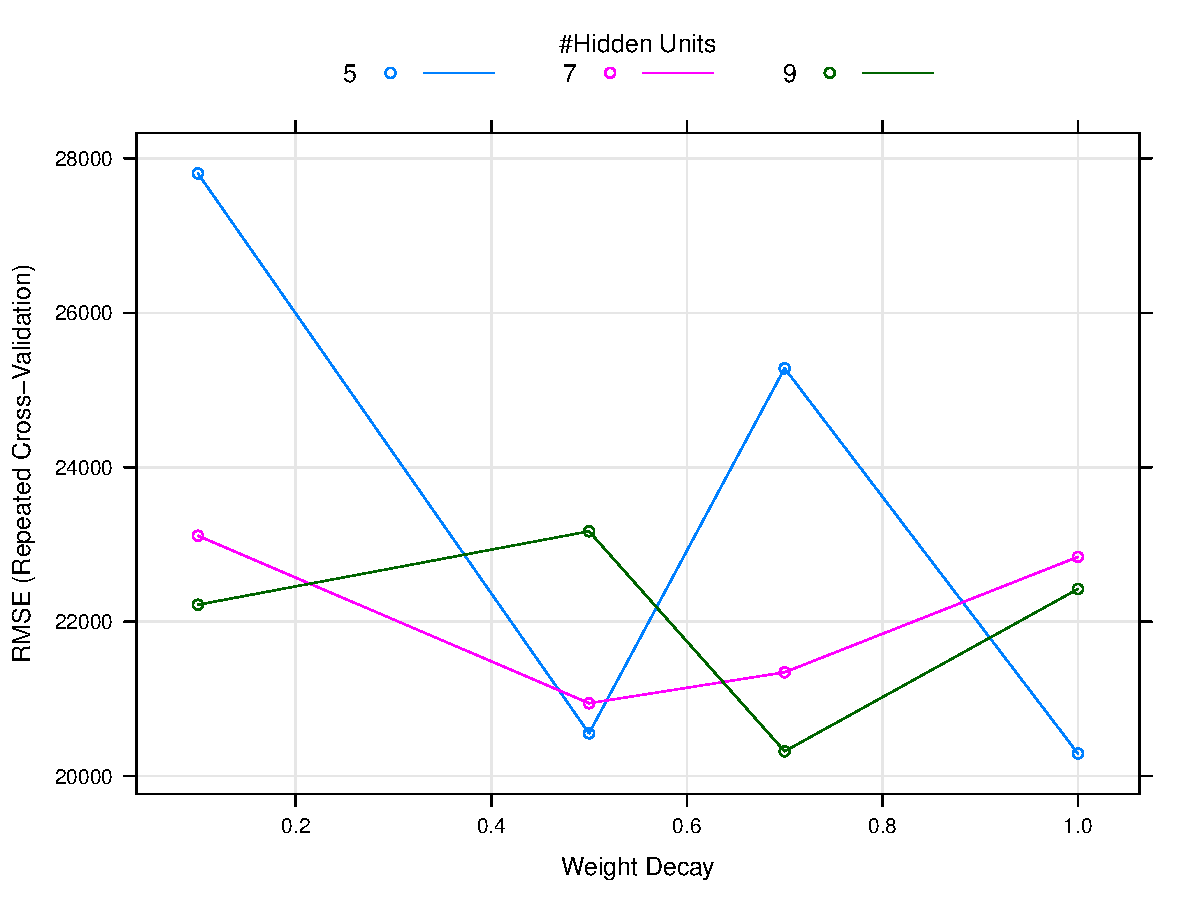
\includegraphics[clip,trim=0cm 0.3cm 0cm 0cm,width=0.9\textwidth]{images/ANN/nnet_grid_search.pdf}
    \captionof{figure}{Example of Grid Search for BP}
       \label{fig:nn_besttune}
\end{minipage}
\end{figure}

\begin{figure}[H]
\begin{minipage}[b]{0.9\textwidth}
\centering
  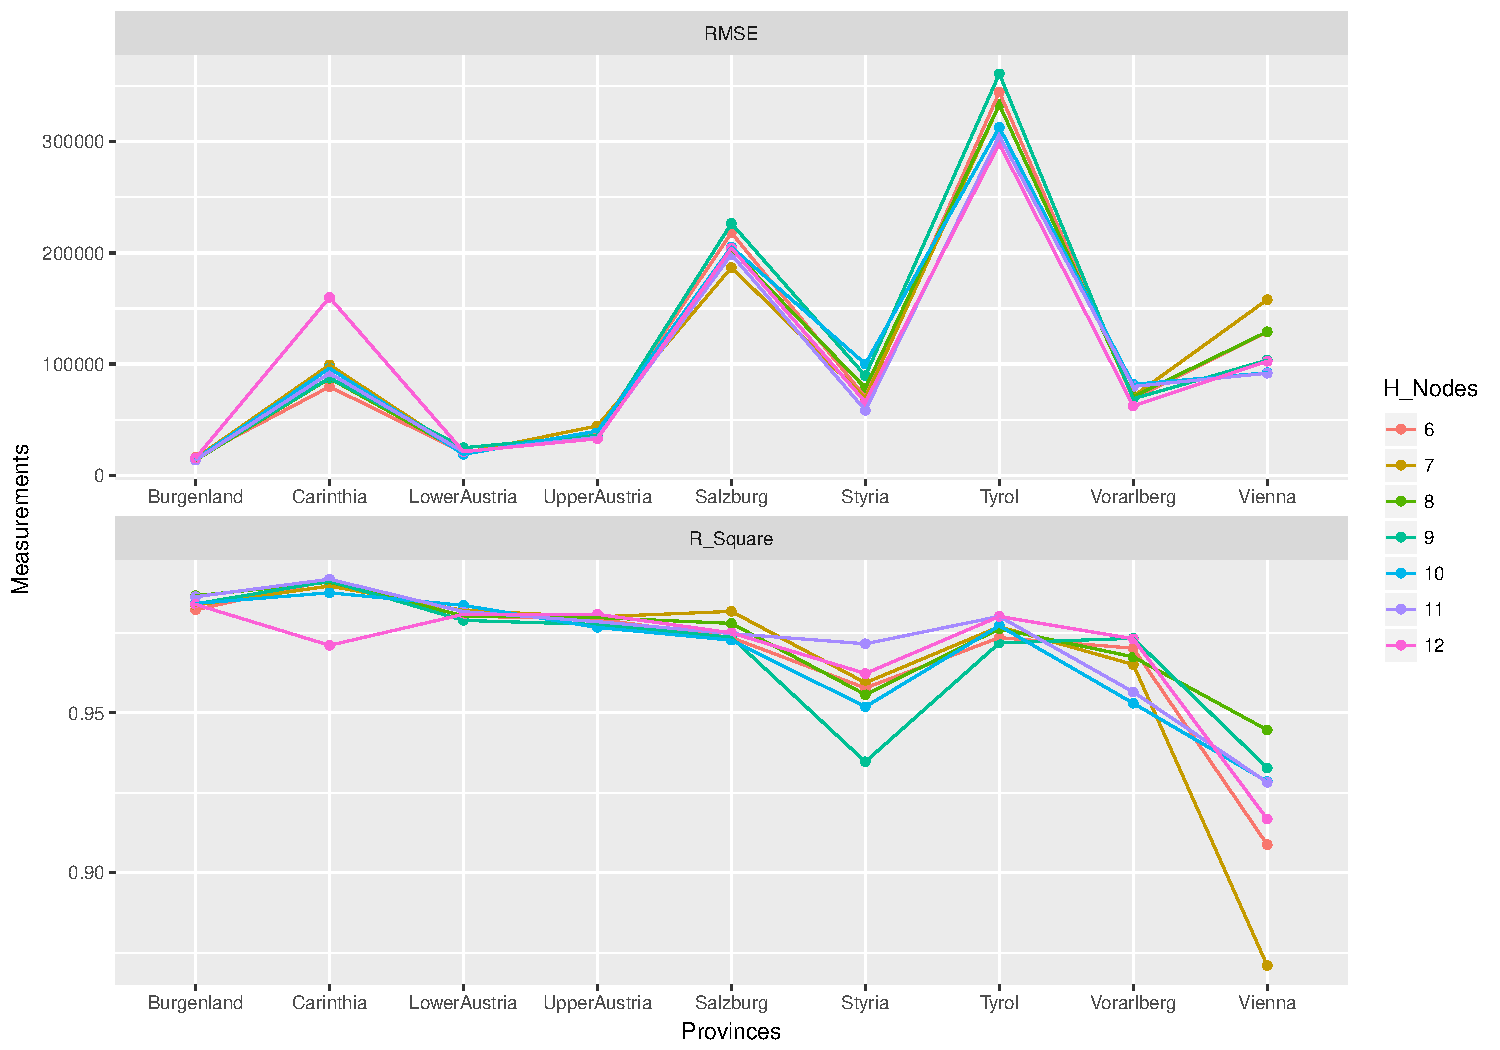
\includegraphics[width=1\textwidth]{images/ANN/dnh_new.pdf}
    \captionof{figure}{Different Hidden Nodes Comparison for Rprop+}
       \label{fig:dhn_neural}
\end{minipage}
\end{figure}

\begin{table}[H]
  \centering
	\small
    \begin{tabular}{cccccccccc}
    \toprule
          & Burgenland & Carinthia & L.Austria & U.Austria & Salzburg & Styria & Tyrol & Vorarlberg & Vienna \\
    \midrule
    \textbf{H.Nodes} & 8     & 6     & 10    & 12    & 7     & 11    & 12    & 12    & 11 \\
    \textbf{$R^{2}$}    & \cellcolor[rgb]{ .984,  .922,  .933}0.9866 & \cellcolor[rgb]{ .988,  .988,  1}0.9918 & \cellcolor[rgb]{ .984,  .886,  .898}0.9836 & \cellcolor[rgb]{ .984,  .851,  .863}0.9808 & \cellcolor[rgb]{ .984,  .863,  .875}0.9817 & \cellcolor[rgb]{ .98,  .741,  .749}0.9716 & \cellcolor[rgb]{ .984,  .843,  .855}0.9802 & \cellcolor[rgb]{ .98,  .757,  .769}0.9731 & \cellcolor[rgb]{ .973,  .412,  .42}0.9447 \\
    \textbf{RMSE}  & \cellcolor[rgb]{ .988,  .988,  1}13593 & \cellcolor[rgb]{ .988,  .855,  .867}79649 & \cellcolor[rgb]{ .988,  .98,  .992}18865 & \cellcolor[rgb]{ .988,  .953,  .961}32830 & \cellcolor[rgb]{ .98,  .639,  .647}186846 & \cellcolor[rgb]{ .988,  .898,  .91}58431 & \cellcolor[rgb]{ .973,  .412,  .42}298194 & \cellcolor[rgb]{ .988,  .89,  .902}62224 & \cellcolor[rgb]{ .984,  .831,  .843}91772 \\    
    \bottomrule
    \end{tabular}
\caption{The Results of Best Hidden Nodes for Rprop+}
\label{tab:rprop_dhn}
\end{table}
\begin{figure}[H]
\begin{minipage}[b]{0.49\textwidth}
\centering    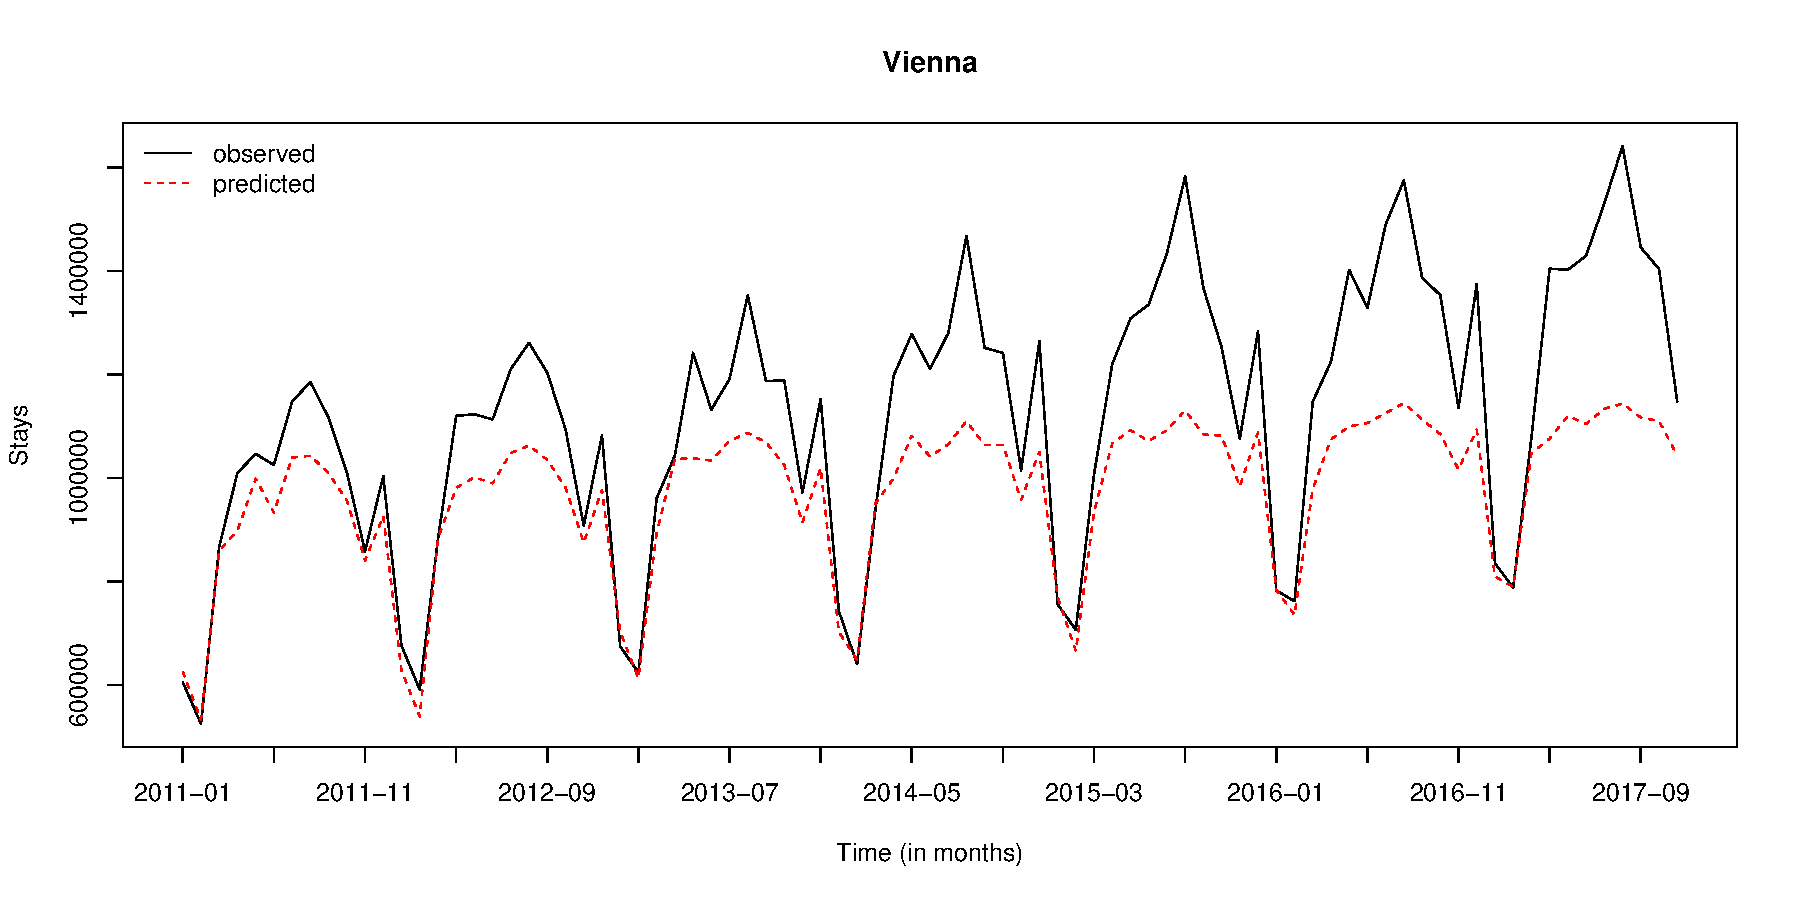
\includegraphics[width=\textwidth]{images/ANN/nnet_Vienna_.pdf}
\end{minipage}
\begin{minipage}[b]{0.49\textwidth}
\centering    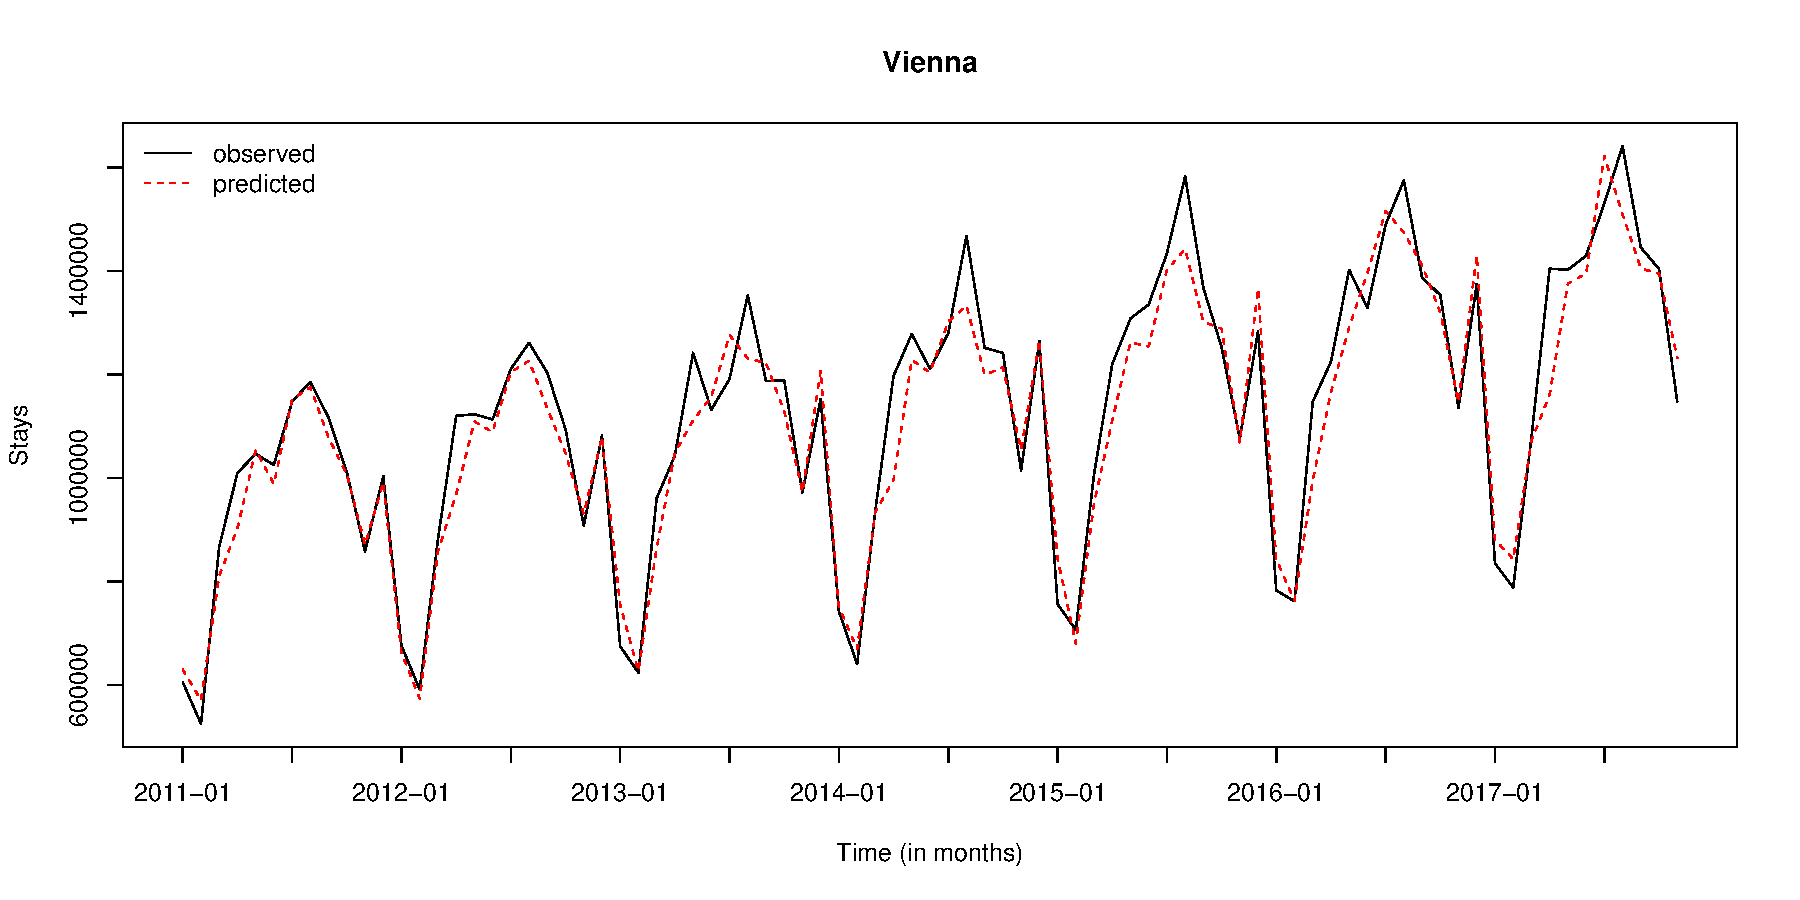
\includegraphics[width=\textwidth]{images/ANN/neural_Vienna_.pdf}  
\end{minipage}
\captionof{figure}{Observed data vs Predicted data of Vienna (Left: Traditional BP; Right: Rprop+)}
\label{fig:nn_vienna}
\end{figure}
    \item Different Training Data Lengths
    \\Different training data lengths are tested in this section to see its effect on the accuracy of models, namely 5-year length, 10-year length, 20-year length and total 36 years. Among all the results (see table \ref{tab:ann_dtl}), the full range data length model performs the best. However, it takes more time than shorter length ones. Therefore, if accuracy and time consuming are both considered, mid length of training data would be a better option.  
\begin{table}[H]
  \centering
  \small
    \begin{tabular}{lccccccccc}
    \toprule
    & Burgenland & Carinthia & L.Austria & U.Austria & Salzburg & Styria & Tyrol & Vorarlberg & Vienna \\
    \midrule
    \textbf{RMSE}  &       &       &       &       &       &       &       &       &  \\
    2005-2010 & \cellcolor[rgb]{ .988,  .988,  1}18095 & \cellcolor[rgb]{ .988,  .988,  1}92919 & \cellcolor[rgb]{ .988,  .988,  1}25507 & \cellcolor[rgb]{ .988,  .988,  1}34177 & \cellcolor[rgb]{ .988,  .988,  1}236439 & \cellcolor[rgb]{ .988,  .988,  1}69594 & \cellcolor[rgb]{ .988,  .988,  1}345634 & \cellcolor[rgb]{ .906,  .953,  .925}81304 & \cellcolor[rgb]{ .988,  .988,  1}116732 \\
    \multicolumn{1}{c}{2000-2010} & \cellcolor[rgb]{ .447,  .769,  .533}13580 & \cellcolor[rgb]{ .388,  .745,  .482}79112 & \cellcolor[rgb]{ .49,  .784,  .569}20003 & \cellcolor[rgb]{ .388,  .745,  .482}31319 & \cellcolor[rgb]{ .388,  .745,  .482}174364 & \cellcolor[rgb]{ .388,  .745,  .482}52095 & \cellcolor[rgb]{ .878,  .941,  .906}337064 & \cellcolor[rgb]{ .749,  .89,  .792}75572 & \cellcolor[rgb]{ .396,  .745,  .486}70609 \\
    1990-2010 & \cellcolor[rgb]{ .388,  .745,  .482}13078 & \cellcolor[rgb]{ .416,  .753,  .506}79774 & \cellcolor[rgb]{ .576,  .82,  .643}20968 & \cellcolor[rgb]{ .859,  .937,  .89}33579 & \cellcolor[rgb]{ .804,  .914,  .843}217653 & \cellcolor[rgb]{ .765,  .898,  .808}63125 & \cellcolor[rgb]{ .518,  .796,  .592}308482 & \cellcolor[rgb]{ .988,  .988,  1}84324 & \cellcolor[rgb]{ .388,  .745,  .482}69924 \\
    1973-2010 & \cellcolor[rgb]{ .447,  .769,  .533}13593 & \cellcolor[rgb]{ .408,  .753,  .502}79649 & \cellcolor[rgb]{ .388,  .745,  .482}18865 & \cellcolor[rgb]{ .702,  .871,  .753}32830 & \cellcolor[rgb]{ .506,  .792,  .584}186846 & \cellcolor[rgb]{ .604,  .831,  .667}58431 & \cellcolor[rgb]{ .388,  .745,  .482}298194 & \cellcolor[rgb]{ .388,  .745,  .482}62224 & \cellcolor[rgb]{ .667,  .855,  .722}91772 \\
    \midrule
	\textbf{R Square} &       &       &       &       &       &       &       &       &  \\
    2005-2010 & \cellcolor[rgb]{ .988,  .988,  1}0.9795 & \cellcolor[rgb]{ .988,  .988,  1}0.9882 & \cellcolor[rgb]{ .922,  .961,  .945}0.9814 & \cellcolor[rgb]{ .976,  .984,  .992}0.9781 & \cellcolor[rgb]{ .988,  .988,  1}0.9683 & \cellcolor[rgb]{ .988,  .988,  1}0.9609 & \cellcolor[rgb]{ .988,  .988,  1}0.9744 & \cellcolor[rgb]{ .929,  .965,  .949}0.9612 & \cellcolor[rgb]{ .988,  .988,  1}0.9152 \\
    \multicolumn{1}{c}{2000-2010} & \cellcolor[rgb]{ .471,  .78,  .553}0.9866 & \cellcolor[rgb]{ .396,  .749,  .49}0.9917 & \cellcolor[rgb]{ .988,  .988,  1}0.9811 & \cellcolor[rgb]{ .714,  .878,  .765}0.9793 & \cellcolor[rgb]{ .463,  .776,  .549}0.9801 & \cellcolor[rgb]{ .388,  .745,  .482}0.9727 & \cellcolor[rgb]{ .914,  .961,  .937}0.9751 & \cellcolor[rgb]{ .965,  .98,  .98}0.9604 & \cellcolor[rgb]{ .478,  .784,  .561}0.9471 \\
    1990-2010 & \cellcolor[rgb]{ .388,  .745,  .482}0.9877 & \cellcolor[rgb]{ .514,  .796,  .588}0.9911 & \cellcolor[rgb]{ .91,  .957,  .933}0.9815 & \cellcolor[rgb]{ .988,  .988,  1}0.9781 & \cellcolor[rgb]{ .745,  .89,  .792}0.9737 & \cellcolor[rgb]{ .718,  .878,  .769}0.9663 & \cellcolor[rgb]{ .604,  .831,  .667}0.9781 & \cellcolor[rgb]{ .988,  .988,  1}0.9598 & \cellcolor[rgb]{ .388,  .745,  .482}0.9526 \\
    1973-2010 & \cellcolor[rgb]{ .467,  .776,  .549}0.9866 & \cellcolor[rgb]{ .388,  .745,  .482}0.9918 & \cellcolor[rgb]{ .388,  .745,  .482}0.9836 & \cellcolor[rgb]{ .388,  .745,  .482}0.9808 & \cellcolor[rgb]{ .388,  .745,  .482}0.9817 & \cellcolor[rgb]{ .447,  .773,  .533}0.9716 & \cellcolor[rgb]{ .388,  .745,  .482}0.9802 & \cellcolor[rgb]{ .388,  .745,  .482}0.9731 & \cellcolor[rgb]{ .518,  .8,  .596}0.9447 \\
    \bottomrule
    \end{tabular}
  \caption{The Results for Models with Different Training Length}
  \label{tab:ann_dtl}
\end{table}
    \item Different Ways of Incorporating Spatial-Temporal Information
    \\In this part, the effect of different length of lagged terms, monthly dummies and spatial adjacency matrix on ANN models are tested. First, we compare the test results of models with 4 different lengths lags and whether including monthly variables or not. It can be seen from table \ref{tab:lags and dummies} that in most cases as the length of lagged term increases,  the RMSE of the test set reduces, except for Vienna, for which the best predictor combination is one lag term (\texttt{Lag.1}) with monthly variables. One more finding is that by adding monthly dummies the average running time of models gets shorter. Therefore, based on the results, models in following sections will still use Lag.1-Lag.12 as inputs but adding monthly dummies for models of Vorarlberg.
    \begin{table}[H]
      \centering
        \begin{tabular}{lcccccccc}
        \toprule
         & \multicolumn{4}{c}{Without Monthly Dummies} & \multicolumn{4}{c}{With Monthly Dummies} \\
         \cmidrule(lr){2-5}\cmidrule(lr){6-9}
         & \multicolumn{1}{l}{Lag.1} & \multicolumn{1}{l}{Lag.1 - 3} & \multicolumn{1}{l}{Lag.1 - 6} & \multicolumn{1}{l}{Lag.1 - 12} & \multicolumn{1}{l}{Lag.1} & \multicolumn{1}{l}{Lag.1 - 3} & \multicolumn{1}{l}{Lag.1 - 6} & \multicolumn{1}{l}{Lag.1 - 12} \\
        \midrule
        Burgenland & \cellcolor[rgb]{ .973,  .412,  .42}58,017 & \cellcolor[rgb]{ .992,  .776,  .49}34,360 & \cellcolor[rgb]{ 1,  .882,  .51}27,601 & \cellcolor[rgb]{ .388,  .745,  .482}16,150 & \cellcolor[rgb]{ 1,  .914,  .518}25,499 & \cellcolor[rgb]{ .949,  .906,  .514}24,086 & \cellcolor[rgb]{ .824,  .871,  .506}22,329 & \cellcolor[rgb]{ .478,  .769,  .486}17,472 \\
        Carinthia & \cellcolor[rgb]{ .973,  .412,  .42}1,328,152 & \cellcolor[rgb]{ 1,  .871,  .51}302,405 & \cellcolor[rgb]{ 1,  .886,  .514}269,274 & \cellcolor[rgb]{ .408,  .749,  .482}90,509 & \cellcolor[rgb]{ 1,  .918,  .518}203,132 & \cellcolor[rgb]{ .906,  .894,  .51}172,948 & \cellcolor[rgb]{ .89,  .89,  .51}170,179 & \cellcolor[rgb]{ .388,  .745,  .482}86,730 \\
        L.Austria & \cellcolor[rgb]{ .973,  .412,  .42} 91,319 & \cellcolor[rgb]{ .992,  .773,  .49}60,552 & \cellcolor[rgb]{ .996,  .918,  .514}47,387 & \cellcolor[rgb]{ .388,  .745,  .482}23,526 & \cellcolor[rgb]{ 1,  .906,  .518}48,878 & \cellcolor[rgb]{ 1,  .922,  .518}47,433 & \cellcolor[rgb]{ .914,  .894,  .51}44,097 & \cellcolor[rgb]{ .416,  .753,  .482}24,621 \\
        U.Austria & \cellcolor[rgb]{ .973,  .412,  .42}164,841 & \cellcolor[rgb]{ .992,  .718,  .478}96,655 & \cellcolor[rgb]{ .996,  .824,  .502}72,302 & \cellcolor[rgb]{ .592,  .804,  .494}32,486 & \cellcolor[rgb]{ .996,  .784,  .494}81,688 & \cellcolor[rgb]{ 1,  .918,  .518}51,534 & \cellcolor[rgb]{ 1,  .914,  .518}52,333 & \cellcolor[rgb]{ .722,  .839,  .498}38,162 \\
        Salzburg & \cellcolor[rgb]{ .973,  .412,  .42}1,024,971 & \cellcolor[rgb]{ .996,  .8,  .494}438,376 & \cellcolor[rgb]{ 1,  .89,  .514}301,256 & \cellcolor[rgb]{ .388,  .745,  .482}226,987 & \cellcolor[rgb]{ .898,  .89,  .51}246,001 & \cellcolor[rgb]{ .702,  .835,  .498}238,687 & \cellcolor[rgb]{ .961,  .91,  .514}248,339 & \cellcolor[rgb]{ 1,  .922,  .518}251,169 \\
        Styria & \cellcolor[rgb]{ .973,  .412,  .42}286,442 & \cellcolor[rgb]{ .976,  .463,  .431}270,685 & \cellcolor[rgb]{ .992,  .733,  .482}180,891 & \cellcolor[rgb]{ .388,  .745,  .482}84,232 & \cellcolor[rgb]{ 1,  .875,  .51}133,905 & \cellcolor[rgb]{ .69,  .831,  .498}100,652 & \cellcolor[rgb]{ .58,  .8,  .49}94,616 & \cellcolor[rgb]{ .612,  .808,  .494}96,439 \\
        Tyrol & \cellcolor[rgb]{ .973,  .412,  .42}1,694,054 & \cellcolor[rgb]{ .996,  .804,  .498}738,074 & \cellcolor[rgb]{ 1,  .89,  .514}528,695 & \cellcolor[rgb]{ .424,  .753,  .482}339,196 & \cellcolor[rgb]{ 1,  .914,  .518}471,150 & \cellcolor[rgb]{ .878,  .886,  .51}426,453 & \cellcolor[rgb]{ .886,  .886,  .51}428,527 & \cellcolor[rgb]{ .388,  .745,  .482}331,747 \\
        Vorarlberg & \cellcolor[rgb]{ .973,  .412,  .42}330,423 & \cellcolor[rgb]{ .996,  .812,  .498}176,804 & \cellcolor[rgb]{ .643,  .816,  .494}98,707 & \cellcolor[rgb]{ .588,  .8,  .49}93,522 & \cellcolor[rgb]{ .918,  .898,  .51}125,734 & \cellcolor[rgb]{ 1,  .902,  .518}141,446 & \cellcolor[rgb]{ .992,  .757,  .486}198,356 & \cellcolor[rgb]{ .388,  .745,  .482}73,532 \\
        Vienna & \cellcolor[rgb]{ .973,  .412,  .42}243,420 & \cellcolor[rgb]{ .98,  .518,  .443}228,745 & \cellcolor[rgb]{ .996,  .824,  .502}185,026 & \cellcolor[rgb]{ .996,  .847,  .506}181,462 & \cellcolor[rgb]{ .388,  .745,  .482}86,786 & \cellcolor[rgb]{ .918,  .898,  .51}159,606 & \cellcolor[rgb]{ .867,  .882,  .51}152,804 & \cellcolor[rgb]{ .878,  .886,  .51}154,390 \\
        \bottomrule
        \end{tabular}%
      \caption{Test RMSE Results Comparison}
      \label{tab:lags and dummies}%
    \end{table}%
The following table \ref{tab:ann_st_result} shows the results of STANN models by adding first-order neighbours' time lags as inputs. The result does not show much improvement of accuracy compared to previous models probably due to the weak spatial autocorrelation based on spatial adjacency matrix. 
\begin{table}[H]
  \centering \small
    \begin{tabular}{cccccccccc}
    \toprule
          & Burgenland & Carinthia & L.Austria & U.Austria & Salzburg & Styria & Tyrol & Vorarlberg & Vienna \\
    \midrule    
    \textbf{$R^{2}$} & \cellcolor[rgb]{ .988,  .988,  1}0.9795 & \cellcolor[rgb]{ .984,  .945,  .957}0.9748 & \cellcolor[rgb]{ .98,  .808,  .82}0.9600 & \cellcolor[rgb]{ .984,  .941,  .953}0.9744 & \cellcolor[rgb]{ .984,  .91,  .922}0.9711 & \cellcolor[rgb]{ .976,  .588,  .596}0.9359 & \cellcolor[rgb]{ .984,  .855,  .863}0.9650 & \cellcolor[rgb]{ .984,  .871,  .882}0.9669 & \cellcolor[rgb]{ .973,  .412,  .42}0.9164 \\
    \textbf{RMSE}  & \cellcolor[rgb]{ .988,  .988,  1}16,610 & \cellcolor[rgb]{ .984,  .812,  .824}138,396 & \cellcolor[rgb]{ .988,  .969,  .98}31,072 & \cellcolor[rgb]{ .988,  .957,  .969}39,717 & \cellcolor[rgb]{ .984,  .722,  .729}202,805 & \cellcolor[rgb]{ .988,  .882,  .894}91,163 & \cellcolor[rgb]{ .973,  .412,  .42}413,935 & \cellcolor[rgb]{ .988,  .906,  .918}73,773 & \cellcolor[rgb]{ .988,  .886,  .898}87,763 \\
    \bottomrule
    \end{tabular}%
  \caption{Results for Spatio-Temporal ANN Models.}
  \label{tab:ann_st_result}%
\end{table}%
    
    \item Different Forecasting Horizons
    \\One-step ahead prediction (see figure \ref{fig:1step_ann}) and multi-step ahead prediction methods are adopted for forecasting. There are two different forecasting horizons: the long one is about seven years while the short one is only for one year. Usually, short term prediction can reach a higher accuracy (see table \ref{tab:ann_nstep_result}). However, for Burgenland and Vorarlberg long term one-step ahead prediction performs even better than short term prediction, which may indicate the ANN models are well trained. For short term prediction, the two methods do not have obvious differences but for long-term forecasting, multi-step ahead models produce a low performance in some provinces like Upper Austria and Vienna (see figure \ref{fig:nstep_ann}).  It is possibly because ANNs is sensitive to the accumulation of errors for the long term forecasting horizon. 

\begin{table}[H]
  \centering
  \small
    \begin{tabular}{cccccccccc}
    \toprule
    & Burgenland & Carinthia & L.Austria & U.Austria & Salzburg & Styria & Tyrol & Vorarlberg & Vienna \\
    \midrule
    \multicolumn{2}{l}{\textbf{1-step ahead}} &       &       &       &       &       &       &       &  \\
    2010-2017 & \cellcolor[rgb]{ .388,  .745,  .482}0.9876 & \cellcolor[rgb]{ .988,  .988,  1}0.9917 & \cellcolor[rgb]{ .988,  .988,  1}0.9831 & \cellcolor[rgb]{ .988,  .988,  1}0.9821 & \cellcolor[rgb]{ .988,  .988,  1}0.9806 & \cellcolor[rgb]{ .988,  .988,  1}0.9682 & \cellcolor[rgb]{ .988,  .988,  1}0.9792 & \cellcolor[rgb]{ .388,  .745,  .482}0.9759 & \cellcolor[rgb]{ .988,  .988,  1}0.9545 \\
    2010-2011 & \cellcolor[rgb]{ .988,  .988,  1}0.9861 & \cellcolor[rgb]{ .388,  .745,  .482}0.9947 & \cellcolor[rgb]{ .388,  .745,  .482}0.9984 & \cellcolor[rgb]{ .388,  .745,  .482}0.9928 & \cellcolor[rgb]{ .388,  .745,  .482}0.9877 & \cellcolor[rgb]{ .388,  .745,  .482}0.9749 & \cellcolor[rgb]{ .388,  .745,  .482}0.9866 & \cellcolor[rgb]{ .988,  .988,  1}0.9759 & \cellcolor[rgb]{ .388,  .745,  .482}0.9683 \\
    \midrule
    \multicolumn{2}{l}{\textbf{Multi-step ahead}} &       &       &       &       &       &       &       &  \\
    2010-2017 & \cellcolor[rgb]{ .988,  .988,  1}0.9618 & \cellcolor[rgb]{ .988,  .988,  1}0.9738 & \cellcolor[rgb]{ .988,  .988,  1}0.9736 & \cellcolor[rgb]{ .988,  .988,  1}0.9580 & \cellcolor[rgb]{ .988,  .988,  1}0.9681 & \cellcolor[rgb]{ .988,  .988,  1}0.9108 & \cellcolor[rgb]{ .988,  .988,  1}0.9750 & \cellcolor[rgb]{ .988,  .988,  1}0.9633 & \cellcolor[rgb]{ .988,  .988,  1}0.7352 \\
   2010-2011 & \cellcolor[rgb]{ .388,  .745,  .482}0.9721 & \cellcolor[rgb]{ .388,  .745,  .482}0.9936 & \cellcolor[rgb]{ .388,  .745,  .482}0.9975 & \cellcolor[rgb]{ .388,  .745,  .482}0.9939 & \cellcolor[rgb]{ .388,  .745,  .482}0.9846 & \cellcolor[rgb]{ .388,  .745,  .482}0.9777 & \cellcolor[rgb]{ .388,  .745,  .482}0.9865 & \cellcolor[rgb]{ .388,  .745,  .482}0.9637 & \cellcolor[rgb]{ .388,  .745,  .482}0.9695 \\
  \bottomrule
  \end{tabular}%
  \caption{R Square Results of One- and Multi-Step Ahead Prediction Models with Different Forecasting Horizons. Green Means Higher R Square Value.}
  \label{tab:ann_nstep_result}%
\end{table}%
\end{enumerate}
\subsubsection{Summary and Discussion}
In conclusion, a number of MLP networks were obtained on basis of combining the following factors: different training range (4), the number of input nodes (8); with or without spatial information (1), the number of hidden nodes (6), and forecasting horizons (2). Generally, all models perform well but still different neural models with different combinations of input variables perform differently. In this article, lagged terms are chosen following a common approach in the literature (e.g. t-1, t-2, t-3). However, in the future, models can be improved through identifying a set of key important inputs by introducing feature selection techniques.
To sum up, there is no formal method to build ANN models neither no standard criteria of the optimal number of hidden nodes. Therefore it is very necessary to do several experiments and repeat a certain times to get a proper result. 
\begin{figure}[H]
\begin{minipage}[b]{\textwidth}
\centering
  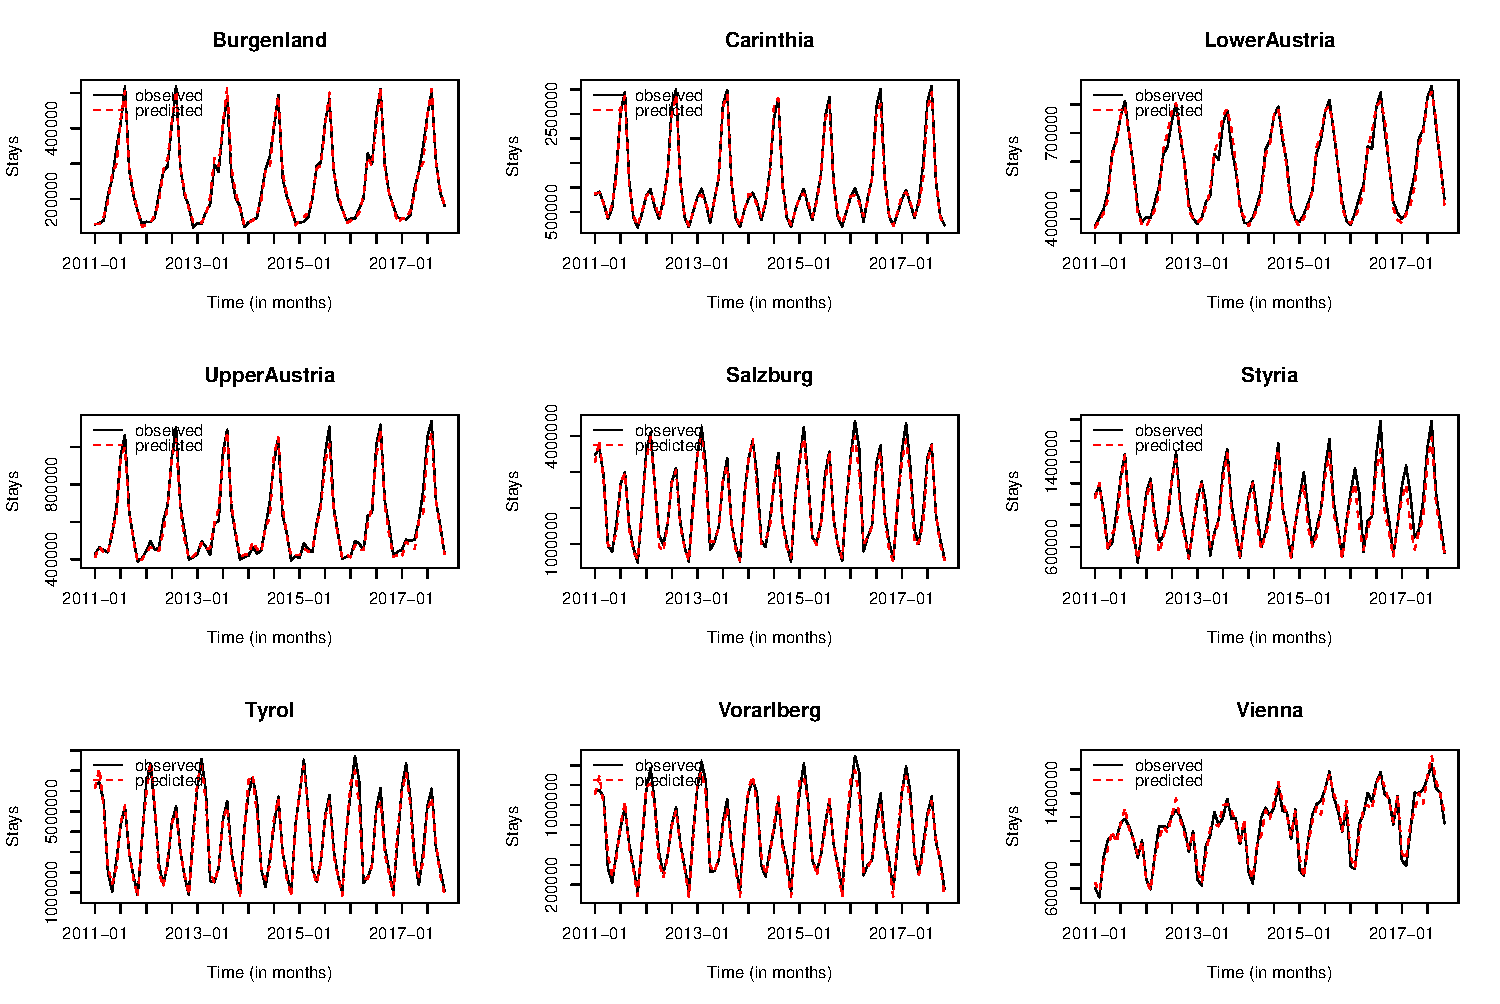
\includegraphics[width=0.9\textwidth]{images/ANN/oneahead_9final.pdf}
    \captionof{figure}{One-Step Ahead Prediction}
       \label{fig:1step_ann}
\end{minipage}
\end{figure}

\begin{figure}[H]
\begin{minipage}[b]{0.5\textwidth}
\centering
  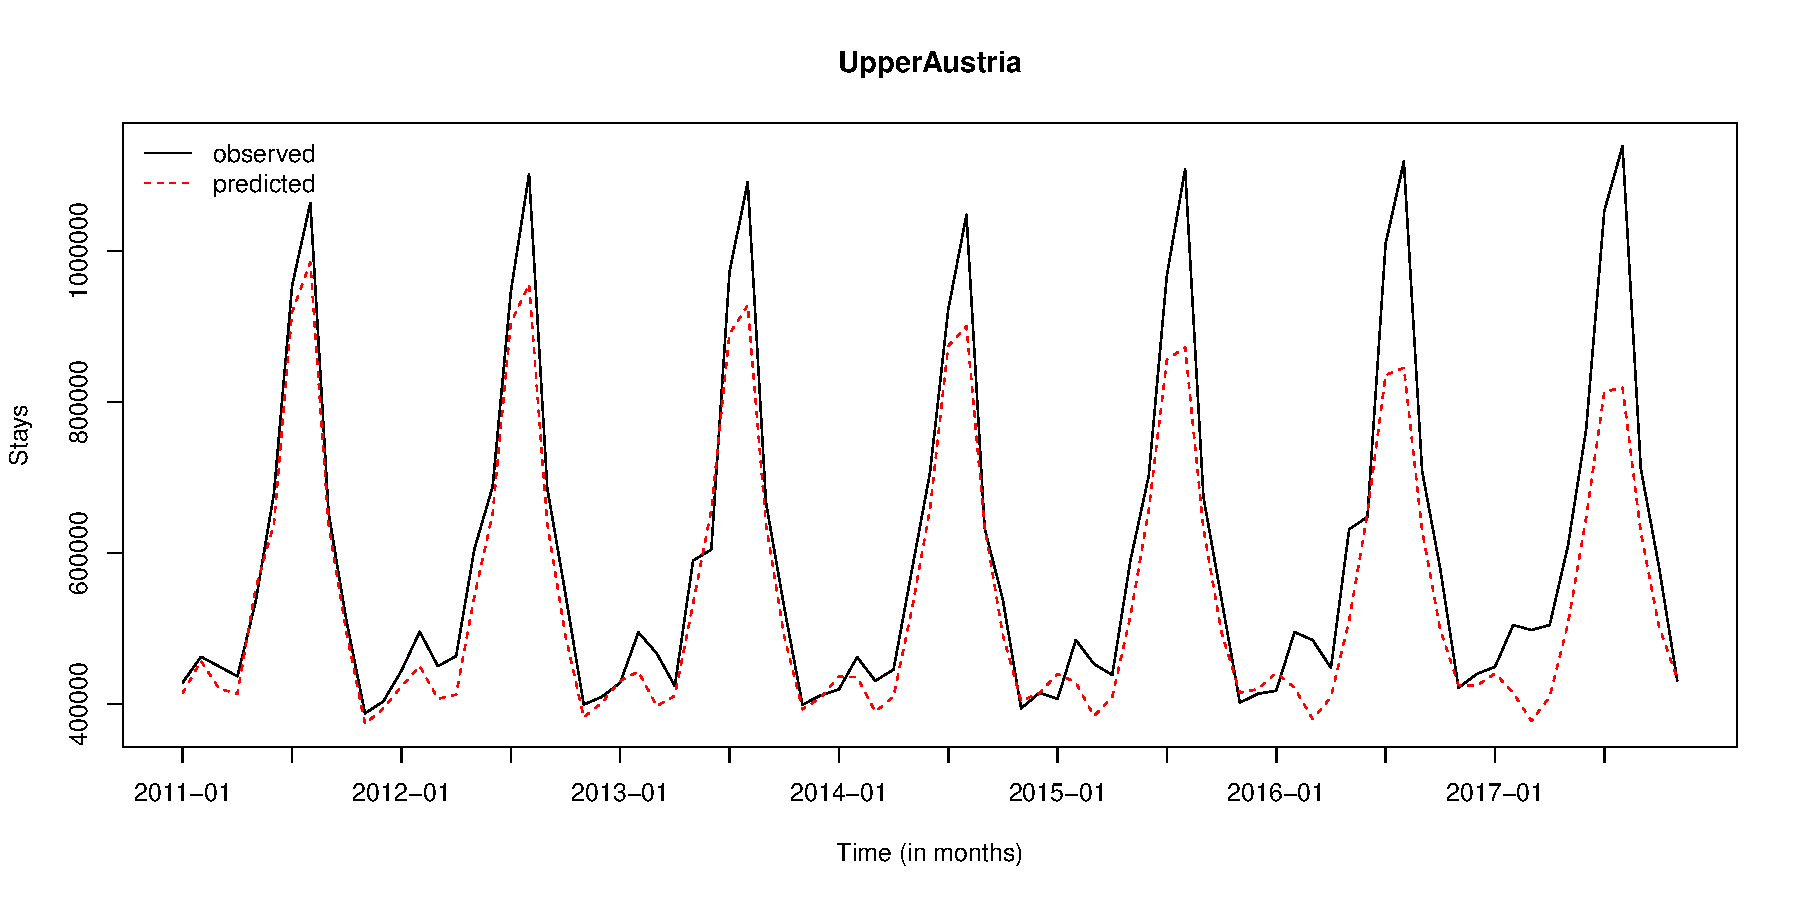
\includegraphics[width=\textwidth]
  {images/ANN/4_UpperAustria_.pdf}
\end{minipage}
\begin{minipage}[b]{0.5\textwidth}
\centering
  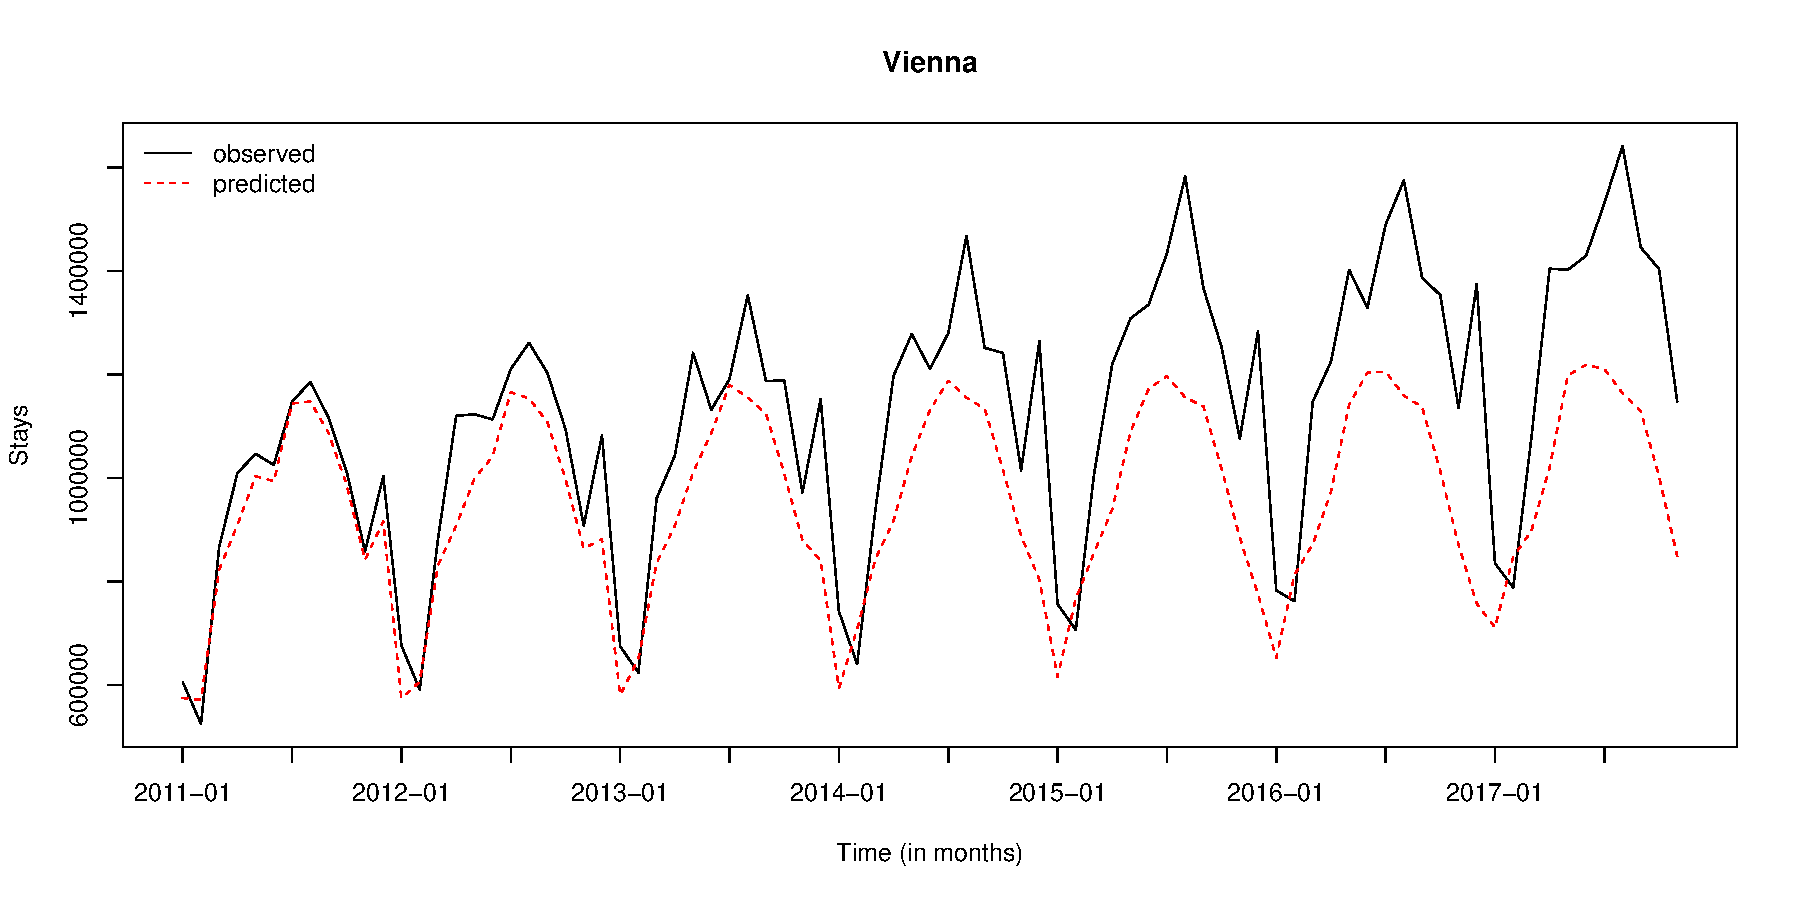
\includegraphics[width=\textwidth]{images/ANN/9_Vienna_.pdf}
\end{minipage}
\captionof{figure}{N-Step Ahead Prediction}
       \label{fig:nstep_ann}
\end{figure}


 
\newpage
\subsection{Support Vector Machine}
\label{ssec:svm}
\fancyhead[R]{Methods: SVM}
\subsubsection{Methodology}
Support Vector Machine (SVM) is a powerful machine learning method usually related to classification. However this could also be effectively used for regression. Here the regression mode also known as Support Vector Regression or SVR is used to predict the total night stays of tourist for each provinces in Austria using historical data.  SVR was first introduced by \cite{a} as a version of SVM for performing non linear regression of high dimensional data. SVM looks at the extreme of the data points to classify objects. While support vector classification uses hyperplanes to split the data into separate classes the Support vector regression attempts to bind the data using extreme values. The extreme values or vectors also known as support vectors are used to define a regression function where the predicted values falls within a “tube” of width twice epsilon for related x values (\cite{a}). Applying the concept of generalization performance (\cite{b}) an approximation of the regression function is estimated using a subset rather than the full dataset, which improves its performance on untrained data and also makes the method memory efficient. SVR controls the generalization performance by following the principle of structural risk minimization (\cite{d}) instead of empirical risk minimization (\cite{e}).  Various types of kernels are used for the estimation of the function. Some of the popular kernels are Linear kernel, Polynomial kernel and Gaussian RBF kernel. The kernels functions by mapping the data into higher dimensional space(\cite{c}). Subsequently choosing the kernel is an important task and multiple runs are carried out using unique combination of kernels and specific parameters by grid search to finalize the model. Once chosen the parameters also has to be fine tuned to avoid over fitting to a certain subset, by k-fold cross validation of different subsets of the training data.
\subsubsection{Experimental set up}
There are nine provinces in Austria and the historical monthly data of tourist Night stays in the provinces from 1973 November to 2017 November is used for modelling. The auto regressive SVR model would be suitable in this case since there is insufficient knowledge of predictors which attract tourist to these places. Although according to \cite{f} time series models perform better than regression models in case of short term seasonal prediction. 
Exploratory analysis of the tourist data set has revealed that there is indeed strong seasonal variation in the data for each of the provinces. In terms of spatial component of the data no significant spatial autocorrelation was found both for arrival and night stays, whereas slightly higher local Moran’s I estimates did show presence of local spatial autocorrelation to some degree which varied over time from 1974 to  2017, but is not significant as well.

\noindent
A total of 529 months of data points  ranging from 1973, November to 2017, November is split for training and testing set at 2010 December. Thus 84\% of monthly tourist night stays data from November, 1973 to December, 2010, is used for training and the rest for testing. 

\noindent
Besides, the SVR model requires different set of input parameters that can be varied for obtaining the best fit. First the general parameter is cost represented as C, which is a constant to control the amount of error to be allowed in the solution. The cost penalizes error hence larger the cost, less error is permitted. Second important parameter is epsilon which is the width of the tube. Choosing epsilon is significant since if epsilon is set very low then there is possibility of including the noise in the dataset, whereas if its very high then it would not be able to capture the variability of the dataset(\cite{e}). These parameters are followed by the input of various kernels and their respective parameters.
\subsubsection{Results - Time Series SVR Model}
In case of absence of spatial autocorrelation as revealed by the indices only the time series model would fit the data well.Therefore first a SVR time series regression is attempted using various time lags of month for creating the X and y testing and training components. This is initiated with Burgenland province, with lag  6 and 12 and the results are as follows. 

\begin{longtable}[h!]
{!{\vrule width0.05cm}g!{\vrule width0.05cm}g!{\vrule width0.05cm}g!{\vrule width0.05cm}g!{\vrule width0.05cm}g!{\vrule width0.05cm}g!{\vrule width0.05cm}g!{\vrule width0.05cm}g!{\vrule width0.05cm}g!{\vrule width0.05cm}g!{\vrule width0.05cm}}
\specialrule{0.05cm}{.0cm}{.0cm}
\multicolumn{1}{!{\vrule width0.05cm}c!{\vrule width0.05cm}}
{\bfseries Province \par} & 
\multicolumn{1}{c!{\vrule width0.03cm}}{\bfseries Kernel \par} &
\multicolumn{1}{c!{\vrule width0.03cm}}{\bfseries RMSE Train \par} &
\multicolumn{1}{c!{\vrule width0.03cm}}{\bfseries RMSE Test\par} &
\multicolumn{1}{c!{\vrule width0.03cm}}{\bfseries R.Sq. Train \par} &
\multicolumn{1}{c!{\vrule width0.03cm}}{\bfseries R.Sq. Test \par} &
\multicolumn{1}{c!{\vrule width0.03cm}}{\bfseries Lag (m) \par}
\\ 
\specialrule{0.05cm}{.0cm}{.0cm} 
Burgenland & Radial Basis &	25472.08 &	170770.2 &	0.9679858 &	0.9578215 &	6 \\ \specialrule{0.025cm}{.0cm}{.0cm}
\rowcolor{white}Burgenland & Radial Basis &	17361.51 &	14351.83 &	0.9864797 &	0.9851352 &	12\\
\specialrule{0.025cm}{.0cm}{.0cm}
\caption{Comparison Using Different Lags in Support Vector Regression (SVR)}
\label{tab:data_examp}
\end{longtable}
\noindent
The result shows that lag 12 is performing better than lag six, which is finalized in the main model followed by tuning the parameters with a grid search table. The selected model for Burgenland with the finalized parameters is used to predict Night Stays for the period of 2011 to 2017 and plotted against the observed data for the same duration.

\begin{figure}[H]
  \centering
  \begin{subfigure}[b]{0.32\linewidth}
    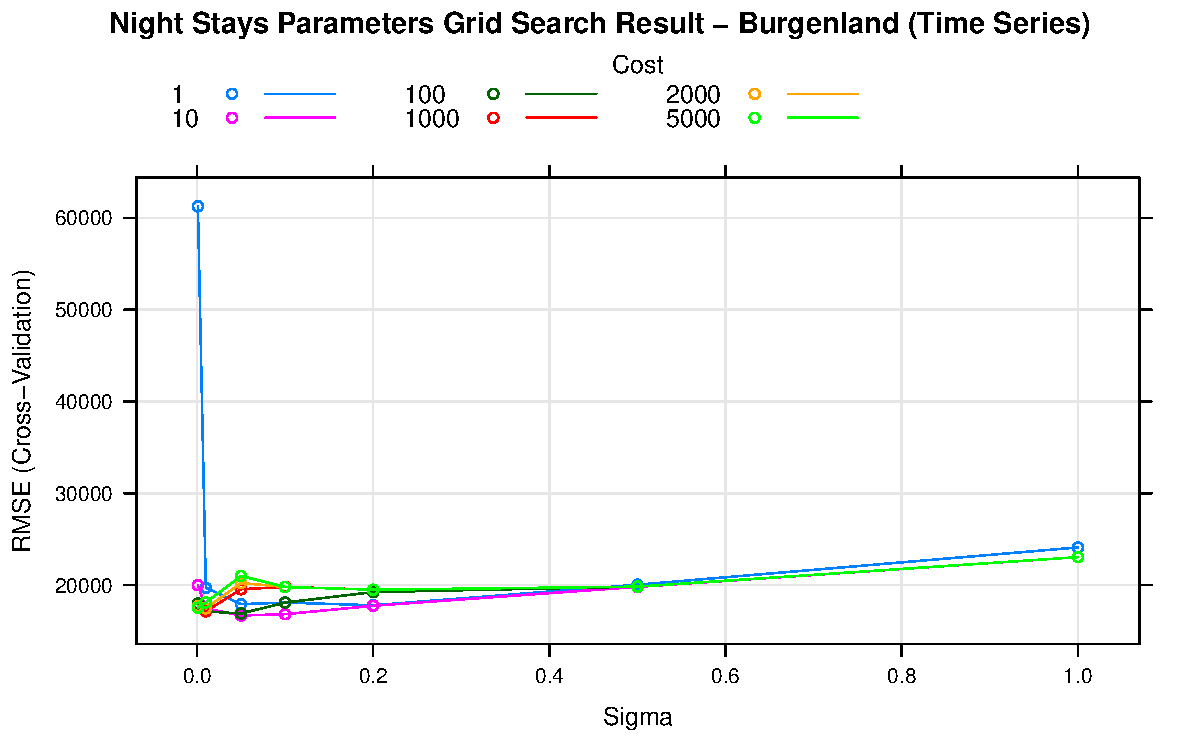
\includegraphics[width=\linewidth]{images/SVR/BurgenlandGrid.pdf}
    \caption{Training errors for parameters}
  \end{subfigure}
  \begin{subfigure}[b]{0.32\linewidth}
    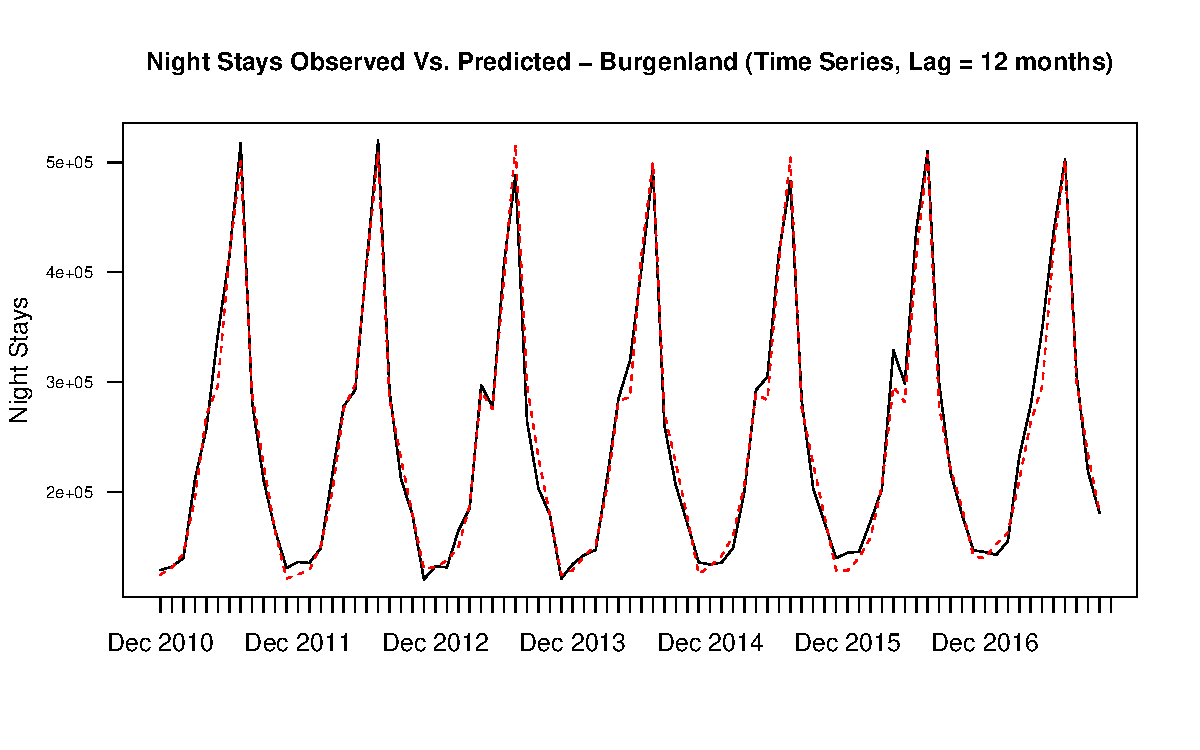
\includegraphics[width=\linewidth]{images/SVR/BurgenlandTimeSeries.pdf}
    \caption{Prediction Vs. Observation Fit}
  \end{subfigure}
  \begin{subfigure}[b]{0.32\linewidth}
    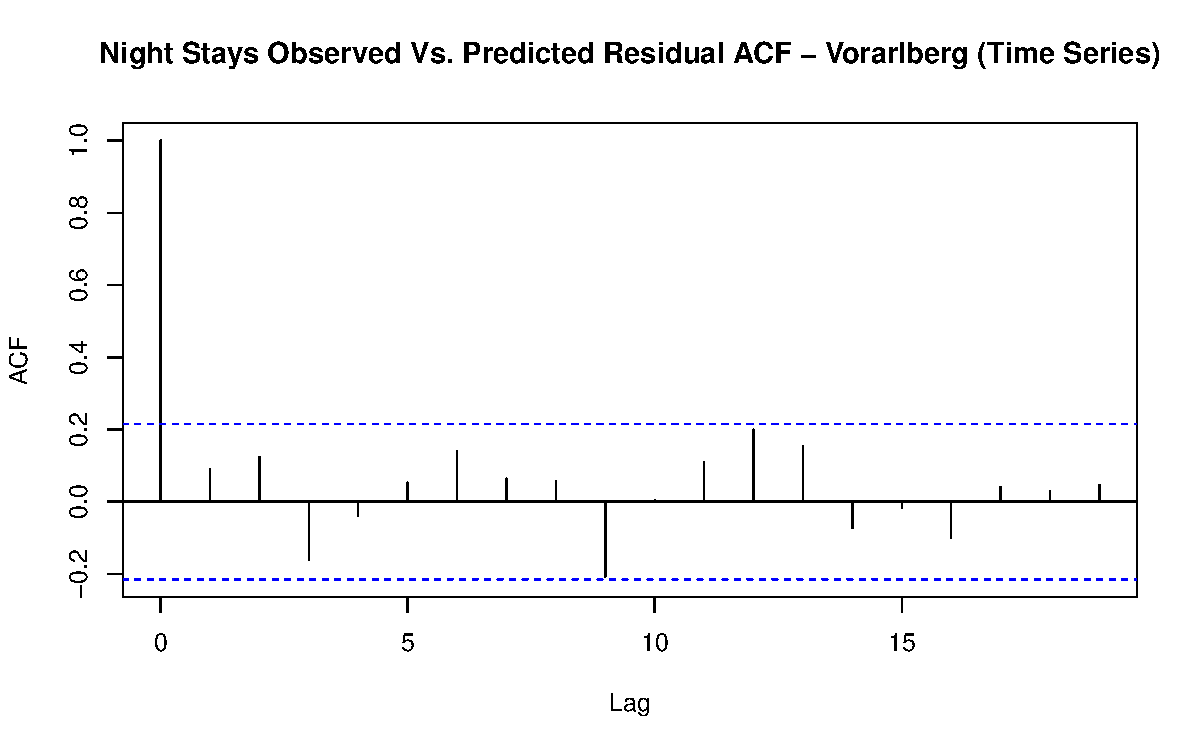
\includegraphics[width=\linewidth]{images/SVR/BurgenlandACF.pdf}
    \caption{Residual Autocorrelation}
  \end{subfigure}
  \caption{Burgenland Time Series Modelling}
  \label{fig:Time Series}
\end{figure}

\begin{longtable}[h!]
{!{\vrule width0.05cm}g!{\vrule width0.05cm}g!{\vrule width0.05cm}g!{\vrule width0.05cm}g!{\vrule width0.05cm}g!{\vrule width0.05cm}g!{\vrule width0.05cm}g!{\vrule width0.05cm}g!{\vrule width0.05cm}g!{\vrule width0.05cm}g!{\vrule width0.05cm}}
\specialrule{0.05cm}{.0cm}{.0cm}
\multicolumn{1}{!{\vrule width0.05cm}c!{\vrule width0.05cm}}
{\bfseries Province \par} & 
\multicolumn{1}{c!{\vrule width0.03cm}}{\bfseries Kernel \par} &
\multicolumn{1}{c!{\vrule width0.03cm}}{\bfseries RMSE Train \par} &
\multicolumn{1}{c!{\vrule width0.03cm}}{\bfseries RMSE Test\par} &
\multicolumn{1}{c!{\vrule width0.03cm}}{\bfseries R.Sq. Train \par} &
\multicolumn{1}{c!{\vrule width0.03cm}}{\bfseries R.Sq. Test \par} &
\multicolumn{1}{c!{\vrule width0.03cm}}{\bfseries Lag (m) \par}
\\ 
\specialrule{0.025cm}{.0cm}{.0cm}
\rowcolor{white}Burgenland & Radial Basis &	17361.51 &	160926.6 &	0.9864797 &	0.9848345 &	12\\
\specialrule{0.025cm}{.0cm}{.0cm}
\caption{Burgenland Final Model Result}
\label{tab:data_examp}
\end{longtable}
\noindent
The plot shows a tight fit against the observed night stays which is also validated by the residual ACF plot, which shows hardly any presence of significant autocorrelation in the residual. Subsequently the process is repeated for all the provinces using lags of six and 12 months while varying the kernels, followed by fine tuning their respective parameters with grid search. The results obtained are shown in the following. 
\begin{figure}[h!]
  \centering
  \begin{subfigure}[b]{0.32\linewidth}
    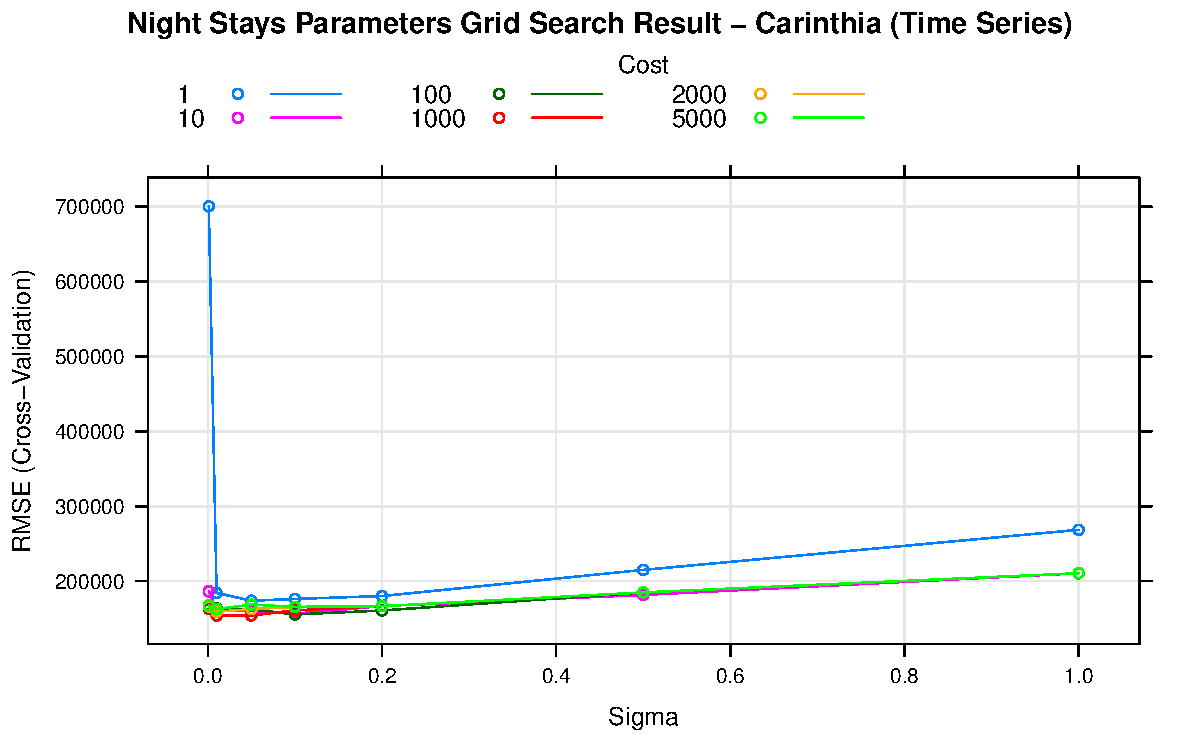
\includegraphics[width=\linewidth]{images/SVR/CarinthiaGrid.pdf}
    \caption{Training errors for parameters}
  \end{subfigure}
  \begin{subfigure}[b]{0.32\linewidth}
    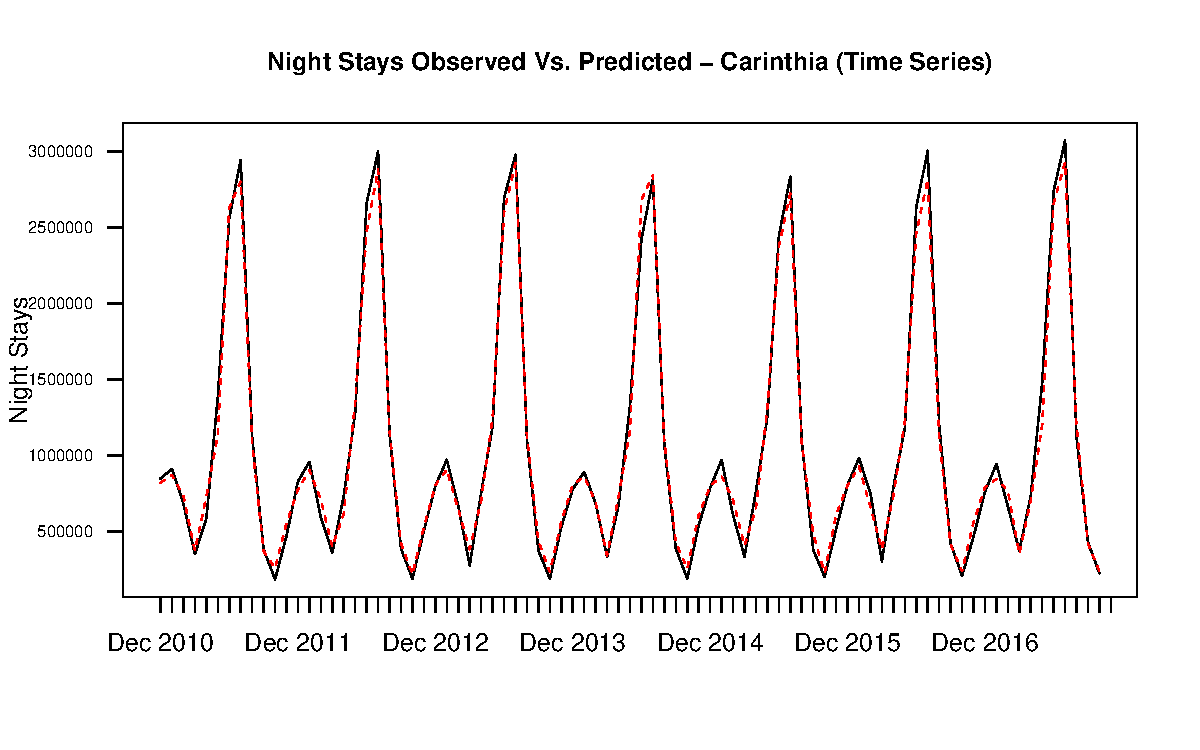
\includegraphics[width=\linewidth]{images/SVR/CarinthiaTimeSeries.pdf}
    \caption{Prediction Vs. Observation Fit}
  \end{subfigure}
  \begin{subfigure}[b]{0.32\linewidth}
    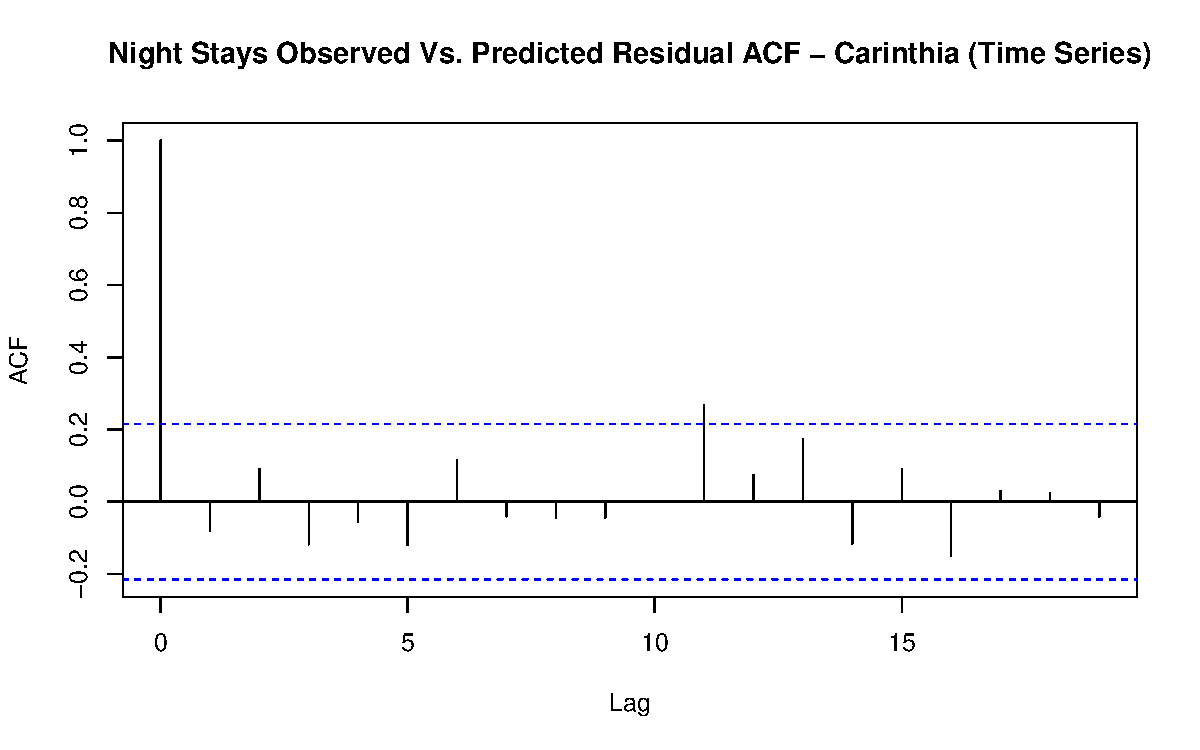
\includegraphics[width=\linewidth]{images/SVR/CarinthiaACF.pdf}
    \caption{Residual Autocorrelation}
  \end{subfigure}
  \caption{Carinthia Time Series Modelling using SVR}
  \label{fig:Time Series}
\end{figure}

\begin{longtable}[h!]
{!{\vrule width0.05cm}g!{\vrule width0.05cm}g!{\vrule width0.05cm}g!{\vrule width0.05cm}g!{\vrule width0.05cm}g!{\vrule width0.05cm}g!{\vrule width0.05cm}g!{\vrule width0.05cm}g!{\vrule width0.05cm}g!{\vrule width0.05cm}g!{\vrule width0.05cm}}
\specialrule{0.05cm}{.0cm}{.0cm}
\multicolumn{1}{!{\vrule width0.05cm}c!{\vrule width0.05cm}}
{\bfseries Province \par} & 
\multicolumn{1}{c!{\vrule width0.03cm}}{\bfseries Kernel \par} &
\multicolumn{1}{c!{\vrule width0.03cm}}{\bfseries RMSE Train \par} &
\multicolumn{1}{c!{\vrule width0.03cm}}{\bfseries RMSE Test\par} &
\multicolumn{1}{c!{\vrule width0.03cm}}{\bfseries R.Sq. Train \par} &
\multicolumn{1}{c!{\vrule width0.03cm}}{\bfseries R.Sq. Test \par} &
\multicolumn{1}{c!{\vrule width0.03cm}}{\bfseries Lag (m) \par}
\\ 
\specialrule{0.025cm}{.0cm}{.0cm}
\rowcolor{white}Carinthia & Radial Basis &	156698.50&84903.57&0.989495&0.9905645&12\\
\specialrule{0.025cm}{.0cm}{.0cm}
\caption{Carinthia Final Model Result}
\label{tab:data_examp}
\end{longtable}

\begin{figure}[H]
  \centering
  \begin{subfigure}[b]{0.32\linewidth}
    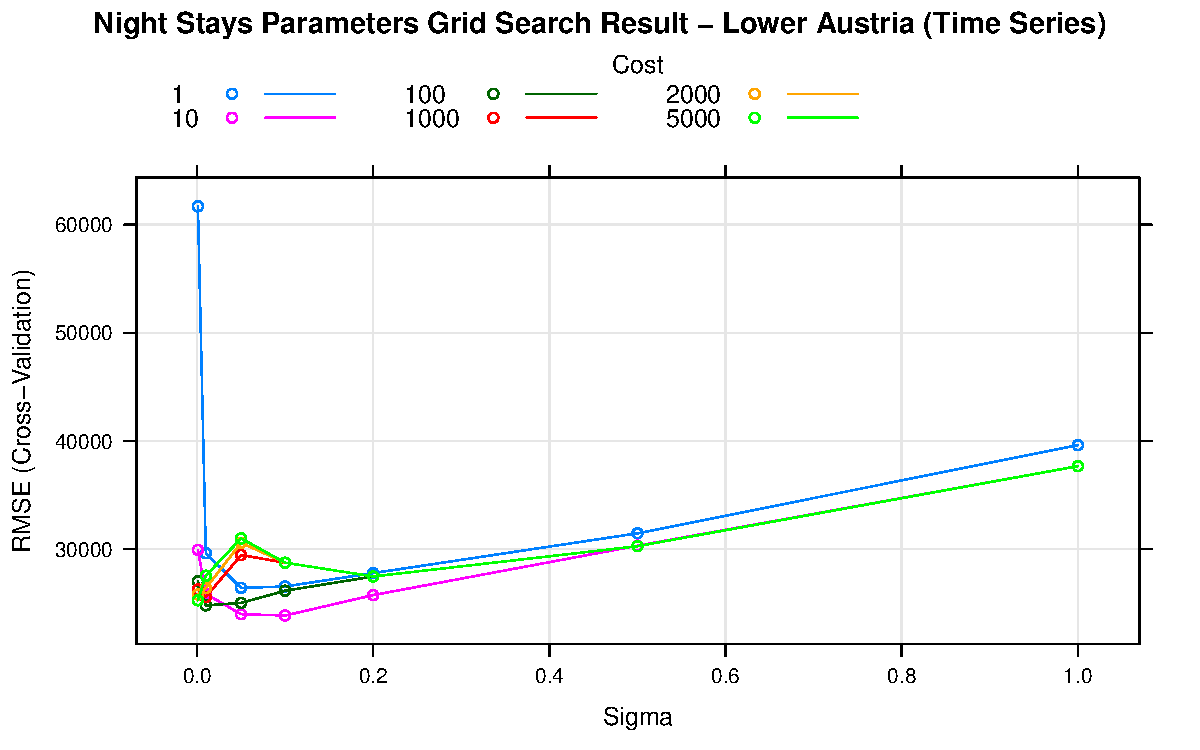
\includegraphics[width=\linewidth]{images/SVR/LowerAustriaGrid.pdf}
    \caption{Training errors for parameters}
  \end{subfigure}
  \begin{subfigure}[b]{0.32\linewidth}
    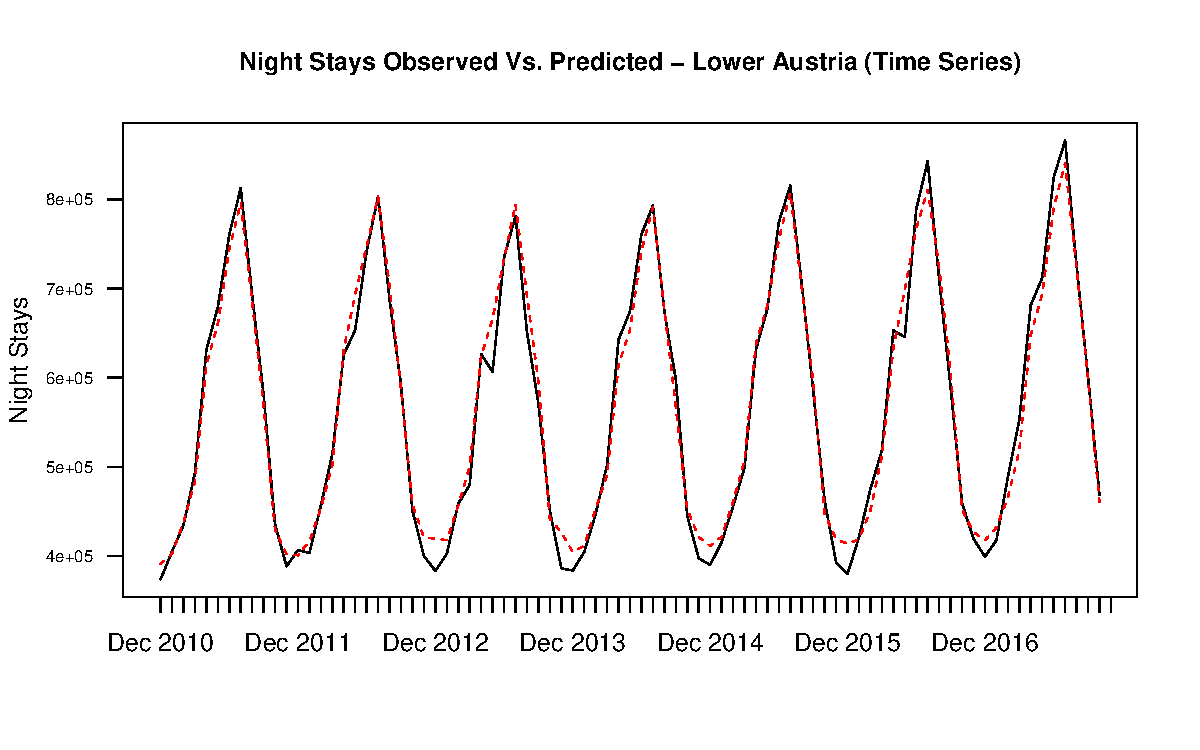
\includegraphics[width=\linewidth]{images/SVR/LowerAustriaTimeSeries.pdf}
    \caption{Prediction Vs. Observation Fit}
  \end{subfigure}
  \begin{subfigure}[b]{0.32\linewidth}
    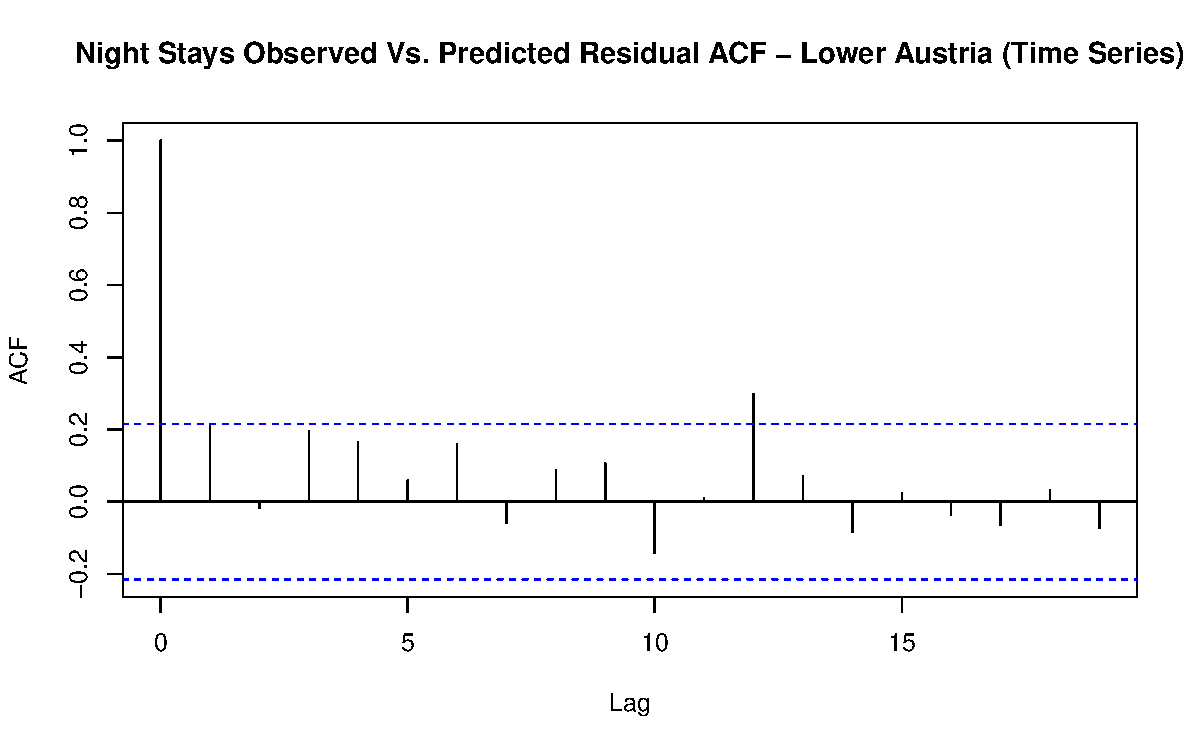
\includegraphics[width=\linewidth]{images/SVR/LowerAustriaACF.pdf}
    \caption{Residual Autocorrelation}
  \end{subfigure}
  \caption{Lower Austria Time Series Modelling using SVR}
  \label{fig:Time Series}
\end{figure}

\begin{longtable}[h!]
{!{\vrule width0.05cm}g!{\vrule width0.05cm}g!{\vrule width0.05cm}g!{\vrule width0.05cm}g!{\vrule width0.05cm}g!{\vrule width0.05cm}g!{\vrule width0.05cm}g!{\vrule width0.05cm}g!{\vrule width0.05cm}g!{\vrule width0.05cm}g!{\vrule width0.05cm}}
\specialrule{0.05cm}{.0cm}{.0cm}
\multicolumn{1}{!{\vrule width0.05cm}c!{\vrule width0.05cm}}
{\bfseries Province \par} & 
\multicolumn{1}{c!{\vrule width0.03cm}}{\bfseries Kernel \par} &
\multicolumn{1}{c!{\vrule width0.03cm}}{\bfseries RMSE Train \par} &
\multicolumn{1}{c!{\vrule width0.03cm}}{\bfseries RMSE Test\par} &
\multicolumn{1}{c!{\vrule width0.03cm}}{\bfseries R.Sq. Train \par} &
\multicolumn{1}{c!{\vrule width0.03cm}}{\bfseries R.Sq. Test \par} &
\multicolumn{1}{c!{\vrule width0.03cm}}{\bfseries Lag (m) \par}
\\ 
\specialrule{0.025cm}{.0cm}{.0cm}
\rowcolor{white}Lower Austria & Radial Basis &	23651.09&19964.21&0.9873452&0.9824075&12\\
\specialrule{0.025cm}{.0cm}{.0cm}
\caption{Lower Austria Final Model Result}
\label{tab:data_examp}
\end{longtable}

\begin{figure}[h!]
  \centering
  \begin{subfigure}[b]{0.32\linewidth}
    \includegraphics[width=\linewidth]{images/SVR/SalzburgGrid.pdf}
    \caption{Training errors for parameters}
  \end{subfigure}
  \begin{subfigure}[b]{0.32\linewidth}
    \includegraphics[width=\linewidth]{images/SVR/SalzburgTimeSeries.pdf}
    \caption{Prediction Vs. Observation Fit}
  \end{subfigure}
  \begin{subfigure}[b]{0.32\linewidth}
    \includegraphics[width=\linewidth]{images/SVR/SalzburgACF.pdf}
    \caption{Residual Autocorrelation}
  \end{subfigure}
  \caption{Salzburg Time Series Modelling using SVR}
  \label{fig:Time Series}
\end{figure}

\begin{longtable}[h!]
{!{\vrule width0.05cm}g!{\vrule width0.05cm}g!{\vrule width0.05cm}g!{\vrule width0.05cm}g!{\vrule width0.05cm}g!{\vrule width0.05cm}g!{\vrule width0.05cm}g!{\vrule width0.05cm}g!{\vrule width0.05cm}g!{\vrule width0.05cm}g!{\vrule width0.05cm}}
\specialrule{0.05cm}{.0cm}{.0cm}
\multicolumn{1}{!{\vrule width0.05cm}c!{\vrule width0.05cm}}
{\bfseries Province \par} & 
\multicolumn{1}{c!{\vrule width0.03cm}}{\bfseries Kernel \par} &
\multicolumn{1}{c!{\vrule width0.03cm}}{\bfseries RMSE Train \par} &
\multicolumn{1}{c!{\vrule width0.03cm}}{\bfseries RMSE Test\par} &
\multicolumn{1}{c!{\vrule width0.03cm}}{\bfseries R.Sq. Train \par} &
\multicolumn{1}{c!{\vrule width0.03cm}}{\bfseries R.Sq. Test \par} &
\multicolumn{1}{c!{\vrule width0.03cm}}{\bfseries Lag (m) \par}
\\ 
\specialrule{0.025cm}{.0cm}{.0cm}
\rowcolor{white}Lower Austria & Radial Basis &	160862.1&194640.2&0.9770268&0.9767925&12\\
\specialrule{0.025cm}{.0cm}{.0cm}
\caption{Salzburg Final Time Series Model Result}
\label{tab:data_examp}
\end{longtable}

\begin{figure}[H]
  \centering
  \begin{subfigure}[b]{0.32\linewidth}
    \includegraphics[width=\linewidth]{images/SVR/StyriaGrid.pdf}
    \caption{Training errors for parameters}
  \end{subfigure}
  \begin{subfigure}[b]{0.32\linewidth}
    \includegraphics[width=\linewidth]{images/SVR/StyriaTimeSeries.pdf}
    \caption{Prediction Vs. Observation Fit}
  \end{subfigure}
  \begin{subfigure}[b]{0.32\linewidth}
    \includegraphics[width=\linewidth]{images/SVR/StyriaACF.pdf}
    \caption{Residual Autocorrelation}
  \end{subfigure}
  \caption{Styria Time Series Modelling using SVR}
  \label{fig:Time Series}
\end{figure}

\begin{longtable}[h!]
{!{\vrule width0.05cm}g!{\vrule width0.05cm}g!{\vrule width0.05cm}g!{\vrule width0.05cm}g!{\vrule width0.05cm}g!{\vrule width0.05cm}g!{\vrule width0.05cm}g!{\vrule width0.05cm}g!{\vrule width0.05cm}g!{\vrule width0.05cm}g!{\vrule width0.05cm}}
\specialrule{0.05cm}{.0cm}{.0cm}
\multicolumn{1}{!{\vrule width0.05cm}c!{\vrule width0.05cm}}
{\bfseries Province \par} & 
\multicolumn{1}{c!{\vrule width0.03cm}}{\bfseries Kernel \par} &
\multicolumn{1}{c!{\vrule width0.03cm}}{\bfseries RMSE Train \par} &
\multicolumn{1}{c!{\vrule width0.03cm}}{\bfseries RMSE Test\par} &
\multicolumn{1}{c!{\vrule width0.03cm}}{\bfseries R.Sq. Train \par} &
\multicolumn{1}{c!{\vrule width0.03cm}}{\bfseries R.Sq. Test \par} &
\multicolumn{1}{c!{\vrule width0.03cm}}{\bfseries Lag (m) \par}
\\ 
\specialrule{0.025cm}{.0cm}{.0cm}
\rowcolor{white}Styria & Polynomial&49295.76&68445.17&0.9808474&0.9563754&12\\
\specialrule{0.025cm}{.0cm}{.0cm}
\caption{Styria Final Time Series SVR Model Result}
\label{tab:data_examp}
\end{longtable}

\begin{figure}[h!]
  \centering
  \begin{subfigure}[b]{0.32\linewidth}
    \includegraphics[width=\linewidth]{images/SVR/TyrolGrid.pdf}
    \caption{Training errors for parameters}
  \end{subfigure}
  \begin{subfigure}[b]{0.32\linewidth}
    \includegraphics[width=\linewidth]{images/SVR/TyrolTimeSeries.pdf}
    \caption{Prediction Vs. Observation Fit}
  \end{subfigure}
  \begin{subfigure}[b]{0.32\linewidth}
    \includegraphics[width=\linewidth]{images/SVR/TyrolACF.pdf}
    \caption{Residual Autocorrelation}
  \end{subfigure}
  \caption{Tyrol Time Series Modelling using SVR}
  \label{fig:Time Series}
\end{figure}

\begin{longtable}[h!]
{!{\vrule width0.05cm}g!{\vrule width0.05cm}g!{\vrule width0.05cm}g!{\vrule width0.05cm}g!{\vrule width0.05cm}g!{\vrule width0.05cm}g!{\vrule width0.05cm}g!{\vrule width0.05cm}g!{\vrule width0.05cm}g!{\vrule width0.05cm}g!{\vrule width0.05cm}}
\specialrule{0.05cm}{.0cm}{.0cm}
\multicolumn{1}{!{\vrule width0.05cm}c!{\vrule width0.05cm}}
{\bfseries Province \par} & 
\multicolumn{1}{c!{\vrule width0.03cm}}{\bfseries Kernel \par} &
\multicolumn{1}{c!{\vrule width0.03cm}}{\bfseries RMSE Train \par} &
\multicolumn{1}{c!{\vrule width0.03cm}}{\bfseries RMSE Test\par} &
\multicolumn{1}{c!{\vrule width0.03cm}}{\bfseries R.Sq. Train \par} &
\multicolumn{1}{c!{\vrule width0.03cm}}{\bfseries R.Sq. Test \par} &
\multicolumn{1}{c!{\vrule width0.03cm}}{\bfseries Lag (m) \par}
\\ 
\specialrule{0.025cm}{.0cm}{.0cm}
\rowcolor{white}Tyrol & Radial Basis &	308242.8&306728.4&0.9750711&0.9786044&12\\
\specialrule{0.025cm}{.0cm}{.0cm}
\caption{Tyrol Final Time Series SVR Model Result}
\label{tab:data_examp}
\end{longtable}

\begin{figure}[H]
  \centering
  \begin{subfigure}[b]{0.32\linewidth}
    \includegraphics[width=\linewidth]{images/SVR/UpperAustriaGrid.pdf}
    \caption{Training errors for parameters}
  \end{subfigure}
  \begin{subfigure}[b]{0.32\linewidth}
    \includegraphics[width=\linewidth]{images/SVR/UpperAustriaTimeSeries.pdf}
    \caption{Prediction Vs. Observation Fit}
  \end{subfigure}
  \begin{subfigure}[b]{0.32\linewidth}
    \includegraphics[width=\linewidth]{images/SVR/UpperAustriaACF.pdf}
    \caption{Residual Autocorrelation}
  \end{subfigure}
  \caption{Upper Austria Time Series Modelling using SVR}
  \label{fig:Time Series}
\end{figure}

\begin{longtable}[h!]
{!{\vrule width0.05cm}g!{\vrule width0.05cm}g!{\vrule width0.05cm}g!{\vrule width0.05cm}g!{\vrule width0.05cm}g!{\vrule width0.05cm}g!{\vrule width0.05cm}g!{\vrule width0.05cm}g!{\vrule width0.05cm}g!{\vrule width0.05cm}g!{\vrule width0.05cm}}
\specialrule{0.05cm}{.0cm}{.0cm}
\multicolumn{1}{!{\vrule width0.05cm}c!{\vrule width0.05cm}}
{\bfseries Province \par} & 
\multicolumn{1}{c!{\vrule width0.03cm}}{\bfseries Kernel \par} &
\multicolumn{1}{c!{\vrule width0.03cm}}{\bfseries RMSE Train \par} &
\multicolumn{1}{c!{\vrule width0.03cm}}{\bfseries RMSE Test\par} &
\multicolumn{1}{c!{\vrule width0.03cm}}{\bfseries R.Sq. Train \par} &
\multicolumn{1}{c!{\vrule width0.03cm}}{\bfseries R.Sq. Test \par} &
\multicolumn{1}{c!{\vrule width0.03cm}}{\bfseries Lag (m) \par}
\\ 
\specialrule{0.025cm}{.0cm}{.0cm}
\rowcolor{white}Upper Austria & Radial Basis &	40096.51&33886.15&0.9904772&0.9788871&12\\
\specialrule{0.025cm}{.0cm}{.0cm}
\caption{upper Austria Final Time Series SVR Model Result}
\label{tab:data_examp}
\end{longtable}

\begin{figure}[h!]
  \centering
  \begin{subfigure}[b]{0.32\linewidth}
    \includegraphics[width=\linewidth]{images/SVR/ViennaGrid.pdf}
    \caption{Training errors for parameters}
  \end{subfigure}
  \begin{subfigure}[b]{0.32\linewidth}
    \includegraphics[width=\linewidth]{images/SVR/ViennaTimeSeries.pdf}
    \caption{Prediction Vs. Observation Fit}
  \end{subfigure}
  \begin{subfigure}[b]{0.32\linewidth}
    \includegraphics[width=\linewidth]{images/SVR/ViennaACF.pdf}
    \caption{Residual Autocorrelation}
  \end{subfigure}
  \caption{Vienna Time Series Modelling using SVR}
  \label{fig:Time Series}
\end{figure}

\begin{longtable}[h!]
{!{\vrule width0.05cm}g!{\vrule width0.05cm}g!{\vrule width0.05cm}g!{\vrule width0.05cm}g!{\vrule width0.05cm}g!{\vrule width0.05cm}g!{\vrule width0.05cm}g!{\vrule width0.05cm}g!{\vrule width0.05cm}g!{\vrule width0.05cm}g!{\vrule width0.05cm}}
\specialrule{0.05cm}{.0cm}{.0cm}
\multicolumn{1}{!{\vrule width0.05cm}c!{\vrule width0.05cm}}
{\bfseries Province \par} & 
\multicolumn{1}{c!{\vrule width0.03cm}}{\bfseries Kernel \par} &
\multicolumn{1}{c!{\vrule width0.03cm}}{\bfseries RMSE Train \par} &
\multicolumn{1}{c!{\vrule width0.03cm}}{\bfseries RMSE Test\par} &
\multicolumn{1}{c!{\vrule width0.03cm}}{\bfseries R.Sq. Train \par} &
\multicolumn{1}{c!{\vrule width0.03cm}}{\bfseries R.Sq. Test \par} &
\multicolumn{1}{c!{\vrule width0.03cm}}{\bfseries Lag (m) \par}
\\ 
\specialrule{0.025cm}{.0cm}{.0cm}
\rowcolor{white}Vienna & Polynomial&39872.73&68355.33&0.9703751&0.932065&12\\
\specialrule{0.025cm}{.0cm}{.0cm}
\caption{Vienna Final Time Series SVR Model Result}
\label{tab:data_examp}
\end{longtable}

\begin{figure}[H]
  \centering
  \begin{subfigure}[b]{0.32\linewidth}
    \includegraphics[width=\linewidth]{images/SVR/VorarlbergGrid.pdf}
    \caption{Training errors for parameters}
  \end{subfigure}
  \begin{subfigure}[b]{0.32\linewidth}
    \includegraphics[width=\linewidth]{images/SVR/VorarlbergTimeSeries.pdf}
    \caption{Prediction Vs. Observation Fit}
  \end{subfigure}
  \begin{subfigure}[b]{0.32\linewidth}
    \includegraphics[width=\linewidth]{images/SVR/VorarlbergACF.pdf}
    \caption{Residual Autocorrelation}
  \end{subfigure}
  \caption{Vorarlberg Time Series Modelling using SVR}
  \label{fig:Time Series}
\end{figure}

\begin{longtable}[h!]
{!{\vrule width0.05cm}g!{\vrule width0.05cm}g!{\vrule width0.05cm}g!{\vrule width0.05cm}g!{\vrule width0.05cm}g!{\vrule width0.05cm}g!{\vrule width0.05cm}g!{\vrule width0.05cm}g!{\vrule width0.05cm}g!{\vrule width0.05cm}g!{\vrule width0.05cm}}
\specialrule{0.05cm}{.0cm}{.0cm}
\multicolumn{1}{!{\vrule width0.05cm}c!{\vrule width0.05cm}}
{\bfseries Province \par} & 
\multicolumn{1}{c!{\vrule width0.03cm}}{\bfseries Kernel \par} &
\multicolumn{1}{c!{\vrule width0.03cm}}{\bfseries RMSE Train \par} &
\multicolumn{1}{c!{\vrule width0.03cm}}{\bfseries RMSE Test\par} &
\multicolumn{1}{c!{\vrule width0.03cm}}{\bfseries R.Sq. Train \par} &
\multicolumn{1}{c!{\vrule width0.03cm}}{\bfseries R.Sq. Test \par} &
\multicolumn{1}{c!{\vrule width0.03cm}}{\bfseries Lag (m) \par}
\\ 
\specialrule{0.025cm}{.0cm}{.0cm}
\rowcolor{white}Vorarlberg & Radial Basis&70599.05&65505.49&0.9645311&0.9714037&12\\
\specialrule{0.025cm}{.0cm}{.0cm}
\caption{Vorarlberg Final Time Series SVR Model Result}
\label{tab:data_examp}
\end{longtable}
\noindent
Finally all the results are compiled in the table below. The result shows a high test R-square for all the provinces using the lag of 12 month rather than six. In most of the cases the RBF Kernel returns the best fit except in case of Vienna and Styria where the Polynomial kernel with degrees 2 out performed the RBF kernels. This is interesting since for the case of Vienna there seems to be multiple annual peaks of night stays compared to other provinces.  

\begin{longtable}[h!]
{!{\vrule width0.05cm}g!{\vrule width0.05cm}g!{\vrule width0.05cm}g!{\vrule width0.05cm}g!{\vrule width0.05cm}g!{\vrule width0.05cm}g!{\vrule width0.05cm}g!{\vrule width0.05cm}g!{\vrule width0.05cm}g!{\vrule width0.05cm}g!{\vrule width0.05cm}}
\specialrule{0.05cm}{.0cm}{.0cm}
\multicolumn{1}{!{\vrule width0.05cm}c!{\vrule width0.05cm}}
{\bfseries Province \par} & 
\multicolumn{1}{c!{\vrule width0.03cm}}{\bfseries Kernel \par} &
\multicolumn{1}{c!{\vrule width0.03cm}}{\bfseries RMSE Train \par} &
\multicolumn{1}{c!{\vrule width0.03cm}}{\bfseries RMSE Test\par} &
\multicolumn{1}{c!{\vrule width0.03cm}}{\bfseries R.Sq. Train \par} &
\multicolumn{1}{c!{\vrule width0.03cm}}{\bfseries R.Sq. Test \par} &
\multicolumn{1}{c!{\vrule width0.03cm}}{\bfseries Lag (m) \par}
\\ 
\specialrule{0.05cm}{.0cm}{.0cm} 
Burgenland & Radial Basis &	25472.08&170770.2&0.9679858&0.9578215&6
 \\ \specialrule{0.025cm}{.0cm}{.0cm}
\rowcolor{white}Burgenland & Radial Basis &	17361.51&14351.83
&0.9864797&\cellcolor[rgb]{ .996,  .8,  .494}0.9851352&12
\\
\specialrule{0.05cm}{.0cm}{.0cm} 
Carinthia & Radial Basis &	160763&151872.4	&0.9750809&0.9882232&6
 \\ \specialrule{0.025cm}{.0cm}{.0cm}
\rowcolor{white}Carinthia & Radial Basis &	156698.50&84903.57&0.989495&\cellcolor[rgb]{ .996,  .8,  .494}0.9905645&12
\\
\specialrule{0.05cm}{.0cm}{.0cm} 
Lower Austria & Radial Basis &	40460.03&33884.31&0.965073&0.9534268&6
 \\ \specialrule{0.025cm}{.0cm}{.0cm}
\rowcolor{white}Lower Austria & Radial Basis &	23651.09&19964.21&0.9873452&\cellcolor[rgb]{ .996,  .8,  .494}0.9824075&12
\\
\specialrule{0.025cm}{.0cm}{.0cm}
Salzburg & Radial Basis &	212233.70&318559&0.9601843&0.9359245&6
 \\ \specialrule{0.025cm}{.0cm}{.0cm}
\rowcolor{white}Salzburg & Radial Basis &	160862.1&194640.2&0.9770268&\cellcolor[rgb]{ .996,  .8,  .494}0.9767925&12
\\
\specialrule{0.025cm}{.0cm}{.0cm}
Styria & Radial Basis &	45190.7&90598.99&0.9834137&0.9470502&12
 \\ \specialrule{0.025cm}{.0cm}{.0cm}
\rowcolor{white}Styria & Polynomial&49295.76&68445.17&0.9808474&\cellcolor[rgb]{ .996,  .8,  .494}0.9563754&12
\\
\specialrule{0.025cm}{.0cm}{.0cm}
Tyrol & Radial Basis &	416286.5&451811.5&0.9553336&0.9579362&6
 \\ \specialrule{0.025cm}{.0cm}{.0cm}
\rowcolor{white}Tyrol & Radial Basis &	308242.8&306728.4&0.9750711&\cellcolor[rgb]{ .996,  .8,  .494}0.9786044&12
\\
\specialrule{0.025cm}{.0cm}{.0cm}
Upper Austria & Radial Basis &	67516.86&69164.82&0.9749186&0.9076577&6
 \\ \specialrule{0.025cm}{.0cm}{.0cm}
\rowcolor{white}Upper Austria & Radial Basis &	40096.51&33886.15&0.9904772&\cellcolor[rgb]{ .996,  .8,  .494}0.9788871&12
\\
\specialrule{0.025cm}{.0cm}{.0cm}
Vienna & Radial Basis &	34655.17&376822.9&0.9779828&0.2135794&12
 \\ \specialrule{0.025cm}{.0cm}{.0cm}
\rowcolor{white}Vienna & Polynomial&39872.73&68355.33&0.9703751&\cellcolor[rgb]{ .996,  .8,  .494}0.932065&12
\\
\specialrule{0.025cm}{.0cm}{.0cm}
Vorarlberg & Radial Basis &	88921.27&100286.6&0.9444394&0.9536337&6
 \\ \specialrule{0.025cm}{.0cm}{.0cm}
\rowcolor{white}Vorarlberg & Radial Basis&70599.05&65505.49&0.9645311&\cellcolor[rgb]{ .996,  .8,  .494}0.9714037&12
\\
\specialrule{0.025cm}{.0cm}{.0cm}
\caption{Time Series Modelling Using Different Lags in Support Vector Regression (SVR)}
\label{tab:data_examp}
\end{longtable}
\noindent
\subsubsection{Results - Space-Time SVR Model}
The time series model discussed in the previous section fitted the observed data considerably well as was found from the RMSE and r-square values. Although no significant spatial autocorrelation was indicated in the data, which may be due to estimation using too few data points, a Space-Time Modelling of the data is attempted to verify if there would be any improvements in result. For implementing the space-time algorithm first the spatial weight matrix is estimated. Two types of weight matrix is tested to find the suitable weight matrix. One is the spatial adjacency weight matrix which is calculated on the basis of provinces sharing boundary with each other. Subsequently a SVR model is fitted using this weight matrix for Burgenland. The result shows that the RMSE values for the test increases for the test, though the model fits well on the training with high R-Squares for the training model.

\begin{longtable}[h!]
{!{\vrule width0.05cm}g!{\vrule width0.05cm}g!{\vrule width0.05cm}g!{\vrule width0.05cm}g!{\vrule width0.05cm}g!{\vrule width0.05cm}g!{\vrule width0.05cm}}
\specialrule{0.05cm}{.0cm}{.0cm}
\multicolumn{1}{!{\vrule width0.05cm}c!{\vrule width0.05cm}}
{\bfseries Weight Matrix \par} & 
\multicolumn{1}{c!{\vrule width0.03cm}}{\bfseries RMSE Train \par} &
\multicolumn{1}{c!{\vrule width0.03cm}}{\bfseries RMSE Test \par} &
\multicolumn{1}{c!{\vrule width0.03cm}}{\bfseries R-Sq Train \par} &
\multicolumn{1}{c!{\vrule width0.03cm}}{\bfseries R-Sq Test \par}&
\multicolumn{1}{c!{\vrule width0.03cm}}{\bfseries Lag \par}
\\ 
\specialrule{0.025cm}{.0cm}{.0cm}
\rowcolor{white}W – Adjacency &	8491.55 &	21580.54 &	0.9287 &	0.7237 &	2\\
\specialrule{0.025cm}{.0cm}{.0cm}
\rowcolor{lightgray}W – Adjacency &	5728.35 &	20252.70 &	0.9673 &	0.7730 &	3

\\
\specialrule{0.025cm}{.0cm}{.0cm}
\rowcolor{white}W – Adjacency &	3511.3470 &	17840.2300 &	0.9877 &	0.8192&	4
\\
\specialrule{0.025cm}{.0cm}{.0cm}
\caption{Space-Time Series SVR Model Result Using Adjacency Weight Matrix}
\label{tab:data_examp}
\end{longtable}
\noindent
Now the test is repeated using a second spatial weight matrix which is created using the length of the shared border of each neighboring provinces and row normalized. The parameters are retained from the previous model for comparison. 
\begin{longtable}[h!]
{!{\vrule width0.05cm}g!{\vrule width0.05cm}g!{\vrule width0.05cm}g!{\vrule width0.05cm}g!{\vrule width0.05cm}g!{\vrule width0.05cm}g!{\vrule width0.05cm}}
\specialrule{0.05cm}{.0cm}{.0cm}
\multicolumn{1}{!{\vrule width0.05cm}c!{\vrule width0.05cm}}
{\bfseries Weight Matrix \par} & 
\multicolumn{1}{c!{\vrule width0.03cm}}{\bfseries RMSE Train \par} &
\multicolumn{1}{c!{\vrule width0.03cm}}{\bfseries RMSE Test \par} &
\multicolumn{1}{c!{\vrule width0.03cm}}{\bfseries R-Sq Train \par} &
\multicolumn{1}{c!{\vrule width0.03cm}}{\bfseries R-Sq Test \par}&
\multicolumn{1}{c!{\vrule width0.03cm}}{\bfseries Lag \par}
\\ 
\specialrule{0.025cm}{.0cm}{.0cm}
\rowcolor{white}W – boundary &	5481.2710 &	13408.2200 &	0.9699 &	0.8499 &	2
\\
\specialrule{0.025cm}{.0cm}{.0cm}
\rowcolor{lightgray}W – boundary &	3547.4340 &	11452.3700 &	0.9874 &	0.9144 &	3
\\
\specialrule{0.025cm}{.0cm}{.0cm}
\rowcolor{white}W – boundary &	3028.29 &	11849.80 &	0.9908 &	0.9196 &	4
\\
\specialrule{0.025cm}{.0cm}{.0cm}
\caption{Space-Time Series SVR Model Result Using Length of Boundary Shared Weight Matrix}
\label{tab:data_examp}
\end{longtable}
\noindent
The result shows that there is slight improvement in both the training as well as the test model. The residual autocorelation plot of both the type of weight matrices plot also shows there has been improvement with lesser ACF present in the residual for the length share matrix. Henceforth the shared length boundary spatial weight matrix is used to embed the data. Subsequently the data set is split into test and train, fitted to a space-time SVR model while fine tuning the model by varying the different general parameters along with the kernels of radial basis and polynomial function and the related kernel specific parameter. The result is measured using the RMSE values and the R square values and is summarized as follows:  
\begin{longtable}[h!]
{!{\vrule width0.05cm}g!{\vrule width0.05cm}g!{\vrule width0.05cm}g!{\vrule width0.05cm}g!{\vrule width0.05cm}g!{\vrule width0.05cm}g!{\vrule width0.05cm}}
\specialrule{0.05cm}{.0cm}{.0cm}
\multicolumn{1}{!{\vrule width0.05cm}c!{\vrule width0.05cm}}
{\bfseries Provinces \par} & 
\multicolumn{1}{c!{\vrule width0.03cm}}{\bfseries Train RMSE	\par} &
\multicolumn{1}{c!{\vrule width0.03cm}}{\bfseries Test RMSE	  \par} &
\multicolumn{1}{c!{\vrule width0.03cm}}{\bfseries Train R Square	 \par} &
\multicolumn{1}{c!{\vrule width0.03cm}}{\bfseries Test R Square	 \par}&
\multicolumn{1}{c!{\vrule width0.03cm}}{\bfseries Kernel \par}
\\ 
\specialrule{0.025cm}{.0cm}{.0cm}
\rowcolor{white}Burgenland &	26246.46 &	34420.62 &	0.9688 &0.9248 &	Polynomial
\\
\specialrule{0.025cm}{.0cm}{.0cm}
\rowcolor{lightgray}Carinthia &	88727.83 &	168847.00 &	0.9964 &0.9644 &Radial Basis
\\
\specialrule{0.025cm}{.0cm}{.0cm}
\rowcolor{white}Lower Austria &	10982.09 &	26954.60 &	0.9974	& 0.9657 &	Radial Basis
\\
\specialrule{0.025cm}{.0cm}{.0cm}
\rowcolor{lightgray} Salzburg &	107766.90 &	281138.70 &	0.9896	& 0.9465 &	Radial Basis
\\
\specialrule{0.025cm}{.0cm}{.0cm}
\rowcolor{white} Styria &	41728.64 &	73149.92 &	0.9864	& 0.9558 &	Radial Basis
\\
\specialrule{0.025cm}{.0cm}{.0cm}
\rowcolor{lightgray} Tyrol &	267445.10 &	381466.00 &	0.9815	& 0.9645 &	Radial Basis
\\
\specialrule{0.025cm}{.0cm}{.0cm}
\rowcolor{white}Upper Austria &	58961.09 &	78319.51 &	0.9819	& 0.9359 &	Radial Basis
\\
\specialrule{0.025cm}{.0cm}{.0cm}
\rowcolor{lightgray} Vienna &	32918.21 &	98301.73 &	0.9797	& 0.8970 &	Polynomial
\\
\specialrule{0.025cm}{.0cm}{.0cm}
\rowcolor{white}Vorarlberg &	41003.13 &	77126.05 &	0.9880	& 0.9592 &	Radial Basis
\\
\specialrule{0.025cm}{.0cm}{.0cm}
\caption{Space-Time Series Final SVR Model Result Using Length of Boundary Shared Weight Matrix}
\label{tab:data_examp}
\end{longtable}
\noindent
Among the various kernels the polynomial and Gaussian RBF kernels returned the best fit. The polynomial kernels performed better for data with irregular pattern of multiple peaks and troughs where RBF kernels were unable to capture the deviation especially for Burgenland and Vienna. In the rest of the instances RBF outperformed polynomial kernels in terms of both fit and training time. The training time for the polynomial kernels model were significantly higher than a SVR model using a Radial basis kernel.

\begin{figure}[H]
  \centering
  \begin{subfigure}[b]{0.32\linewidth}
    \includegraphics[width=\linewidth]{images/SVR/BurgenlandSpaceTimeSVR.pdf}
    \caption{Burgenland}
  \end{subfigure}
  \begin{subfigure}[b]{0.32\linewidth}
    \includegraphics[width=\linewidth]{images/SVR/CarinthiaSpaceTimeSVR.pdf}
    \caption{Carinthia}
  \end{subfigure}
  \begin{subfigure}[b]{0.32\linewidth}
    \includegraphics[width=\linewidth]{images/SVR/LowerAustriaSpaceTimeSVR.pdf}
    \caption{LowerAustria}
  \end{subfigure}
  \begin{subfigure}[b]{0.32\linewidth}
    \includegraphics[width=\linewidth]{images/SVR/SalzburgSpaceTimeSVR.pdf}
    \caption{Salzburg}
  \end{subfigure}
  \begin{subfigure}[b]{0.32\linewidth}
    \includegraphics[width=\linewidth]{images/SVR/StyriaSpaceTimeSVR.pdf}
    \caption{Styria}
  \end{subfigure}
  \begin{subfigure}[b]{0.32\linewidth}
    \includegraphics[width=\linewidth]{images/SVR/TyrolSpaceTimeSVR.pdf}
    \caption{Tyrol}
  \end{subfigure}
  \begin{subfigure}[b]{0.32\linewidth}
    \includegraphics[width=\linewidth]{images/SVR/UpperAustriaSpaceTimeSVR.pdf}
    \caption{Upper Austria}
  \end{subfigure}
  \begin{subfigure}[b]{0.32\linewidth}
    \includegraphics[width=\linewidth]{images/SVR/ViennaSpaceTimeSVR.pdf}
    \caption{Vienna}
  \end{subfigure}
  \begin{subfigure}[b]{0.32\linewidth}
    \includegraphics[width=\linewidth]{images/SVR/VorarlbergSpaceTimeSVR.pdf}
    \caption{Vorarlberg}
  \end{subfigure}
  \caption{Observed vs Predicted Night Stays values for the SVR Space-Time model}
  \label{fig:Time Series}
\end{figure}

\subsubsection{Discussion}
Comparison of the SVR model output from the time series versus the space-time series models clearly indicate that the time series model performs significantly better than the space-time model. Hence it could be concluded that there is not much spatial component in the data, as was indicated by Moran's I.
\begin{longtable}[h!]
{!{\vrule width0.05cm}g!{\vrule width0.05cm}g!{\vrule width0.05cm}g!{\vrule width0.05cm}g!{\vrule width0.05cm}g!{\vrule width0.05cm}}
\specialrule{0.05cm}{.0cm}{.0cm}
\multicolumn{1}{!{\vrule width0.05cm}c!{\vrule width0.05cm}}
{\bfseries Provinces \par} & 
\multicolumn{1}{c!{\vrule width0.03cm}}{\bfseries Tm Test RMSE \par} &
\multicolumn{1}{c!{\vrule width0.03cm}}{\bfseries Sp-Tm Test RMSE 	  \par} &
\multicolumn{1}{c!{\vrule width0.03cm}}{\bfseries Tm Test R-Sq	 \par} &
\multicolumn{1}{c!{\vrule width0.03cm}}{\bfseries Sp-Tm Test R-Sq \par}
\\ 
\specialrule{0.025cm}{.0cm}{.0cm}
\rowcolor{white}Burgenland &	14352 & 34421 & 0.9851 & 0.9248
\\
\specialrule{0.025cm}{.0cm}{.0cm}
\rowcolor{lightgray}Carinthia &	84904 &	168847 & 0.9906 & 0.9644
\\
\specialrule{0.025cm}{.0cm}{.0cm}
\rowcolor{white}Lower Austria &	19964 &	26955 &	0.9824 & 0.9657
\\
\specialrule{0.025cm}{.0cm}{.0cm}
\rowcolor{lightgray} Salzburg &	194640 & 281139 & 0.9768 & 0.9465
\\
\specialrule{0.025cm}{.0cm}{.0cm}
\rowcolor{white} Styria &	68445 &	73150 &	0.9564 & 0.9558

\\
\specialrule{0.025cm}{.0cm}{.0cm}
\rowcolor{lightgray} Tyrol & 306728 & 381466 & 0.9786 &	0.9645
\\
\specialrule{0.025cm}{.0cm}{.0cm}
\rowcolor{white}Upper Austria &	33886 &	78320 &	0.9789 & 0.9359
\\
\specialrule{0.025cm}{.0cm}{.0cm}
\rowcolor{lightgray} Vienna &	68355 & 98302 & 0.9321 & 0.8970
\\
\specialrule{0.025cm}{.0cm}{.0cm}
\rowcolor{white}Vorarlberg & 65505 & 77126 & 0.9714 & 0.9592
\\
\specialrule{0.025cm}{.0cm}{.0cm}
\caption{Time Series Vs. Space-Time Series SVR Model Comparison of Night Stays}
\label{tab:data_examp}
\end{longtable}
\noindent
Another interesting output of the SVR model is the number of support vectors used by the model to train the data. The table below shows that the maximum number of support vectors used was 47 percent of the train data for the provinces of Tyrol and Vienna, while the least was for the province of Carinthia which was only around 19 percent of the data, and fitting the data considerably well with 0.989 r square. This is one of the strength of Support Vector Regression that it only requires a fraction of the data to fit a model reasonably well which prevents the model from over fitting.  
\begin{longtable}[h!]
{!{\vrule width0.05cm}g!{\vrule width0.05cm}g!{\vrule width0.05cm}g!{\vrule width0.05cm}g!{\vrule width0.05cm}g!{\vrule width0.05cm}}
\specialrule{0.05cm}{.0cm}{.0cm}
\multicolumn{1}{!{\vrule width0.05cm}c!{\vrule width0.05cm}}
{\bfseries Provinces \par} & 
\multicolumn{1}{c!{\vrule width0.03cm}}{\bfseries No. of Support Vectors \par} &
\multicolumn{1}{c!{\vrule width0.03cm}}{\bfseries Percentage of Data \par} &
\multicolumn{1}{c!{\vrule width0.03cm}}{\bfseries Kernel	 \par} &
\multicolumn{1}{c!{\vrule width0.03cm}}{\bfseries Training Time(sec) \par}
\\ 
\specialrule{0.025cm}{.0cm}{.0cm}
\rowcolor{white}Burgenland & 120 &	27.65\% & Polynomial & 123.54
\\
\specialrule{0.025cm}{.0cm}{.0cm}
\rowcolor{lightgray}Carinthia &	81 & 18.66\% & Radial Basis & 2.92
\\
\specialrule{0.025cm}{.0cm}{.0cm}
\rowcolor{white}Lower Austria &	93 & 21.43\% &	Radial Basis & 1.82
\\
\specialrule{0.025cm}{.0cm}{.0cm}
\rowcolor{lightgray} Salzburg &	181 & 41.71\% &	Radial Basis & 0.49
\\
\specialrule{0.025cm}{.0cm}{.0cm}
\rowcolor{white} Styria & 175 & 40.32\% &	Polynomial & 1.14 
\\
\specialrule{0.025cm}{.0cm}{.0cm}
\rowcolor{lightgray} Tyrol & 204 & 47.00\% & Radial Basis &	1.12
\\
\specialrule{0.025cm}{.0cm}{.0cm}
\rowcolor{white}Upper Austria &	89 & 20.51\% & Radial Basis & 1.42
\\
\specialrule{0.025cm}{.0cm}{.0cm}
\rowcolor{lightgray} Vienna & 204 &	47.00\% & Polynomial & 207.95
\\
\specialrule{0.025cm}{.0cm}{.0cm}
\rowcolor{white}Vorarlberg & 193 & 44.47\% & Radial Basis & 0.67
\\
\specialrule{0.025cm}{.0cm}{.0cm}
\caption{No. of Support Vectors and Kernel Training Time for SVR Models}
\label{tab:data_examp}
\end{longtable}
\noindent
Finally the n-step method is used to predict tourist night stays from 2011, January to 2017, November using only 12 months of data of the year 2010 for each of the provinces. The predictions are then compared with actual data from during the same period
\begin{longtable}[h!]
{!{\vrule width0.05cm}g!{\vrule width0.05cm}g!{\vrule width0.05cm}g!{\vrule width0.05cm}}
\specialrule{0.05cm}{.0cm}{.0cm}
\multicolumn{1}{!{\vrule width0.05cm}c!{\vrule width0.05cm}}{\bfseries Provinces \par} & 
\multicolumn{1}{c!{\vrule width0.03cm}}{\bfseries RMSE \par} &
\multicolumn{1}{c!{\vrule width0.03cm}}{\bfseries R-Square \par}  
\\ 
\specialrule{0.025cm}{.0cm}{.0cm}
\rowcolor{white}Burgenland & 26856 & 0.959427 
\\
\specialrule{0.025cm}{.0cm}{.0cm}
\rowcolor{lightgray}Carinthia &	417777 & 0.773698  
\\
\specialrule{0.025cm}{.0cm}{.0cm}
\rowcolor{white}Lower Austria &	75217 & 0.827141  
\\
\specialrule{0.025cm}{.0cm}{.0cm}
\rowcolor{lightgray} Salzburg &	219775 & 0.974860 
\\
\specialrule{0.025cm}{.0cm}{.0cm}
\rowcolor{white} Styria & 138864 & 0.895087 
\\
\specialrule{0.025cm}{.0cm}{.0cm}
\rowcolor{lightgray} Tyrol & 410525 & 0.971745  
\\
\specialrule{0.025cm}{.0cm}{.0cm}
\rowcolor{white}Upper Austria &	92469 & 0.943894 
\\
\specialrule{0.025cm}{.0cm}{.0cm}
\rowcolor{lightgray} Vienna & 220018 & 0.581188   
\\
\specialrule{0.025cm}{.0cm}{.0cm}
\rowcolor{white}Vorarlberg & 113202 & 0.938909  
\\
\specialrule{0.025cm}{.0cm}{.0cm}
\caption{Comparison of SVR N-Step Predicted Result to Observed Night Stays, 2011 – 2017}
\label{tab:data_examp}
\end{longtable}
\noindent
The best prediction is obtained for Salzburg with a r-square of 0.9748, whereas the worst is estimated for Vienna with a r-square of 0.5811.   

\begin{figure}[H]
  \centering
  \begin{subfigure}[b]{0.32\linewidth}
    \includegraphics[width=\linewidth]{images/SVR/BurgenlandNstepSVR.pdf}
    \caption{Burgenland}
  \end{subfigure}
  \begin{subfigure}[b]{0.32\linewidth}
    \includegraphics[width=\linewidth]{images/SVR/CarinthiaNstepSVR.pdf}
    \caption{Carinthia}
  \end{subfigure}
  \begin{subfigure}[b]{0.32\linewidth}
    \includegraphics[width=\linewidth]{images/SVR/LowerAustriaNstepSVR.pdf}
    \caption{LowerAustria}
  \end{subfigure}
  \begin{subfigure}[b]{0.32\linewidth}
    \includegraphics[width=\linewidth]{images/SVR/SalzburgNstepSVR.pdf}
    \caption{Salzburg}
  \end{subfigure}
  \begin{subfigure}[b]{0.32\linewidth}
    \includegraphics[width=\linewidth]{images/SVR/StyriaNstepSVR.pdf}
    \caption{Styria}
  \end{subfigure}
  \begin{subfigure}[b]{0.32\linewidth}
    \includegraphics[width=\linewidth]{images/SVR/TyrolNstepSVR.pdf}
    \caption{Tyrol}
  \end{subfigure}
  \begin{subfigure}[b]{0.32\linewidth}
    \includegraphics[width=\linewidth]{images/SVR/UpperAustriaNstepSVR.pdf}
    \caption{Upper Austria}
  \end{subfigure}
  \begin{subfigure}[b]{0.32\linewidth}
    \includegraphics[width=\linewidth]{images/SVR/ViennaNstepSVR.pdf}
    \caption{Vienna}
  \end{subfigure}
  \begin{subfigure}[b]{0.32\linewidth}
    \includegraphics[width=\linewidth]{images/SVR/VorarlbergNstepSVR.pdf}
    \caption{Vorarlberg}
  \end{subfigure}
  \caption{Observed vs Predicted Night Stays values Estimated by N-Step SVR model}
  \label{fig:Time Series}
\end{figure}
\noindent
Summarising the main findings from the experiment with the Support Vector Regression model it could be concluded that it is a very efficient method in terms of requiring the least number of data points to fit the data which does well to predict unseen data. However finding the optimum parameters implementing an elaborate grid search is critical for a good performance of the model since they are quite sensitive to the final outcome.     
\newpage
\section{Discussion and Outlook}
\label{sec:disc_and_outl}
\fancyhead[R]{Discussion and Outlook}
In this section, the results of the four different methods are compared, the experiment critically reviewed, recommendations for further research given and a prediction for tourist stays in Austria's provinces over the next five years displayed.
\\
\\
For the performance comparison (table \ref{tab:Method_perf_overview_RMSE} and \ref{tab:Method_perf_overview_r2}) the best performing model of each method is used. This leads to a mixture of one- and multi-step ahead predicting models, but as seen in section \ref{ssec:starima} the multi-step ahead predictions do not necessarily perform worse. It can be seen easily that \textit{RFR} and \textit{SVM} perform almost always worse than the other two methods. \textit{ANN} and \textit{STARIMA} perform sometimes best, sometimes worst. \textit{RFR} seems to be the worst performing model followed by \textit{SVM} in terms of RMSE as well as R$^2$. Finally, \textit{ANN} appears most often as best/next best performing method (especially in table \ref{tab:Method_perf_overview_r2}). However, this finding raises the question why a non-spatial model performs best.
\newcolumntype{g}{>{\columncolor{Gray}}l}
\newcolumntype{h}{>{\columncolor{Gray}}r}
\begin{longtable}[h!]
{!{\vrule width0.05cm}g!{\vrule width0.05cm}h!{\vrule width0.05cm}h!{\vrule width0.05cm}h!{\vrule width0.05cm}h!{\vrule width0.05cm}}
\caption{RMSE of the best performing models of each method. Green represents the best model, red the worst.}
\label{tab:Method_perf_overview_RMSE}\\
\specialrule{0.05cm}{.0cm}{.0cm}
\multicolumn{1}{!{\vrule width0.05cm}c!{\vrule width0.05cm}}{\bfseries Province \par} & \multicolumn{1}{l!{\vrule width0.05cm}}{\bfseries RFR \par} & \multicolumn{1}{l!{\vrule width0.05cm}}{\bfseries (ST)ARIMA  \par}& \multicolumn{1}{l!{\vrule width0.05cm}}{\bfseries ANN  \par}& \multicolumn{1}{l!{\vrule width0.05cm}}{\bfseries SVM  \par}\\ 
\specialrule{0.05cm}{.0cm}{.0cm} 
Burgenland & \cellcolor[HTML]{d7191c} 18,130 & \cellcolor[HTML]{fdae61} 14,539 & \cellcolor[HTML]{1a9641} 13,593 & \cellcolor[HTML]{a6d96a}14,351\\ \specialrule{0.025cm}{.0cm}{.0cm}
\rowcolor{white}Carinthia & \cellcolor[HTML]{a6d96a}79,950 & \cellcolor[HTML]{fdae61}81,993 & \cellcolor[HTML]{1a9641} 79,649 & \cellcolor[HTML]{d7191c} 84,903\\ \specialrule{0.025cm}{.0cm}{.0cm}
Lower Austria & \cellcolor[HTML]{d7191c} 23,383 & \cellcolor[HTML]{1a9641}18,025 & \cellcolor[HTML]{a6d96a}18,865 & \cellcolor[HTML]{fdae61}19,964\\ \specialrule{0.025cm}{.0cm}{.0cm}
\rowcolor{white}Upper Austria & \cellcolor[HTML]{a6d96a}31,862 & \cellcolor[HTML]{1a9641}28,269 & \cellcolor[HTML]{fdae61}32,830 & \cellcolor[HTML]{d7191c} 33,886\\ \specialrule{0.025cm}{.0cm}{.0cm}
Salzburg & \cellcolor[HTML]{d7191c} 204,958 & \cellcolor[HTML]{fdae61}201,168 & \cellcolor[HTML]{1a9641}186,846 & \cellcolor[HTML]{a6d96a}194,640\\ \specialrule{0.025cm}{.0cm}{.0cm}
\rowcolor{white}Styria & \cellcolor[HTML]{fdae61}67,876 & \cellcolor[HTML]{1a9641}57,091 & \cellcolor[HTML]{a6d96a}58,431 & \cellcolor[HTML]{d7191c} 68,445\\ \specialrule{0.025cm}{.0cm}{.0cm}
Tyrol & \cellcolor[HTML]{fdae61}318,733 & \cellcolor[HTML]{d7191c} 326,693 & \cellcolor[HTML]{1a9641}298,194 & \cellcolor[HTML]{a6d96a}306,728\\ \specialrule{0.025cm}{.0cm}{.0cm}
\rowcolor{white}Vorarlberg & \cellcolor[HTML]{d7191c} 73,886 & \cellcolor[HTML]{1a9641}62,134 & \cellcolor[HTML]{a6d96a}62,224 & \cellcolor[HTML]{fdae61}65,505\\ \specialrule{0.025cm}{.0cm}{.0cm}
Vienna & \cellcolor[HTML]{a6d96a}63,687 & \cellcolor[HTML]{1a9641}52,210 & \cellcolor[HTML]{d7191c}87,913 & \cellcolor[HTML]{fdae61}68,355\\ \specialrule{0.05cm}{.0cm}{.0cm}
\end{longtable}
\newcolumntype{g}{>{\columncolor{Gray}}l}
\newcolumntype{h}{>{\columncolor{Gray}}r}
\begin{longtable}[h!]
{!{\vrule width0.05cm}g!{\vrule width0.05cm}h!{\vrule width0.05cm}h!{\vrule width0.05cm}h!{\vrule width0.05cm}h!{\vrule width0.05cm}}
\caption{R$^2$ of the best performing models of each method. Green represents the best model, red the worst.}
\label{tab:Method_perf_overview_r2}\\
\specialrule{0.05cm}{.0cm}{.0cm}
\multicolumn{1}{!{\vrule width0.05cm}c!{\vrule width0.05cm}}{\bfseries Province \par} & \multicolumn{1}{l!{\vrule width0.05cm}}{\bfseries RFR \par} & \multicolumn{1}{l!{\vrule width0.05cm}}{\bfseries (ST)ARIMA  \par}& \multicolumn{1}{l!{\vrule width0.05cm}}{\bfseries ANN  \par}& \multicolumn{1}{l!{\vrule width0.05cm}}{\bfseries SVM  \par}\\ 
\specialrule{0.05cm}{.0cm}{.0cm} 
Burgenland & \cellcolor[HTML]{d7191c}0.9752 & \cellcolor[HTML]{fdae61}0.9840 &  \cellcolor[HTML]{1a9641}0.9866 & \cellcolor[HTML]{a6d96a}0.9851\\ \specialrule{0.025cm}{.0cm}{.0cm}
\rowcolor{white}Carinthia & \cellcolor[HTML]{a6d96a} 0.9913 & \cellcolor[HTML]{fdae61}0.9906 & \cellcolor[HTML]{1a9641}0.9918 & \cellcolor[HTML]{d7191c}0.9905\\ \specialrule{0.025cm}{.0cm}{.0cm}
Lower Austria & \cellcolor[HTML]{d7191c}0.9737 & \cellcolor[HTML]{1a9641}0.9850 & \cellcolor[HTML]{a6d96a}0.9836 & \cellcolor[HTML]{fdae61}0.9824\\ \specialrule{0.025cm}{.0cm}{.0cm}
\rowcolor{white}Upper Austria & \cellcolor[HTML]{fdae61}0.9794 & \cellcolor[HTML]{1a9641}0.9869 & \cellcolor[HTML]{a6d96a}0.9808 & \cellcolor[HTML]{d7191c}0.9788\\ \specialrule{0.025cm}{.0cm}{.0cm}
Salzburg & \cellcolor[HTML]{d7191c}0.9713 & \cellcolor[HTML]{fdae61}0.9747 & \cellcolor[HTML]{1a9641}0.9817 & \cellcolor[HTML]{a6d96a}0.9767\\ \specialrule{0.025cm}{.0cm}{.0cm}
\rowcolor{white}Styria & \cellcolor[HTML]{d7191c}0.9550 & \cellcolor[HTML]{1a9641}0.9727 & \cellcolor[HTML]{a6d96a}0.9716 & \cellcolor[HTML]{fdae61}0.9563\\ \specialrule{0.025cm}{.0cm}{.0cm}
Tyrol & \cellcolor[HTML]{a6d96a}0.9786 & \cellcolor[HTML]{d7191c}0.9767 & \cellcolor[HTML]{1a9641}0.9802 & \cellcolor[HTML]{a6d96a}0.9786\\ \specialrule{0.025cm}{.0cm}{.0cm}
\rowcolor{white}Vorarlberg & \cellcolor[HTML]{d7191c}0.9621 & \cellcolor[HTML]{1a9641}0.9744 & \cellcolor[HTML]{a6d96a}0.9731 & \cellcolor[HTML]{fdae61}0.9714\\ \specialrule{0.025cm}{.0cm}{.0cm}
Vienna & \cellcolor[HTML]{fdae61}0.9392 & \cellcolor[HTML]{a6d96a}0.9588 & \cellcolor[HTML]{1a9641}0.9605 & \cellcolor[HTML]{d7191c}0.9320\\ \specialrule{0.05cm}{.0cm}{.0cm}
\end{longtable}
\newpage
\noindent
As a non-spatial method often performs best, it seems that in our experiment the spatial correlation is not large enough, the number of provinces too small or the spatial weight matrices used inappropriate for getting best predictions. Surprisingly, \textit{ARIMA} designed for an explicit modelling of time series, especially seasonal ones, is not more accurate than the machine-learning technique \textit{ANN}. However, one has to note, that (ST)ARIMA already uses n-step ahead prediction in the previous tables. To enable a more reasonable comparison, table \ref{tab:nstep_perf_overview_RMSE} and \ref{tab:nstep_perf_overview_R2} offer error metrics of the machine-learning methods regarding n-step ahead prediction. \textit{RFR} surpasses \textit{SVM} and even \textit{ANN} when using n-step ahead prediction. Unfortunately, the tables also show that \textit{RFR} has major issues in two-seasonal stays prediction. In respect of overall performance with n-step ahead prediction (see tables \ref{tab:Method_perf_overview_RMSE} and \ref{tab:Method_perf_overview_r2}), (ST)ARIMA turns out to be the best model.  
\\
\begin{minipage}[h!]{0.45\textwidth}
\centering
\newcolumntype{g}{>{\columncolor{Gray}}l}
\newcolumntype{h}{>{\columncolor{Gray}}r}
\begin{longtable}[h!]
{!{\vrule width0.05cm}g!{\vrule width0.05cm}h!{\vrule width0.05cm}h!{\vrule width0.05cm}h!{\vrule width0.05cm}}
\caption{RMSE of n-step ahead prediction of \textit{RFR}, \textit{ANN} and \textit{SVM}. Green represents the best model, red the worst.}
\label{tab:nstep_perf_overview_RMSE}\\
\specialrule{0.05cm}{.0cm}{.0cm}
\multicolumn{1}{!{\vrule width0.05cm}c!{\vrule width0.05cm}}{\bfseries Province \par} & \multicolumn{1}{l!{\vrule width0.05cm}}{\bfseries RFR \par} & \multicolumn{1}{l!{\vrule width0.05cm}}{\bfseries ANN  \par}& \multicolumn{1}{l!{\vrule width0.05cm}}{\bfseries SVM  \par}\\ 
\specialrule{0.05cm}{.0cm}{.0cm} 
Burgenland &  \cellcolor[HTML]{1a9641} 19,522 &  \cellcolor[HTML]{d7191c} 27,247 &  \cellcolor[HTML]{fdae61} 26,856 \\ \specialrule{0.025cm}{.0cm}{.0cm}
\rowcolor{white}Carinthia & \cellcolor[HTML]{1a9641} 87,145 & \cellcolor[HTML]{fdae61} 182,007 & \cellcolor[HTML]{d7191c} 417,777 \\ \specialrule{0.025cm}{.0cm}{.0cm}
Lower Austria & \cellcolor[HTML]{fdae61} 33,597 & \cellcolor[HTML]{1a9641} 30,238 & \cellcolor[HTML]{d7191c} 75,217 \\ \specialrule{0.025cm}{.0cm}{.0cm}
\rowcolor{white}Upper Austria & \cellcolor[HTML]{1a9641} 36,349 & \cellcolor[HTML]{fdae61} 56,583 & \cellcolor[HTML]{d7191c} 92,469 \\ \specialrule{0.025cm}{.0cm}{.0cm}
Salzburg & \cellcolor[HTML]{d7191c} 309,324 & \cellcolor[HTML]{fdae61} 260,445 & \cellcolor[HTML]{1a9641} 219,775 \\ \specialrule{0.025cm}{.0cm}{.0cm}
\rowcolor{white}Styria & \cellcolor[HTML]{fdae61} 110,711 & \cellcolor[HTML]{1a9641} 102,530 & \cellcolor[HTML]{d7191c} 138,864 \\ \specialrule{0.025cm}{.0cm}{.0cm}
Tyrol & \cellcolor[HTML]{d7191c} 431,814 & \cellcolor[HTML]{1a9641} 384,418 & \cellcolor[HTML]{fdae61} 410,525 \\ \specialrule{0.025cm}{.0cm}{.0cm}
\rowcolor{white}Vorarlberg & \cellcolor[HTML]{1a9641} 77,906 & \cellcolor[HTML]{fdae61} 81,598 & \cellcolor[HTML]{d7191c} 113,202 \\ \specialrule{0.025cm}{.0cm}{.0cm}
Vienna & \cellcolor[HTML]{1a9641} 99,090 & \cellcolor[HTML]{fdae61} 146,985 & \cellcolor[HTML]{d7191c} 220,018\\ \specialrule{0.05cm}{.0cm}{.0cm}
\end{longtable}
\end{minipage}
\hspace{0.9cm}
\begin{minipage}[h!]{0.45\textwidth}
\centering
\newcolumntype{g}{>{\columncolor{Gray}}l}
\newcolumntype{h}{>{\columncolor{Gray}}r}
\begin{longtable}[h!]
{!{\vrule width0.05cm}g!{\vrule width0.05cm}h!{\vrule width0.05cm}h!{\vrule width0.05cm}h!{\vrule width0.05cm}}
\caption{R$^2$ of n-step ahead prediction of \textit{RFR}, \textit{ANN} and \textit{SVM}. Green represents the best model, red the worst.}
\label{tab:nstep_perf_overview_R2}\\
\specialrule{0.05cm}{.0cm}{.0cm}
\multicolumn{1}{!{\vrule width0.05cm}c!{\vrule width0.05cm}}{\bfseries Province \par} & \multicolumn{1}{l!{\vrule width0.05cm}}{\bfseries RFR \par} & \multicolumn{1}{l!{\vrule width0.05cm}}{\bfseries ANN  \par}& \multicolumn{1}{l!{\vrule width0.05cm}}{\bfseries SVM  \par}\\ 
\specialrule{0.05cm}{.0cm}{.0cm} 
Burgenland &  \cellcolor[HTML]{1a9641} 0.9774 &  \cellcolor[HTML]{fdae61} 0.9618 &  \cellcolor[HTML]{d7191c} 0.9594 \\ \specialrule{0.025cm}{.0cm}{.0cm}
\rowcolor{white}Carinthia & \cellcolor[HTML]{1a9641} 0.9896 & \cellcolor[HTML]{fdae61} 0.9738 & \cellcolor[HTML]{d7191c} 0.7737 \\ \specialrule{0.025cm}{.0cm}{.0cm}
Lower Austria & \cellcolor[HTML]{fdae61} 0.9483 & \cellcolor[HTML]{1a9641} 0.9736 & \cellcolor[HTML]{d7191c} 0.8271 \\ \specialrule{0.025cm}{.0cm}{.0cm}
\rowcolor{white}Upper Austria & \cellcolor[HTML]{1a9641} 0.9799 & \cellcolor[HTML]{fdae61} 0.9580 & \cellcolor[HTML]{d7191c} 0.9439 \\ \specialrule{0.025cm}{.0cm}{.0cm}
Salzburg & \cellcolor[HTML]{d7191c} 0.9556 & \cellcolor[HTML]{fdae61} 0.9681 & \cellcolor[HTML]{1a9641} 0.9749 \\ \specialrule{0.025cm}{.0cm}{.0cm}
\rowcolor{white}Styria & \cellcolor[HTML]{d7191c} 0.8787 & \cellcolor[HTML]{1a9641} 0.9108 & \cellcolor[HTML]{fdae61} 0.8951 \\ \specialrule{0.025cm}{.0cm}{.0cm}
Tyrol & \cellcolor[HTML]{d7191c} 0.9652 & \cellcolor[HTML]{1a9641} 0.9750 & \cellcolor[HTML]{fdae61} 0.9718 \\ \specialrule{0.025cm}{.0cm}{.0cm}
\rowcolor{white}Vorarlberg & \cellcolor[HTML]{fdae61} 0.9614 & \cellcolor[HTML]{1a9641} 0.9633 & \cellcolor[HTML]{d7191c} 0.9389 \\ \specialrule{0.025cm}{.0cm}{.0cm}
Vienna & \cellcolor[HTML]{1a9641} 0.8677 & \cellcolor[HTML]{fdae61} 0.7352 & \cellcolor[HTML]{d7191c} 0.5812\\ \specialrule{0.05cm}{.0cm}{.0cm}
\end{longtable}
\end{minipage}
\\
\\
\\
The methods presented in section \ref{sec:methods} should not only be compared in terms of accuracy but also in ease of use, interpretability and running time. Once the models are trained all methods can predict very fast (see table \ref{tab:pros_cons}).
\newpage
\newcolumntype{P}[1]{>{\endgraf\vspace*{-\baselineskip}}p{#1}}
\begin{longtable}[h!]
{!{\vrule width0.05cm}P{0.3cm}!{\vrule width0.05cm}P{3.5cm}!{\vrule width0.05cm}P{3.5cm}!{\vrule width0.05cm}P{3.5cm}!{\vrule width0.05cm}P{3.5cm}!{\vrule width0.05cm}}
\caption{Pros and cons of each method.}
\label{tab:pros_cons}\\
\specialrule{0.05cm}{.0cm}{.0cm}
\multicolumn{1}{!{\vrule width0.05cm}c!{\vrule width0.05cm}}{\bfseries  \par} & \multicolumn{1}{c!{\vrule width0.05cm}}{\bfseries \begin{tabular}[c]{@{}l@{}}RFR \end{tabular}\par} & 
\multicolumn{1}{c!{\vrule width0.05cm}}{\bfseries (ST)ARIMA \par} & 
\multicolumn{1}{c!{\vrule width0.05cm}}{\bfseries \begin{tabular}[c]{@{}l@{}}ANN \end{tabular} \par} & 
\multicolumn{1}{c!{\vrule width0.05cm}}{\bfseries \begin{tabular}[c]{@{}l@{}}SVM \end{tabular} \par} \\ 
\specialrule{0.05cm}{.0cm}{.0cm} 
\begin{itemize}[label={},noitemsep,leftmargin=*,topsep=90pt,partopsep=0pt,leftmargin=7pt]  \item \begin{rotate}{90} \textbf{Pros} \end{rotate} \end{itemize} & 
\begin{itemize}[label={--},noitemsep,leftmargin=*,topsep=10pt,partopsep=0pt]
\item only 2-3 parameters
\item no pre-processing necessary
\item fast training (seconds)
\item variable importance plot gives hints for interpretation 
\item good stability of n-step ahead predictions
\end{itemize} &  \begin{itemize}[label={--},noitemsep,leftmargin=*,topsep=10pt,partopsep=0pt]
\item overall best predictions 
\item explicit method, good interpretability of parameters
\item multi-step ahead prediction available by default for ARIMA
\item very fast training (sub-second)
\end{itemize} &  \begin{itemize}[label={--},noitemsep,leftmargin=*,topsep=10pt,partopsep=0pt]
\item only 1-2 parameters
\item easy to handle
\item fast training (seconds)
\item model architecture is simple and clear with three layers and several nodes.
\item responses can be multivariate vectors
\end{itemize} &  \begin{itemize}[label={--},noitemsep,leftmargin=*,topsep=10pt,partopsep=0pt]
\item fast training when using RBF (seconds)
\item performs well with high dimensional data
\item returns stable output and gives the same result for repeat runs
\item requires only a fraction of the dataset as support vectors to train 
\end{itemize} \\ \specialrule{0.025cm}{.0cm}{.0cm}
\begin{itemize}[label={},noitemsep,leftmargin=*,topsep=75pt,partopsep=0pt,leftmargin=8pt]  \item \begin{rotate}{90} \textbf{Cons} \end{rotate} \end{itemize} & \begin{itemize}[label={--},noitemsep,leftmargin=*,topsep=10pt,partopsep=0pt]
\item no direct interpretability of parameters (‘black box’, randomness) 
\item parameters have a small influence (contrarily to the lagged data)
\end{itemize} &  \begin{itemize}[label={--},noitemsep,leftmargin=*,topsep=10pt,partopsep=0pt]
\item many (7) parameters (p,d,q,P,D,Q,S) to choose 
\item pre-processing may be required
\item cannot include explanatory variables
\end{itemize} & \begin{itemize}[label={--},noitemsep,leftmargin=*,topsep=10pt,partopsep=0pt]
\item sensitive to data preprocessing, input variables and initial assigned weights. 
\item hard to decide optimal hidden nodes number.
\item no interpretability of model (‘black box’)
\end{itemize} & \begin{itemize}[label={--},noitemsep,leftmargin=*,topsep=10pt,partopsep=0pt]
\item many (5-6) parameters depending on kernels 
\item parameters are difficult to choose (interdependence, highly sensitive)
\item slow training when using polynomial (minutes)
\end{itemize}   \\ 
\specialrule{0.05cm}{.0cm}{.0cm}
\end{longtable}
\noindent
In terms of the different provinces, the ones that show an almost constant pattern over the whole time period (e.g. Lower Austria, Upper Austria) can be predicted most accurately. Less accurate modelled can be provinces with two peaks a year like Carinthia, Tyrol and Vorarlberg. Most likely because the two peaks show an uncorrelated behaviour. Difficult to predict is also the highly variable shape of the annual pattern for Vienna. The shape is potentially caused by the number of weekends that are in a month (4 or 5) and the fact that the date of Easter (and all connected holidays) can vary up to roughly a month.
\\
\\
Furthermore, it should be considered that the machine-learning techniques could potentially predict more precise when additional, explanatory data would be included. It shall be referred to \cite{lim1997review} for further details about explanatory variables of tourism. Unfortunately, in this work no additional data like flight movements or economic data could have been included, as it was not available, not documented\footnote{e.g. https://www.data.gv.at/katalog/dataset/04f1d909-5e01-3387-aa0d-5057affe753d}, incomplete\footnote{e.g. https://www.offenerhaushalt.at/}, in an insufficient temporal or spatial resolution or only covering a few epochs. Ideally the data of neighbouring provinces in foreign countries should be included in the forecasting as well, as all provinces but Vienna share a part of their border with foreign countries. Moreover, the choice of the weight matrices used (neighbourhood and border length weighted neighbourhood) seems to be unhelpful. Potentially number of streets (e.g. Openstreetmap data) or vehicles crossing the shared borders or the gradient of hotel or tourist attraction density as weights could improve the predictions. In a real case application, it should be first of all critically assessed which spatial resolution is necessary. The given spatial resolution of provinces may not be the best choice.
\\
\\
In the end, one should never lose sight of the goal of a forecast. In our case it is to predict tourist stays in the future. Typically, the forecast should not only cover the next epoch. Thus, a multi-step ahead prediction is indispensable. We conclude with the prediction over the next five years calculated with the overall best performing \textit{ARIMA} multi-step ahead predicting model \textit{ARn} (see figure \ref{fig:STARIMA_ARn_predict}). Nevertheless, remember that these predictions are solely based on past data and do not show any uncertainty.
\begin{figure}[h!]
\centering
\includegraphics[width=1\textwidth]{images/ARIMA/STARIMA_ARn_predict.pdf}
\caption{Prediction of tourist stays (in millions) in all Austria's provinces for the next 5 years (2017-12 till 2022-11)}
\label{fig:STARIMA_ARn_predict}
\end{figure}
\clearpage
\newpage
\begingroup
\raggedright
\printbibheading
\nocite{*}
\printbibliography[keyword=rf,heading=subbibliography,title={Random Forest Regression}]
\printbibliography[keyword=starima,heading=subbibliography,title={(ST)ARIMA}]
\printbibliography[keyword=ann,heading=subbibliography,title={Artificial Neural Networks}]
\printbibliography[keyword=svm,heading=subbibliography,title={Support Vector Machine}]
\printbibliography[keyword=misc,heading=subbibliography,title={Miscellaneous}]
\endgroup
\end{document}
